\chapter{Tests en faisceaux}

 Afin de valider les diff\'erents prototypes des \'el\'ements qui devront composer le futur télescope en faisceau AIDA, des tests en faisceau de ceux-ci sont n\'ecessaires. Ces tests permettent de v\'erifier le bon fonctionnement et de caract\'eriser les capteurs test\'es en pratique. L'objectif \'etant de caract\'eris\'e les capteurs en terme d'efficacit\'e de d\'etection, de taux d'impacts fant\^omes, de r\'esolution spatiale et multiplicit\'e des amas de pixels. Dans ce chapitre nous pr\'esenterons le logiciel de reconstruction et d'analyse des donn\'ees puis nous d\'elivrerons les r\'esultats des tests en faisceau pour les prototypes des super-plans \textit{SALAT} et des échelles double face \textit{PLUME}.
%  puis nous d\'ecrirons les r\'esultats obtenus pour SALAT.

 \section{T\'elescope}
   
  Lors d'un test en faisceau de capteurs CMOS pixelis\'es ou d'objets compos\'es de capteurs CMOS pixelis\'es, un t\'elescope de faisceau est utilis\'e. Il s'agit d'un ensemble de capteurs align\'es selon l'axe du faisceau. Le t\'elescope utilis\'e doit permettre de reconstruire pr\'ecis\'ement des traces afin de pouvoir estimer la r\'esolution spatiale du \textit{DUT} (\textit{Device Under Test} = capteur test\'e) utilis\'e. G\'en\'eralement, un t\'elescope est constitu\'e de 4 \`a 6 plans. Ces plans peuvent \^etre \'equip\'es de \textit{strip} ou de capteurs pixelis\'es comme les capteurs CMOS d\'evelopp\'es dans le groupe \textit{PICSEL}. Dans notre cas nous appelons $Oz$ l'axe parall\`ele au faisceau. Chaque plan du t\'elescope est positionn\'e perpendiculairement le long de cet axe. L'origine du rep\`ere du t\'elescope est par convention fix\'ee au centre du premier plan crois\'e par le faisceau.

\section{Logiciel d'analyse}
\label{sect:TAF}

  Deux logiciels d'analyse d\'evelopp\'es \`a l'IPHC, sont utilis\'es pour analyser les donn\'ees des tests en faisceaux. Le logiciel utilis\'e pour l'analyse des capteurs avec un t\'elescope constitu\'e de capteurs CMOS se nomme TAF pour TAPI Analysis Framework alors que celui pour analyser les donn\'ees des capteurs test\'es en utilisant un t\'elescope \`a \textit{strip} se nomme MAF pour MIMOSA Analysis Framework. TAF h\'erite de MAF. TAF est bas\'e sur le $C^{++}$ et le framework ROOT, il s'agit d'une plate-forme logicielle permettant de lire les pixels touch\'es, de reconstruire les amas de pixels touch\'es, d'associer ces amas en traces et d'aligner les capteurs. Une fois ces \'etapes r\'ealis\'ees, l'extraction des propri\'et\'es du DUT (Device Under Test = capteur test\'e) est r\'ealis\'ee. L'objectif \'etant l'obtention de l'efficacit\'e de d\'etection, de la r\'esolution spatiale, du taux d'impacts fant\^omes et de la multiplicit\'e moyenne des amas de pixels. Tous ces param\`etres sont analys\'es en fonction du seuil appliqu\'e aux ADC ou aux discriminateurs pour chaque colonne (ou pixel) du capteur. On notera que dans le cas d'un DUT constitu\'e de plusieurs capteurs comme pour les \'echelles PLUME ou les super-plans SALAT, chaque capteur est analys\'e ind\'ependemment des autres. L'analyse avec mini-vecteurs est quant \`a elle r\'ealis\'ee \`a partir de plusieurs capteurs.

%   Une fois les traces reconstruites, il permet d'aligner les plans de r\'ef\'erence du télescope par rapport \`a un plan de celui-ci, choisi comme r\'ef\'erence. Une fois ces \'etapes effectu\'ees le DUT (\textit{Device Under Test}), c'est-\`a-dire le capteur ou l'objet que l'on veut tester est pris en compte. On effectue tout d'abord une mise en amas des pixels puis on se sert des traces issues du t\'elescope pour l'alignement du DUT. 

%description de TAF. \\
%Ce qu'il permet \\

  \subsection{Traitement du signal : d\'etermination du pi\'edestal, du bruit, et du mode commun}
   
   Dans le cas de capteurs \`a sortie binaire, comme ceux utilis\'es dans ce chapitre (MIMOSA-26 et MIMOSA-28), le traitement du signal est r\'ealis\'e dans le pixel et la sortie de chaque pixel vaut 0 ou 1 avant le passage par l'\'etape de suppression de z\'eros. Cependant afin de comprendre comment est trait\'e le signal nous allons voir dans cette section la proc\'edure de traitement du signal pour les capteurs \`a sortie analogique.
   
   \medskip
   
   Dans le cas de capteurs analogiques, la premi\`ere \'etape dans le traitement des donn\'ees consiste à r\'ealiser le double \'echantillonage corr\'el\'e (CDS ou Correlated Double Sample). Cette \'etape consiste à r\'ealiser une soustraction de deux images successives s\'epar\'ees par le temps d'int\'egration du capteur afin de r\'eduire le bruit du pixel (voir section \ref{sect:CDS_Noise}). Le signal brut peut alors \^etre extrait.
   
   \medskip
   
   Le signal brut $r_k(n)$, du pixel $k$ de l'\'ev\`enement $n$ peut \^etre exprim\'e comme une somme de plusieurs composantes : 
   
   \begin{equation}
     r_k(n) = s_k^{phy}(n) + q_k^{rdn}(n) + p_k(n) + c(n)  
   \end{equation}
   
   O\`u $s_k^{phy}(n)$ est le signal physique provoqu\'e par le passage d'une particule, $q_k^{rdn}(n)$ est le bruit al\'eatoire, $p_k(n)$ est le pi\'edestal et $c(n)$ le d\'ecalage de mode commun. L'objectif est de pouvoir remonter au signal physique $s_k^{phy}(n)$. Pour cela le calcul des autres composantes est n\'ecessaire.
   
   \medskip
   
   Lorsque le signal physique est nul, apr\`es l'acquisition de N \'ev\`enements, le pi\'edestal vaut : 
   
   \begin{equation}
     \overline{p_k}(N) = \dfrac{1}{N} \sum_{n=1}^N p_k(n) + q_k^{rdn}(n) + c(n)    
   \end{equation}
   
   O\`u la contribution du bruit al\'eatoire et du bruit du mode commun est nulle si le nombre d'\'ev\`enement est assez grand.
   
   \medskip
   
   Lorsque le signal physique n'est pas nul le pi\'edestal vaut : 
   
   \begin{equation}
     \overline{p_k}(N) = \dfrac{1}{N} \sum_{n=1}^N r_k(n) - s_k^{phy}(n)
     \label{eq:piedestal}
   \end{equation}
   
   On pose : 
   
   \begin{equation}
    r'_k(n) = r_k(n) - s_k^{phy}(n)
   \end{equation}
   
   L'\'equation \ref{eq:piedestal} ne peut pas \^etre utilis\'ee puisque le signal physique $s_k^{phy}(n)$ n'est pas connu en pratique. On utilise alors un estimateur du pi\'edestal : 
   
   \begin{equation}
     p_k^{est}(N)  = \dfrac{1}{N} \sum_{n=1}^N r_k(n)
     \label{eq:estimateur}
   \end{equation}
   
   Cet estimateur contient le signal physique. Nous allons donc essayer de trouver une approche pour tenter d'\'eliminer ce signal physique. La proc\'edure effectu\'ee est la suivante : pour les 200 premiers \'ev\`enements, et pour chaque pixel, on r\'ealise des groupes de 5 \'ev\`enements. Dans ces 40 groupes de 5 \'ev\`enements on choisit toutes les valeurs brutes du signal du pixel, sauf la plus \'elev\'ee. On suppose ainsi que la valeur la plus \'elev\'ee est celle qui contient le signal ou une fluctuation \'elev\'ee du bruit. \'Etant donn\'e les caract\'eristiques du faisceau, un pixel ne peut que tr\`es rarement \^etre allum\'e deux fois durant les 5 \'ev\`enements choisis. Ainsi, on ne soustrait que la valeur la plus \'elev\'ee du signal brut. Pour chaque pixel on obtient 40 valeurs de pi\'edestaux diff\'erentes. En en faisant la moyenne comme indiqu\'e par l'\'equation ~\ref{eq:estimateur}
   on obtient la valeur moyenne du pi\'edestal pour chaque pixel. Par ailleurs, cette strat\'egie peut \^etre partiellement remplac\'ee par l'acquisition de quelques centaines d'\'ev\'enements pris hors faisceau.
   
   \medskip
   
   Apr\`es obtention du pi\'edestal moyen, le calcul du bruit al\'eatoire initial $\Delta q_k^{rdn}(N)$ pour chaque pixel est possible. Pour cela on utilise l'estimateur standard suivant : 
   
   \begin{equation}
     \Delta q_k^{rdn}(N) = \sqrt{ <(q_k^{rdn})^2> } = \dfrac{1}{\sqrt{N-1}} \sqrt{ \left( \sum_{n=1}^N r'_k(n)^2 \right) - N \, p_k^{est}(N)^2 }
   \end{equation}

   De m\^eme que pr\'ec\'edemment, pour ce calcul r\'ealis\'e sur 40 \'echantillons de 5 \'ev\`enements, on ne prendra que les 4 valeurs les plus basses pour $r'_k(n)$.
   
   \medskip
   
   Des variations dans la r\'eponse de diff\'erents groupe de pixels sont observ\'ees d'une image \`a la suivante. Ce ph\'enom\`ene est appel\'e d\'ecalage du mode commun (ou common mode shift). Ces variations sont corr\'el\'ees et le d\'ecalage du mode commun $c(n)$ peut \^etre exprim\'e de la fa\c{c}on suivante :
   
   \begin{equation}
    \overline{c(n)} = \dfrac{1}{K} \sum_{k=1}^K \left( r_k^{3\sigma}(n) - p_k(n) \right)
   \end{equation}

   Avec $K$ le nombre de pixels consid\'er\'es dans un groupe de pixels, et $\left( r_k^{3\sigma}(n) - p_k(n) \right) < 3 \Delta q_k^{rdn}(n)$ dans le but d'exclure les pixels qui contiennent un signal physique. Cette op\'eration est consommatrice en temps de calcul. Afin de gagner du temps, un nombre restreint de pixels peut \^etre utilis\'e.
   
   \medskip 
   
   Durant la prise de donn\'ees les valeurs du pi\'edestal et du bruit sont recalcul\'ees \`a chaque \'ev\`enement de façon r\'ecursive. Pour le piédestal on a la relation suivante : 
   
   \begin{equation}
     p_k(n)|_{n>N} = \dfrac{1}{A} \left[ (A-1)p_k(n-1) + r'_k(n) - \overline{c(n)} \right]
   \end{equation}
   
   O\`u $p_k(n-1)$ est le pi\'edestal de l'\'ev\`enement pr\'ec\'edant et A est un poids d'une valeur choisie \`a 10 limitant la sensibilit\'e aux fluctuations.
   
   \medskip
   
   Pour le bruit al\'eatoire on a : 
   
   \begin{equation}
     \Delta q_k^{rdn}(n)|_{n>N} = \sqrt{ \dfrac{1}{B} \left[ (B-1) \left( \Delta q_k^{rdn}(n-1) \right)^2 + \left( r_k^{3\sigma}(n) - p_k(n) - \overline{c(n)} \right)^2 \right]  }
   \end{equation}
   
   O\`u $q_k^{rdn}(n-1)$ est le bruit calcul\'e pour l'\'ev\`enement pr\'ec\'edant, et $B$ un poids fix\'e \`a la valeur 10 afin de limiter les fluctuations.
   
   Apr\`es avoir calcul\'e le piédestal et le  mode commun, le signal pour un pixel $k$ d'un \'ev\`enement $n$ est donn\'e par :
   
   \begin{equation}
     q_k(n) = s_k^{phy}(n) + q_k^{rdn}(n) = r_k(n) - p_k(n) - c(n)
   \end{equation}

  \subsection{Mise en amas}
   
   Lorsqu'une particule traverse le capteur, les charges d\'epos\'ees sont diffus\'ees autour de l'impact. Les diodes N-Well situ\'ees autour de l'impact, collectent les charges diffus\'ees. Ainsi, autour de l'impact différents pixels sont touch\'es et forment un amas de pixels. Le pixel le plus proche de l'impact recueille plus de charges que les autres pixels voisins, ce pixel est appel\'e pixel si\`ege. Une fois les donn\'ees enregistr\'ees lors des tests en faisceaux, lues et traduites, l'\'etape suivante consiste \`a la reconstruction des amas de pixels touch\'es. Cette \'etape diff\`ere selon la sortie, analogique ou binaire du capteur.
   
   \subsubsection{Sortie analogique}
   
   Pour un capteur analogique, on recherche tout d'abord les pixels si\`eges. Pour cela on cherche un pixel dont le rapport $signal/bruit$ est sup\'erieur \`a un certain seuil. Un tel seuil est utilis\'e afin de ne pas sélectionner les pixels fant\^omes (caus\'es par les fluctuations du bruit). Le choix du seuil est \'etabli en fonction du type de capteur et des conditions de fonctionnement. Si le pixel si\`ege candidat passe le seuil, alors on regarde les 24 pixels voisins d'un carr\'e de $5 \times 5$ pixels et on associe le pixel si\`ege et tous les pixels voisins qui ont pass\'e un second seuil, plus bas que le premier, \`a l'amas. Ce second seuil s'applique sur la somme des charges des pixels voisins divis\'ee par la somme quadratique de leur bruit. Les pixels s\'electionn\'es sont alors exclus d'une nouvelle recherche de pixel si\`ege. Les seuils pour le pixel si\`ege et celui pour les pixels voisins sont r\'eglables pour chaque capteur.
   
   \subsubsection{Sortie binaire}
   
   Pour une sortie binaire, on ne peut plus effectuer de coupure en terme de signal sur bruit et tous les pixels sont s\'electionn\'es. Pour former un amas la proc\'edure est la suivante : lorsqu'un pixel est touch\'e on regarde le carr\'e de $5 \times 5$ pixels autour de lui, si un autre pixel touch\'e est trouv\'e, on calcule le centre de gravit\'e de l'amas et on \'elit le pixel le plus proche du centre de gravit\'e : pixel si\`ege. La proc\'edure continue jusqu'\`a prendre en consid\'eration tous les pixels dans le carr\'e $5 \times 5$ autour du pixel si\`ege.
   
   \subsubsection{Position reconstruite de l'impact}
   \label{sect:reso}
   Une fois les amas constitu\'es, on cherche les coordonn\'ees de l'impact dans le syst\`eme de coordonn\'ees $(U,V)$ du capteur. Ces coordonn\'ees sont d\'efinies gr\^ace \`a l'axe horizontal $(U)$ et \`a l'axe vertical $(V)$ du capteur. L'origine du syst\`eme de coordonn\'ees $(U=0,V=0)$ est prise au centre du capteur. Afin de reconstruire les coordonn\'ees de l'impact en fonction de l'amas de pixels produit, il existe diff\'erentes m\'ethodes. La m\'ethode la plus simple est la m\'ethode digitale. Avec cette m\'ethode on ne prend en compte que la position du centre du pixel si\`ege (position de la diode). La r\'esolution obtenue avec cette m\'ethode vaut $\cfrac{P}{\sqrt{12}}$ o\`u $P$ est le pas inter-pixel autrement appel\'e $pitch$.

   \medskip
   
   Une seconde m\'ethode consiste \`a prendre le centre de gravit\'e pond\'er\'e par la charge collect\'ee dans chaque pixel de l'amas. Cette m\'ethode prend donc en compte la diffusion de la charge dans les pixels de l'amas. On a ainsi : 
   
   \begin{equation}
     U_{impact} = \dfrac{1}{Q_{tot}} \sum_{k=1}^n Q_k U_k
   \end{equation}

   \begin{equation}
     V_{impact} = \dfrac{1}{Q_{tot}} \sum_{k=1}^n Q_k V_k
   \end{equation} 
   
   O\`u $U_{impact}$ et $V_{impact}$ sont les positions en U et V de l'impact reconstruit, $Q_{tot}$, la charge totale, $Q_k$ la charge dans le pixel $k$, $U_k$ et $V_k$ les coordonn\'ees U et V du pixel $k$ et $n$ le nombre de pixels dans l'amas.
   
   \medskip
   
   Dans le cas d'une sortie binaire toutes les charges valent 1 et la m\'ethode du centre de gravit\'e devient un centre de gravit\'e g\'eom\'etrique. Ce centre de gravit\'e peut \^etre calcul\'e pour des amas $2 \times 2$, $3 \times 3$ ou $5 \times 5$. Cette m\'ethode utilise l'hypoth\`ese que les charges sont reparties lin\'eairement en fonction de la distance entre l'impact et le pixel. Ce n'est pas le cas en r\'ealit\'e, et cette m\'ethode introduit une erreur systématique dans le calcul de la position de l'impact reconstruit. Cependant la r\'esolution obtenue est meilleure que celle obtenue avec la m\'ethode digitale. 
   
   \medskip
   
   Pour des capteurs \`a sortie analogique une autre m\'ethode qui permet de corriger ce biais, peut \^etre utilis\'ee : la m\'ethode de la fonction $\eta$. Cette m\'ethode utilise une r\'epartition des charges non constante et permet d'obtenir une densit\'e de probabilit\'e constante pour la position de l'amas sur toute la surface du pixel si\`ege. Pour des capteurs pixelis\'es on peut d\'ecoupler les directions $U$ et $V$. On peut alors d\'efinir deux centres de gravit\'e, $U^{COG}$ selon la coordonn\'ee $U$ et $V^{COG}$ selon la coordonn\'ee $V$. Dans la suite nous traiterons uniquement le cas de la coordonn\'ee U. Le m\^eme raisonnement s'applique dans le cas de la coordonn\'ee $V$. Nommons alors $\eta = U^{COG}$ le centre de gravit\'e selon la coordonn\'ee U.
   
%    Pour simplifier le probl\`eme nous allons nous ramener au cas d'un amas $2 \times 1$. Prenons comme unit\'e de longueur le pas entre 2 pixels. En appliquant un changement de rep\`ere (une translation) on peut se ramener au cas ou les deux pixels suivant l'axe U ont comme coordonn\'ee 0 et 1. On appellera le pixel en 0 le pixel gauche et le pixel en 1 le pixel droit. On peut donc \'ecrire, dans ce syst\`eme de coordonn\'ees, le centre de gravit\'e selon la coordonn\'ee U :
   
%    \begin{equation}
%      U_{impact}^{cog} = \cfrac{q_1 \times 1}{q_0+ q_1} = \cfrac{q_D}{q_D+ q_G} = \eta
%    \end{equation}
%    
%    O\`u $q_D$ et $q_G$ sont les charges des pixels de droite et de gauche. On appelle $\eta$ ce centre de gravit\'e. Comme la charge n'est pas distribu\'ee lin\'eairement par rapport \`a la distance \`a l'impact, $\eta$ d\'epend de la position de l'impact et de la distribution des charges. Ainsi, on peut \'ecrire la relation suivante :
%    
%    \begin{equation}
%      U^{cog} = U(\eta) 
%    \end{equation}

   %La fonction $\eta$ peut alors \^etre d\'etermin\'ee exp\'erimentalement. 
%    
%    \medskip
%    
%    On impose alors une r\'epartition des positions $U$ des impacts sur le capteur uniforme. On obtient alors la relation suivante : 
%    
%    \begin{equation}
%      \dfrac{dN}{dU} = A
%    \end{equation}
%    
%    Avec $N$ le nombre de traces, $U$ la coordonn\'ee de l'impact selon l'axe $U$ du capteur et $A$ une constante repr\'esentant le nombre de traces par unit\'e de longueur.
%    
%    \medskip
%    
%    Nous voulons alors trouver une relation entre $U$ et $\eta$. Nous calculons pour cela la d\'eriv\'ee de $U$ par rapport \`a $\eta$ : 
%    
%    \begin{equation}
%      \dfrac{dU}{d\eta} = \dfrac{dU \, dN}{dN \, d\eta} = \dfrac{1}{A} \dfrac{dN}{d\eta}
%    \end{equation}
%    
%    Il suffit alors d'int\'egrer cette relation dans le but de trouver une relation entre U et $\eta$ :
%    
%    \begin{equation}
%      \int \dfrac{dU}{d\eta} d\eta = \dfrac{1}{A} \int \dfrac{dN}{d\eta} d\eta
%    \end{equation}
%    
%    \begin{equation}
%      U(\eta) = \dfrac{1}{A} g(\eta)
%    \end{equation}
%    
%    \`A ce stade, la fonction $g(\eta)$ peut \^etre obtenue exp\'erimentalement puisqu'il s'agit de la distribution cumulative de $\eta$. Au final, on peut param\'etriser le probl\`eme sous la forme suivante :
   
   On veut obtenir une relation de la forme suivante :
   
   \begin{equation}
    U_{Amas} = f(\eta) \times P - \cfrac{P}{2}
   \end{equation}

   Avec $P$ le pas inter-pixel et $f(\eta)$ normalis\'ee \`a 1. On obtient donc une position pour l'impact qui d\'epend du partage non lin\'eaire des charges. Comme $f(\eta)$ est normalis\'ee, elle varie entre 0 et 1. Il suffit alors de la multiplier par la valeur du pas inter-pixel $P$ puis de lui soustraire $P/2$ afin qu'elle donne des valeurs entre $-P/2$ et $+P/2$, correspondant aux valeurs corrig\'ees de la position de l'amas. Une autre fonction $f(\eta)$ est obtenue de mani\`ere identique pour la coordonn\'ee $V$.
   
   \medskip
   
   Lors des tests en faisceau $f(\eta)$ est obtenue en remplissant un histogramme \`a l'aide de $M$ entr\'ees provenant de $M$ amas diff\'erents. Pour cela, on cr\'ee tout d'abord un histogramme de la distribution des \'ecart entre le centre de gravit\'e et le pixel si\`ege $\eta_i - U^{Dig}_i$ nomm\'ee distribution de $\eta$ pour $M$ amas. O\`u $U^{Dig}$ est la position selon la coordonn\'ee $U$ du pixel le plus proche du centre de gravit\'e. Une fois la distribution de $\eta$ obtenue, on l'int\`egre et on la normalise afin d'obtenir la fonction $f(\eta)$ suivant la relation suivante :
   
   \begin{equation}
    f(\eta) = \cfrac{ \displaystyle\int_{x=-P/2}^{x} \left( \eta - U^{Dig} \right) \, dx }{ \displaystyle\int_{x=-P/2}^{x=P/2} \left( \eta - U^{Dig} \right) \, dx }
   \end{equation}
   
   La fonction obtenue renvoie pour chaque valeur de $\eta$ la valeur de la position de l'amas entre 0 et 1. On observe alors que le densit\'e de probabilit\'e pour avoir une position d'amas comprise entre $-P/2$ et $+P/2$ est \'equiprobable.
   
   \medskip
   
   Afin de comparer la m\'ethode de la fonction $\eta$ avec celle du centre de gravit\'e, on peut se r\'ef\'erer \`a la distribution des r\'esidus sur le DUT (voir section \ref{sect:alignement}). En utilisant le capteur MIMOSA-9 avec un pas inter-pixel de 20 $\mu m$ et avec la m\'ethode de la fonction $\eta$ on trouve une largeur pour la distribution des r\'esidus valant $ 2.04 \pm 0.03 \, \mu m$ selon l'axe $U$ pour une statistique de 2352 traces. Pour la m\'ethode du centre de gravit\'e dans les mêmes conditions et avec la m\^eme statistique on obtient une largeur de $2.27 \pm 0.04 \, \mu m$ selon l'axe $U$ du DUT. La r\'esolution du t\'elescope valant environ 1.5 $\mu m$. Avec cette r\'esolution de t\'elescope, on trouve une r\'esolution pour le DUT de $\sigma_{DUT} = 1.38 \, \mu m$ avec la m\'ethode de la fonction $\eta$ et de $\sigma_{DUT} = 1.70 \, \mu m$ avec la m\'ethode du centre de gravit\'e. L'am\'elioration obtenue est donc d'environ $(1.70/1.38-1) \times 100 \approx 23 \%$. Ainsi, avec la m\'ethode de la fonction $\eta$, on constate une am\'elioration d'environ 20\% sur la r\'esolution du DUT. Cette m\'ethode n'est toutefois pas utilisable pour un capteur \`a sortie binaire puisque l'information sur les charges n'est pas connue.
  
  \subsection{Alignement}
  \label{sect:alignement}
  
   Une fois l'\'etape de la mise en amas effectu\'ee, le logiciel d'analyse permet l'alignement du télescope puis celle du DUT. En  pratique, cette \'etape consiste \`a corriger les diff\'erentes rotations et translations relatives entre capteurs. Cet alignement se d\'eroule en 2 \'etapes principales. Dans un premier temps les plans du t\'elescope sont align\'es, puis dans un second temps, le DUT est align\'e.
   
    \subsubsection{Alignement du t\'elescope}
    
     Pour aligner le t\'elescope, un alignement local est effectu\'e. Pour cela un plan est choisi comme r\'ef\'erence. Les impacts sur ce plan correspondent aux origines des traces. Par convention, ce plan est le premier plan travers\'e par le faisceau. \`A partir de chaque impact sur ce plan, on projette une trace perpendiculaire et rectiligne en direction des autres plans du t\'elescope. La strat\'egie pourra par exemple \^etre la suivante. On pourra par exemple choisir le plan le plus proche et l'aligner avec ces traces rectilignes et perpendiculaires. On pourra alors reconstruire des traces \`a partir de ces deux plans pour les projeter sur les autres plans du t\'elescope afin d'effectuer leur alignement. Le DUT quant \`a lui n'est ni align\'e ni utilis\'e pour r\'ealiser les traces. 
     
     \medskip
     
     Afin d'effectuer l'alignement de l'un des plans du t\'elescope par rapport au(x) plan(s) de r\'ef\'erence, un $\chi^2$ doit \^etre minimis\'e. Pour une seule trace le $\chi^2$ est simplement le r\'esidu $r_k$ sur chaque axe $k$ du capteur, au carr\'e, divis\'e par la r\'esolution selon cet axe, $\sigma_k$, au carr\'e. On a alors :
     
     \begin{equation}
       \chi^2_{1 \, trace} = \sum_{k} \dfrac{r_k^2}{\sigma_k^2} = \dfrac{r_u^2}{\sigma_u^2} + \dfrac{r_v^2}{\sigma_v^2} = \dfrac{\left( u_{trace} - u_{hit} \right)^2}{\sigma_u^2} + \dfrac{\left( v_{trace} - v_{hit} \right)^2}{\sigma_v^2}
     \end{equation}
     
     O\`u $k \in \{u,v\}$ symbolise les axes dans le r\'ef\'erentiel du capteur, $u_{trace}$ et $v_{trace}$ sont les coordonn\'ees de l'intersection de la trace reconstruite avec le capteur et $u_{hit}$ et $v_{hit}$ sont les coordonn\'ees du centre de gravit\'e de l'amas correspondant au passage de la particule ayant engendr\'ee la trace. Plus le capteur est d\'esalign\'e plus le r\'esidu donc le $\chi^2$ est grand.
     
     \medskip
     
     Pour $N$ traces, le $\chi^2$ est la somme du $\chi^2$ r\'ealis\'e pour chaque trace $i$ : 
     
     \begin{equation}
       \chi^2(N) = \sum_{i=1}^N \chi^2_i
     \end{equation}
     
     Pour $N$ traces les r\'esidus forment une distribution. La r\'esolution sur les axes $u$ et $v$ du capteur \'etant constante, minimiser le $\chi^2$ revient \`a minimiser la largeur de la distribution des r\'esidus. Il s'agit ici d'un probl\`eme des moindres carr\'es. Dans notre cas, lorsque le capteur est align\'e et $N$ suffisamment grand, cette distribution tend vers une distribution Gaussienne. La minimisation est effectu\'ee avec les m\'ethodes de minimisation de la classe de minimisation int\'egr\'ee au logiciel ROOT : MINUIT. Cette minimisation est r\'ealis\'ee avec 6 degr\'es de libert\'e. Ces degr\'es de libert\'e sont les 3 translations du centre $C$ du capteur selon les axes $Ox$, $Oy$ et $Oz$ dans le r\'ef\'erentiel du t\'elescope, et les 3 rotations du capteur selon les axes $Cx$, $Cy$, $Cz$.
     
     \medskip
     Voyons \`a pr\'esent comment sont reconstruites les traces. Chaque trace est construite de la fa\c{c}on suivante : pour chaque impact sur le plan de r\'ef\'erence on extrapole la trace, en la supposant rectiligne, sur le plan suivant, puis, on recherche un impact situ\'e \`a une distance inf\'erieure ou \'egale \`a $d_{trace-impact}$ de la position de l'extrapolation. On ajoute alors le point trouv\'e \`a la trace puis les param\`etres de la trace sont recalcul\'es. Deux options pour le calcul des param\`etres de la trace sont possibles : soit la trace est consid\'er\'ee parall\`ele au faisceau et rectiligne c'est a dire sans inclinaison, soit la trace est inclin\'ee. Le choix par défaut est celui d'une trace sans inclinaison. \`A la suite de cela on ajoute les points des plans suivants selon la m\^eme proc\'edure. Les param\`etres de la trace sont alors r\'e-ajust\'es en utilisant la m\'ethode des moindres carr\'es \`a l'aide des points qui constituent la trace. On rappelle que par défaut la trace est rectiligne c'est-\`a-dire sans inclinaisons selon les axes $Ox$ et $Oy$.
     
     \medskip

     Pour l'alignement on utilisera des traces dont les points appartiennent \`a des plans d\'ej\`a align\'es. Comme nous l'avons d\'ej\`a vu, lorsque aucun plan n'est align\'e, on cr\'ee pour chaque impact sur le premier plan de r\'ef\'erence une trace perpendiculaire et droite. Lorsque deux plans sont align\'e on utilise deux impacts, un par plan, pour reconstruire les traces. On alignera alors les autres plans du t\'elescope. En r\`egle g\'en\'erale lorsque $M$ plans sont align\'es on peut reconstruire les traces \`a partir de $M$ points.
     
     \medskip
     
     Lors du tout premier alignement, le d\'esalignement n'est pas connu, la distance $d_{trace-impact}$ entre l'impact r\'eel et l'extrapolation de la trace est donc choisi tr\`es grande, de l'ordre de 10 000 $\mu m$. Lors de l'alignement les positions et inclinaisons des plans sont modifi\'es afin de minimiser le $\chi^2$. Les extrapolations des traces sur le plan \`a aligner sont alors recalcul\'ees pour chaque changement de positions ou d'inclinaisons de ce capteur. Puis un nouvel alignement est effectu\'e en diminuant la distance $d_{trace-impact}$. La proc\'edure continue jusqu'à obtenir un alignement satisfaisant des plans pour une distance minimale trace-impact $d_{trace}$ $_{-impact}$ d'environ trois fois la taille du pas inter-pixel.
     
     \medskip
     
     Enfin, le DUT peut \^etre align\'e par rapport aux plans d\'ej\`a align\'e. Ces derniers restent fixes et seul le DUT est align\'e. Lors de la proc\'edure d'analyse des donn\'ees, le DUT peut aussi \^etre r\'ealign\'e selon certaines zones restreintes sur le capteur.
     
     \medskip
     
     Pour plus d'informations sur l'alignement on se référera à la section \ref{sect:alignTraces} du chapitre \ref{chap:alignement} portant sp\'ecifiquement sur l'alignement. La trajectom\'etrie dans le logiciel \textit{TAF} est plus particuli\`erement d\'evelopp\'e en section \ref{sect:trajecto}
     
%   , appel\'ees \textit{g\'eomatrices}.
     
     % no slope
     % or slope :)
     % selection chi^2
     % d_trace_hit de plus en plus petite :)
     
     %// Try to make a track with all hits of the "seed" reference planes (status=0).
     %// For each of such hits, a track is extrapolated to the other planes and 
     %//  the nearest hit within a search window is added to the track. If no hit
     %//  lies within the search window, the plane is skipped.
     %// When all planes have been searched, the track is fitted with all its associated hits.
     %//
     %// Note that currently the track extrapolation is done with no slope, 
     %//  that means perpendicularly with respect to the seed plane.
     %// The code to update the slope with each added hits exists but yielded
     %//  slightly worst results in SPS beam test (120 GeV pions). So this second
     %//  method is still not used. You can however choose it by changing the
     %/// commented lines at the "IMPORTANT CHOICE" comments in the code.
     
     %Dans ce plan de r\'ef\'erence, chaque impact, sera d\'esign\'e comme origine d'une trace. La direction du faisceau d\'efinit l'axe $Oz$ du rep\`ere du t\'elescope. Les composantes de la direction du faisceau sont nulle selon les axes $Ox$ et $Oy$. Le faisceau ayant une direction constante selon l'axe $Oz$, la direction de la trace est prise selon la direction du faisceau c'est a dire selon le vecteur (0,0,1) dans le r\'ef\'erentiel du t\'el\'escope. 
     
     %// Status               = controls how this plane is used by the tracking
     %//		    0 = Primary Reference, never aligned and used as track seed,
     %//		    1 = Primary Reference, never aligned and used in tracking (not for seed)
     %//		    2 = Secondary Reference, aligned and used in tracking (not for seed)
     %//		    3 = Device Under Test (DUT), aligned but never used in tracking
     
     %// Note that the types of plane aligned depends on the tracker alignement status:
     %//  0: align fixed ref. (planeStatus=1) and secondary ref. (planeStatus=2) and DUT (planeStaus=3)
     %//  1: align secondary ref. (planeStatus=2) and DUT (planeStatus=3)
     %//  2: align DUT (planeStatus=3)

  \subsection{R\'esolution du t\'elescope et du DUT}
  
  Dans cette partie nous allons traiter de la r\'esolution spatiale du t\'elescope et du \textit{DUT}. Ainsi, nous allons calculer la r\'esolution spatiale d'un t\'elescope en fonction de la r\'esolution spatiale de chacun des plans le composant. Nous montrerons alors comment obtenir la r\'esolution du \textit{DUT} en fonction de la r\'esolution du t\'elescope utilis\'e et de la largeur de la distribution des r\'esidus sur ce \textit{DUT}.
  
  \subsubsection{Calcul de la résolution du t\'elescope.}
  
  Soit un t\'elescope compos\'e de 2 plans de r\'esolution spatiale $\Delta u_1$ et $\Delta u_2$ selon l'axe horizontal $U$ des 2 capteurs. Les capteurs sont plac\'es selon un axe $Oz$ parall\`ele au faisceau, aux positions respectives $z_1$ et $z_2$. Calculons la r\'esolution du t\'elescope $\Delta u$ au point $z$. 
  
%   La figure \ref{schema_reso} illustre cette configuration.
%   
%   \begin{figure}[!ht]
%       \centering
% 	  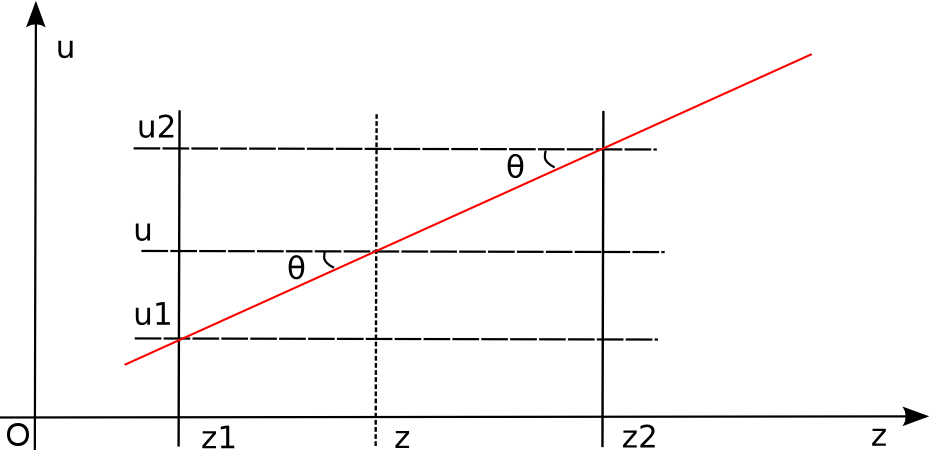
\includegraphics[width=12cm]{./figures/schema_resolution_tel.png}
%       \caption{Schema d'un telescope compos\'e de deux plans.}
%       \label{schema_reso}
%   \end{figure}

   \medskip

  Supposons une impulsion infinie et donc une trace rectiligne. La propagation de l'erreur selon $u$ en fonction de $u_1$et $u_2$ est donn\'ee par la relation suivante :
  
  \begin{equation}
   \Delta u ^2(u_1,u_2) = \left( \cfrac{\partial u}{\partial u_1} \right)^2 \Delta u_1 ^2 + \left( \cfrac{\partial u}{\partial u_2} \right)^2 \Delta u_2 ^2
  \end{equation}
  
  Exprimons alors $u$ en fonction de $u_1$ et $u_2$ :
  
  \begin{equation}
   \cfrac{u_2-u_1}{z_2-z_1} = \cfrac{u-u_1}{z-z_1} = \cfrac{u_2-u}{z_2-z}
  \end{equation}
  
  Donc : 
  
  \begin{equation}
   u (z_2 - z_1) = u_2 (z - z_2) + u_1 (z_2 -z)
  \end{equation}
  
  \begin{equation}
   u = \cfrac{z - z_1}{z_2 - z_1} u_2 + \cfrac{z_2 - z}{z_2 - z_1} u_1
  \end{equation}

   On obtient alors la relation de propagation de l'erreur suivante :

  \begin{equation}
   \Delta u ^2(z) = \left( \cfrac{z_2 - z}{z_2 - z_1} \right)^2 \Delta u_1 ^2 + \left( \cfrac{z - z_1}{z_2 - z_1} \right)^2 \Delta u_2 ^2
%   \label{eq:propag_erreurs}
  \end{equation}
  
  Les erreurs $\Delta u_1$ et $\Delta u_2$ correspondent alors aux r\'esolutions spatiales des plans 1 et 2. On peux alors \'ecrire : $\Delta u_1 = \sigma_1$ et $\Delta u_2 = \sigma_2$. Pour des pixels carr\'es, la relation est la m\^eme pour la r\'esolution spatiale selon l'axe $v$. Au final on obtient pour la r\'esolution du t\'elescope $\sigma_{tel}$ : 
  
  \begin{equation}
   \sigma_{tel}(z) = \sqrt{ \left( \cfrac{z_2 - z}{z_2 - z_1} \right)^2 \sigma_{1}^2 + \left( \cfrac{z - z_1}{z_2 - z_1} \right)^2  \sigma_{2}^2 }
  \label{eq:propag_erreurs}
  \end{equation}  
  
  Avec $\sigma_{1}$ la r\'esolution spatiale du plan 1 et $\sigma_{2}$ la r\'esolution spatiale du plan 2. Lorsque le point $z$ se situe au milieu des plans 1 et 2, la r\'esolution spatiale du t\'elescope vaut :
  
  \begin{equation}
   \sigma_{tel}\left(z=\cfrac{z_1+z_2}{2} \right) = \cfrac{\sqrt{\sigma_1^2 + \sigma_2^2}}{2} 
   \label{eq:milieuTel}
  \end{equation}
  
  Et en particulier lorsque $\sigma_1 = \sigma_2 = \sigma$ :
  
  \begin{equation}
    \sigma_{tel}\left(z=\cfrac{z_1+z_2}{2} ; \sigma_1 = \sigma_2 = \sigma \right) = \cfrac{\sigma}{\sqrt{2}}
    \label{eq:reso_milieu}
  \end{equation}

  Nous allons alors tracer la r\'esolution spatiale d'un t\'elescope compos\'e de deux plans en fonction de la position $z$ entre ces deux plans. Les positions $z_1$ et $z_2$ des deux plans sont fix\'ees \`a $z_1 = 0 \, cm$ et \`a $z_2 = 4 \, cm$. Diff\'erentes courbes r\'ealis\'ees \`a partir de diff\'erentes r\'esolutions spatiales pour les plans un et deux on \'et\'e trac\'ees. Nommons $\sigma_1$ la r\'esolution spatiale du premier plan et $\sigma_2$ celle du second plan. Les r\'esolutions utilis\'ees sont les suivantes : 

  \begin{figure}[!htb]
    \begin{center}
      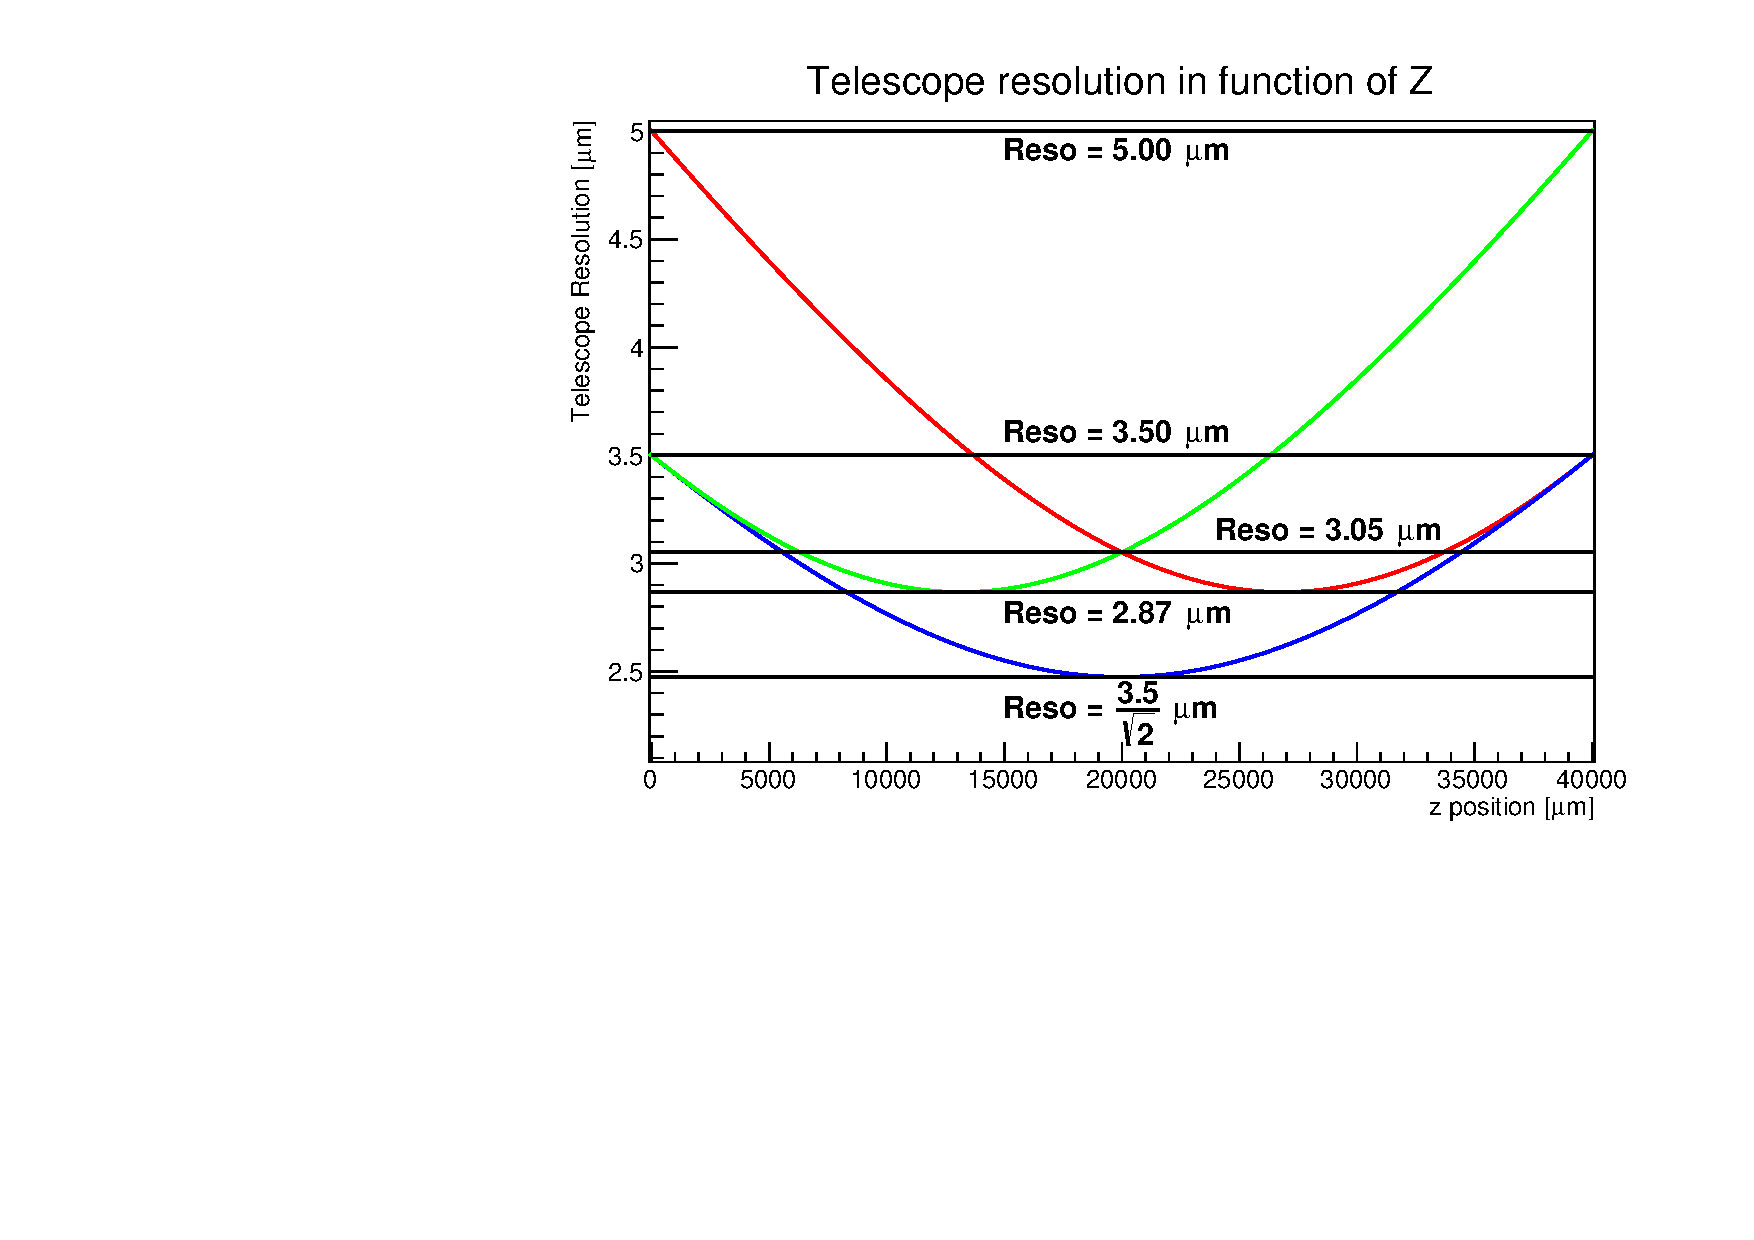
\includegraphics[scale=0.6]{./figures/Plot_reso_vs_z/reso_vs_Z2.pdf}
      \caption{R\'esolution d'un t\'elescope \`a deux plans en fonction de la position z entre ces deux plans. Les positions $z_1$ et $z_2$ des deux plans sont fix\'ees \`a $0 \, cm$ et $4 \, cm$. La courbe bleue repr\'esente la r\'esolution du t\'elescope obtenue avec une r\'esolution pour les deux plans de $3.5 \, \mu m$. La courbe rouge est r\'ealis\'ee \`a partir une r\'esolution de $5 \, \mu m$ pour le premier plan et de $3.5 \,\mu m$ pour le second plan. Enfin, la courbe verte r\'esulte d'une r\'esolution de $3.5 \, \mu m$ sur le premier plan et de $5.0 \, \mu m$ sur le second. Les maxima et minima sont indiqu\'es par des lignes horizontales. }
      \label{fig:resoTelescope_Z}
    \end{center}
  \end{figure}  
  
  \medskip
   
  \renewcommand{\labelitemi}{$\bullet$}
  
  \begin{itemize}
   \item Courbe bleue : $\sigma_1 = \sigma_2 = 3.50 \, \mu m$
   \item Courbe rouge : $\sigma_1 = 5.00 \, \mu m, \qquad \sigma_2 = 3.50 \, \mu m$
   \item Courbe verte : $\sigma_1 = 3.50 \, \mu m, \qquad \sigma_2 = 5.00 \, \mu m$
  \end{itemize}  

  \medskip
 
  Pour la courbe bleue, r\'ealis\'ee avec les m\^emes r\'esolutions spatiales $\sigma = 3.5 \, \mu m$ sur chacun des deux plans, la r\'esolution spatiale maximum vaut $3.5 \, \mu m$. Cette r\'esolution spatiale maximum est obtenue aux deux extr\'emit\'es $z_1$ et $z_2$ du t\'elescope. Le minimum est quant \`a lui observ\'e au milieu du t\'elescope en $z=2 \, cm$ et vaut comme nous l'avons vu avec l'\'equation \ref{eq:reso_milieu} $3.5/\sqrt{2} \, \mu m$. Dans cas, la r\'esolution spatiale du t\'elescope diminue entre $z=z_1$ et $z=(z_1+z_2)/2$, et remonte entre $z=(z_1+z_2)/2$ et $z=z_2$.
  
  \medskip
  
  Pour les courbes rouge et verte, la r\'esolution spatiale du t\'elescope en $z=z_1$ est \'egale \`a la r\'esolution spatiale du plan 1 puis cette r\'esolution diminue progressivement jusqu'au minimum. Ce minimum est obtenue quand la d\'eriv\'ee de l'expression \ref{eq:propag_erreurs} s'annule. Cette derni\`ere s'annule lorsque :
  
  \begin{equation}
   z = \cfrac{\sigma_2^2}{\sigma_1^2+\sigma_2^2} \, z_1 +  \cfrac{\sigma_1^2}{\sigma_1^2+\sigma_2^2} \, z_2
  \end{equation}

  Il suffit alors d'injecter cette valeur dans la relation \ref{eq:propag_erreurs} pour obtenir la valeur de la r\'esolution spatiale minimum du t\'elescope. Dans le cas, des courbes rouge et verte on obtient $\sigma_{Min} \approx 2.87 \, \mu m$. Cependant, ces valeurs de r\'esolutions spatiales minimales ne partagent pas le m\^eme $z$. Pour la courbe verte le minimum est atteint en $z=1.315 \, cm$ alors que pour la courbe rouge il est atteint en $z=2.685 \, cm$. Ensuite, \`a partir du minimum et jusqu'au plan 2, la r\'esolution spatiale du t\'elescope augmente pour atteindre la r\'esolution du plan 2 au niveau de ce dernier. On notera que ces deux courbes sont sym\'etriques par rapport au milieu du t\'elescope. De plus, les deux courbes se croisent au milieu du t\'elescope donnant lieu \`a une r\'esolution spatiale, calcul\'ee gr\^ace \`a l'\'equation \ref{eq:milieuTel}, valant $\sigma(z=(z_1+z_2)/2) \approx 3.05 \, \mu m$. 
 
  \medskip
  
  Supposons \`a pr\'esent un t\'elescope compos\'e de 4 plans de r\'esolution spatiale identique $\sigma_{ref}$ plac\'es aux positions respectives, $z_1$, $z_2$, $z_3$ et $z_4$. La r\'esolution du t\'elescope \`a la position $z$ est donn\'e par : 
  
  \begin{equation}
   \sigma_{tel}(z) = \dfrac{\sigma_{ref} }{ \sqrt{2} \left| \dfrac{z_1+z_2}{2} - \dfrac{z_3+z_4}{2} \right| } \sqrt{ \left( z-\dfrac{z_1+z_2}{2} \right)^2 + \left( \dfrac{z_3+z_4}{2} -z \right)^2  }
  \label{reso_tel_4_plans}
  \end{equation}

  
  \subsubsection{Calcul de la résolution du DUT.}

  Lors de l'analyse des donn\'ees, la valeur accessible est la largeur de la distribution des r\'esidus. Celle-ci est reli\'ee \`a la r\'esolution du DUT : $\sigma_{DUT}$, \`a la r\'esolution du t\'elescope : $\sigma_{Tel}$ et \`a l'erreur d\^u \`a la diffusion multiple : $\sigma_{ms}$, par la somme quadratique suivante :
  
  \begin{equation}
   \sigma_{Res}^2 = \sigma_{Tel}^2 + \sigma_{DUT}^2 + \sigma_{ms}^2
   \label{eq:resolution}
  \end{equation}
  
  \paragraph{Diffusion multiple}
  
  Voyons plus en d\'etail le cas de $\sigma_{ms}$ dans une configuration simple. Pour cela nous allons consid\'erer 3 plans de capteurs CMOS et des traces issues de particules charg\'ees \`a incidence normale. Le plan 2 est le DUT et les plans 1 et 3 constituent le t\'elescope (voir figure \ref{fig:schema_diff_multiple}). L'impulsion des particules est prise \`a 120 $GeV/c$ comme lors des tests en faisceau. L'angle moyen de d\'eviation de la trace apr\`es le passage \`a travers la mati\`ere du plan 2 est donn\'e par :
  
  \begin{equation}
   \theta = \cfrac{13.6 \, \text{MeV}}{\beta \, c \, p} \, Z \, \sqrt{\cfrac{x}{X0}} \left( 1+0.038 \ln \left(\cfrac{x}{X0} \right) \right) 
  \end{equation}

  On remarque alors que pour une m\^eme \'epaisseur de mat\'eriau, l'angle moyen de d\'eviation est proportionnel \`a $1/p$.
  Avec pour nos particules ultra-relativistes an a : $\beta c p = pc = 120 \, GeV$, $Z=1$ la charge de la particule, $x = 50 \, \mu m$ l'\'epaisseur du capteur 2 selon l'axe $z$ et $X0 = 9.36 \, cm$ la longueur de radiation du silicium. Apr\`es calcul on trouve :
  
  \begin{equation}
   \theta = 1.87 \times 10^{-6} \, rad
  \end{equation}
  
  \begin{figure}[!htb]
    \begin{center}
      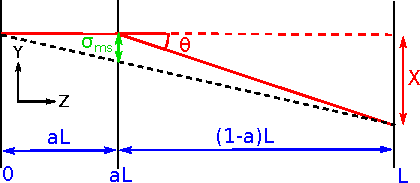
\includegraphics[scale=1.5]{./figures/diffusion_multiple.pdf}
      \caption{Sch\'ema de la diffusion multiple d'une trace passant \`a travers un capteur. La trace est d\'evi\'ee d'un angle $\theta$ et arrive sur un second capteur avec un d\'ecalage $X$. L'erreur due \`a la diffusion multiple est indiqu\'ee par $\sigma_{ms}$.}
      \label{fig:schema_diff_multiple}
    \end{center}
  \end{figure}  
  
  Voyons \`a pr\'esent comment on peut obtenir la valeur de $\sigma_{ms}$. La figure \ref{fig:schema_diff_multiple} d\'efinit $\sigma_{ms}$ en fonction de l'angle de d\'eviation $\theta$ et de la position du plan 2 sur lequel on veut mesurer $\sigma_{ms}$. Sur cette figure, une trace \`a incidence normale arrive \`a partir du plan 1 sur le plan 2. La trace est ensuite d\'evi\'ee d'un angle $\theta$ par le plan 2 et arrive avec un d\'ecalage $X$ selon l'axe $Y$ sur le troisi\`eme capteur. On veut alors connaître l'influence de la diffusion multiple sur le second capteur (c'est-à-dire le \textit{DUT}). $\sigma_{ms}$ est d\'efinie par l'erreur induite sur le plan 2 lorsque l'on reconstruit la trace \`a partir des plans 1 et 3. 
  
  \medskip
  
  A partir de cette figure, on a :
  
  \begin{equation}
   \cfrac{\sigma_{ms}}{aL} = \cfrac{X}{L}
   \label{eq:ms1}
  \end{equation}
   
   et :
   
  \begin{equation}
   \tan(\theta) = \cfrac{X}{(1-a)L}
   \label{eq:ms2}
  \end{equation}

  Lorsque l'on remplace le $X$ pris dans l'\'equation \ref{eq:ms1} avec celui de l'\'equation \ref{eq:ms2} on obtient la relation suivante :
  
  \begin{equation}
   \sigma_{ms} = a \, L \, (1-a) \, \tan(\theta)
  \end{equation}

  \begin{figure}[!htb]
    \begin{center}
      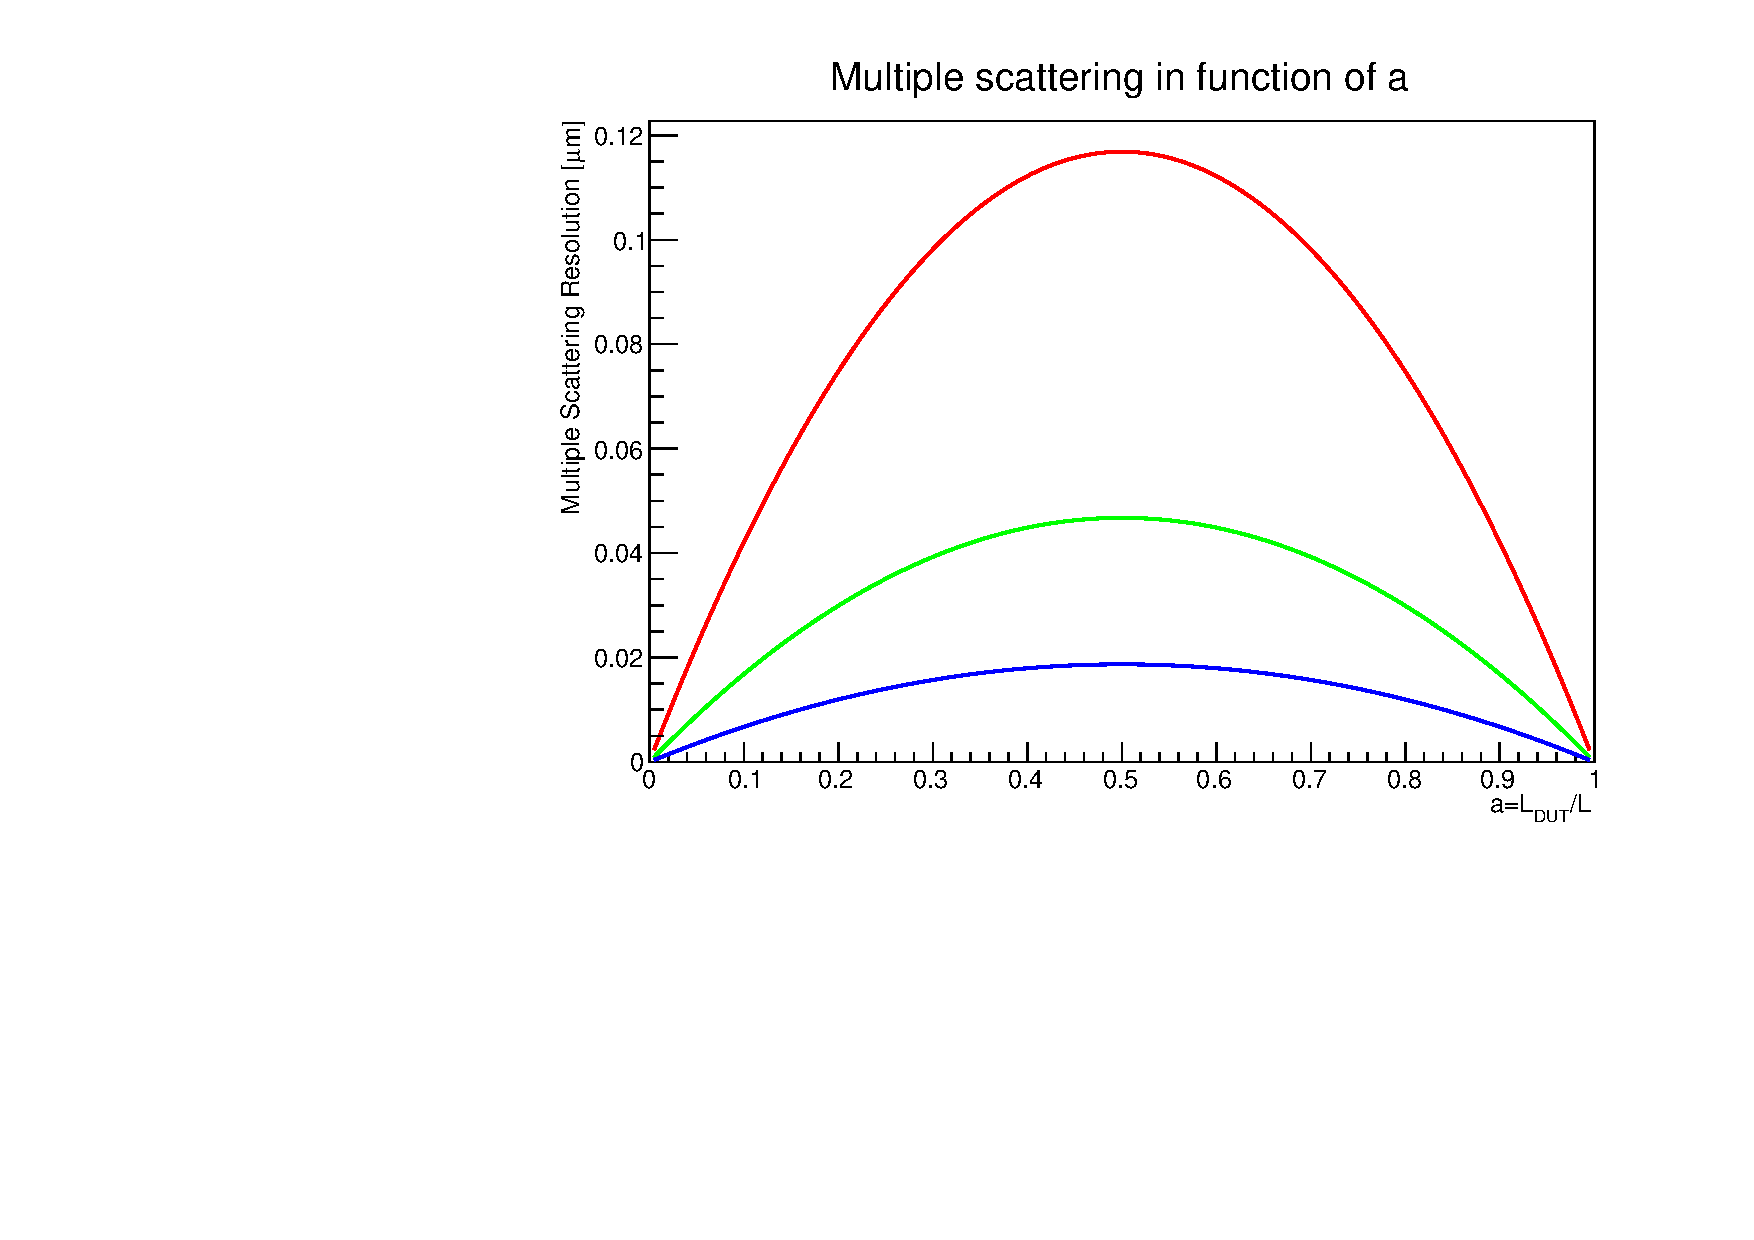
\includegraphics[scale=0.6]{./figures/Plot_reso_vs_z/multiple_scattering_4cm_pl1-pl3.pdf}
      \caption{$\sigma_{ms}$ en fonction de la position du DUT entre les plans 1 et 3. La courbe rouge correspond \`a une distance $L$ entre les plans 1 et 3 de $L = 25 \, cm$. Les courbes verte et bleue correspondent \`a respectivement $L = 10 \, cm$ et $L = 4 \, cm$. }
      \label{fig:diff_multiple_plot}
    \end{center}
  \end{figure}
  
  Nous allons \`a pr\'esent tracer $\sigma_{ms}$ en fonction du rapport de distance $a=L_{DUT}/L$. Pour cela nous allons prenons des distances valant $L = 4 \, cm$, $L = 10 \, cm$ et $L = 25 \, cm$ entre les plans 1 et 3. Les r\'esultats sont visibles en figure \ref{fig:diff_multiple_plot}. On remarque que $\sigma_{ms}$ devient de plus en plus grand lorsque la distance $L$ augmente. Pour une distance $L$ fix\'ee, la largeur $\sigma_{ms}$ est nulle en $a=0$ et augmente progressivement jusqu'\`a son maximum obtenu pour $a=0.5$. Puis $\sigma_{ms}$ diminue jusqu'\`a de nouveau atteindre $0$ en $a=1$. Les valeurs maximales obtenues pour $\sigma_{ms}$ en $a=1/2$ pour $L = 4 \, cm$, $L = 10 \, cm$ et $L= 25 \, cm$ valent respectivement environ $1.87 \times 10^{-2} \, \mu m$, $4.68 \times 10^{-2} \, \mu m$ et $1.17 \times 10^{-1} \, \mu m$.
  
  \medskip
  
  Si l'on prend par exemple le cas avec $L=10 \, cm$ et $a=1/2$. On a $\sigma_{ms}^2 = 2.19 \times 10^{-3} \, \mu m^2$. La diffusion multiple est donc n\'egligeable dans ce cas. 
  
  \medskip
  
  Pour une m\^eme configuration, lorsque l'impulsion des particules diminue, $\theta$ augmente en $1/p$. Cela implique donc une augmentation de la diffusion multiple. Dans notre configuration, la diffusion multiple n'est plus n\'egligeable pour des impulsions inf\'erieures \`a environ 5 $GeV/c$. Par exemple, \`a 5 $GeV/c$, dans la m\^eme configuration que pr\'ec\'edemment avec $L=10 \, cm$ et $a=1/2$, obtient $\theta = 4.49 \times 10^{-5}$ rad et $\sigma_{ms}^2 = 1.26 \, \mu m^2$.
  
  \medskip

  Ainsi, on constate dans notre cas simple \`a 3 trois plans de t\'elescope, lorsque la diffusion multiple est non n\'egligeable, qu'il faut rapprocher le DUT des plans l'entourant pour minimiser l'effet de la diffusion multiple.
  
%   De plus, nous avons vu qu'avec un t\'elescope compos\'e de deux plans de m\^eme r\'esolution spatiale, il faut centrer le DUT pour optimiser la largeur des r\'esidus. Cependant lorsque les r\'esolutions spatiales ne sont plus identiques il faut d\'ecaler le DUT pour minimiser la r\'esolution du t\'elescope. Dans le cas d'une forte diffusion multiple il faudra donc optimiser la position des plans de t\'elescope pour minimiser la largeur de la distribution des r\'esidus.
  
%   Si l'impulsion des particules traversant les capteurs est suffisamment grande,

\section{PLUME}

  \subsection{Motivations}

  Comme nous l'avons vu au chapitre pr\'ec\'edent, les \'echelles PLUME pourront être utilisées dans la boite AID. Un prototype d'\'echelle \textit{PLUME} a \'et\'e con\c{c}u en 2011. L'objet de cette section sera l'étude des performances et des caract\'eristiques de ce prototype d'\'echelle \textit{PLUME}. Les tests en faisceau d'une \'echelle \textit{PLUME} ont eu lieu en Novembre 2011 au SPS, au CERN \`a Gen\`eve. Les motivations principales de cette campagne de tests étaient :  
  
  \medskip
  
  \renewcommand{\labelitemi}{$\bullet$}
  
  \begin{itemize}
   \item la v\'erification du bon fonctionnement de l'\'echelle,
   \item l'étude de l'homog\'en\'eit\'e de la r\'eponse des capteurs,
   \item l'\'etude des mini-vecteurs,
   \item l'\'etude des d\'eformations de l'\'echelle.
  \end{itemize}

  \medskip

  Les \'etudes sur la d\'eformation de l'\'echelle ne seront pas abord\'ees en d\'etail dans cette th\`ese. Nous commencerons notre \'etude en d\'ecrivant la configuration exp\'erimentale. Puis nous commenterons les r\'esultats obtenus. Pour cela nous rappellerons les caract\'eristiques du capteur MIMOSA26 mont\'e 12 fois sur l'\'echelle, puis nous comparerons les r\'esultats obtenus pour chaque capteur de l'\'echelle. Enfin, nous finirons avec une \'etude sur les mini-vecteurs.
  
  \subsection{Configuration exp\'erimentale}
 % le setup exp\'erimental 
 
   Nous allons d\'ebuter par la description de la configuration exp\'erimentale utilis\'ee lors de cette campagne de tests en faisceau.
   
  \subsubsection{Faisceau du SPS}
  
  Les tests ont \'et\'e r\'ealis\'es dans le Hall Nord du SPS au CERN. La ligne utilis\'ee \'etait la ligne H6. Le fonctionnement est le suivant. Des protons dot\'es d'une impulsion de 400-450 $GeV/c$ sont extraits du SPS et interagissent avec la cible $T4$. \`A la sortie de cette cible un faisceau constitu\'e d'\'electrons, de hadrons et de muons d'impulsions comprises entre environ 5 et 205 $GeV/c$ est constitu\'e. Pour nos tests nous avons utilis\'e des pions charg\'es n\'egativement et dot\'es d'une impulsion de $120 GeV/c$. Les $\pi^-$ utilis\'e sont alors au dessus d'environ $30\%$ de leur minimum d'ionisation (voir section \ref{sect:bethe_bloch}). La structure temporelle du faisceau est la suivante. Le faisceau est d\'evers\'e durant 9.6 $s$ puis un temps mort de 37.2 secondes est observ\'e.
  
  \subsubsection{T\'elescope}

  Le t\'elescope utilis\'e est compos\'e de 4 plans r\'epartis en 2 bras de 2 plans chacun. Chaque plan est \'equipé de capteurs MIMOSA-26 amincis \`a 120 $\mu m$. Le DUT, c'est-à-dire l'\'echelle PLUME, est plac\'e entre les deux bras du télescope \`a l'exception des prises de donn\'ees \`a grand angle où le DUT est plac\'e \`a l'ext\'erieur du t\'elescope pour des raisons d'encombrement. On d\'efinit l'axe $Oz$ du t\'elescope comme l'axe parall\`ele au faisceau passant par le point $O(0,0,0)$ pris au centre de l'\'echelle PLUME selon son \'epaisseur et au milieu de l'\'echelle selon ses coordonn\'ees locales horizontale $U$ et verticale $V$. Le premier bras de télescope est plac\'e \`a $-85 \, mm$ selon l'axe $Oz$ par rapport au point $O(0,0,0)$ alors que le second bras est plac\'e \`a $+79 \, mm$ selon ce m\^eme axe. Les capteurs 1 et 2 appartenant au premier bras sont respectivement plac\'es \`a $-90 \, mm$ et $-80 \, mm$ selon l'axe $Oz$. Les capteurs 3 et 4 appartenant au second bras sont quant \`a eux plac\'es \`a $+74 \, mm$ et $+84 \, mm$ selon l'axe $Oz$.
  
    \begin{figure}[!htb]
    \begin{center} 
     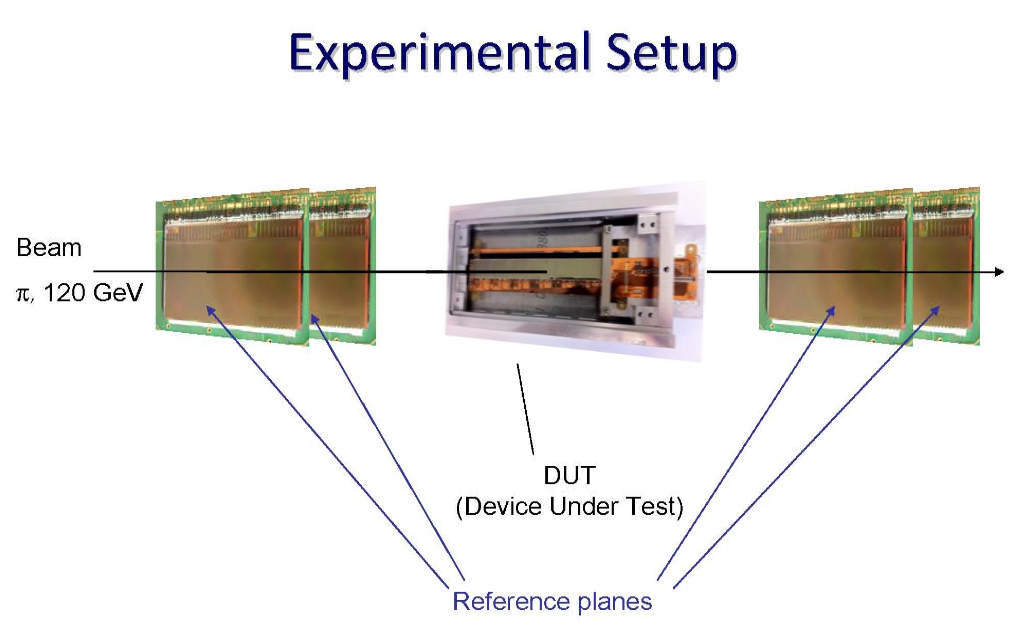
\includegraphics[scale=0.30]{./figures/Plots_PLUME/schema_montage.png}
     \caption{Schéma de la configuration de test.}
     \label{fig:confTelPLUME}
    \end{center}
  \end{figure}
  
  \begin{figure}[!htb]
    \begin{center} 
     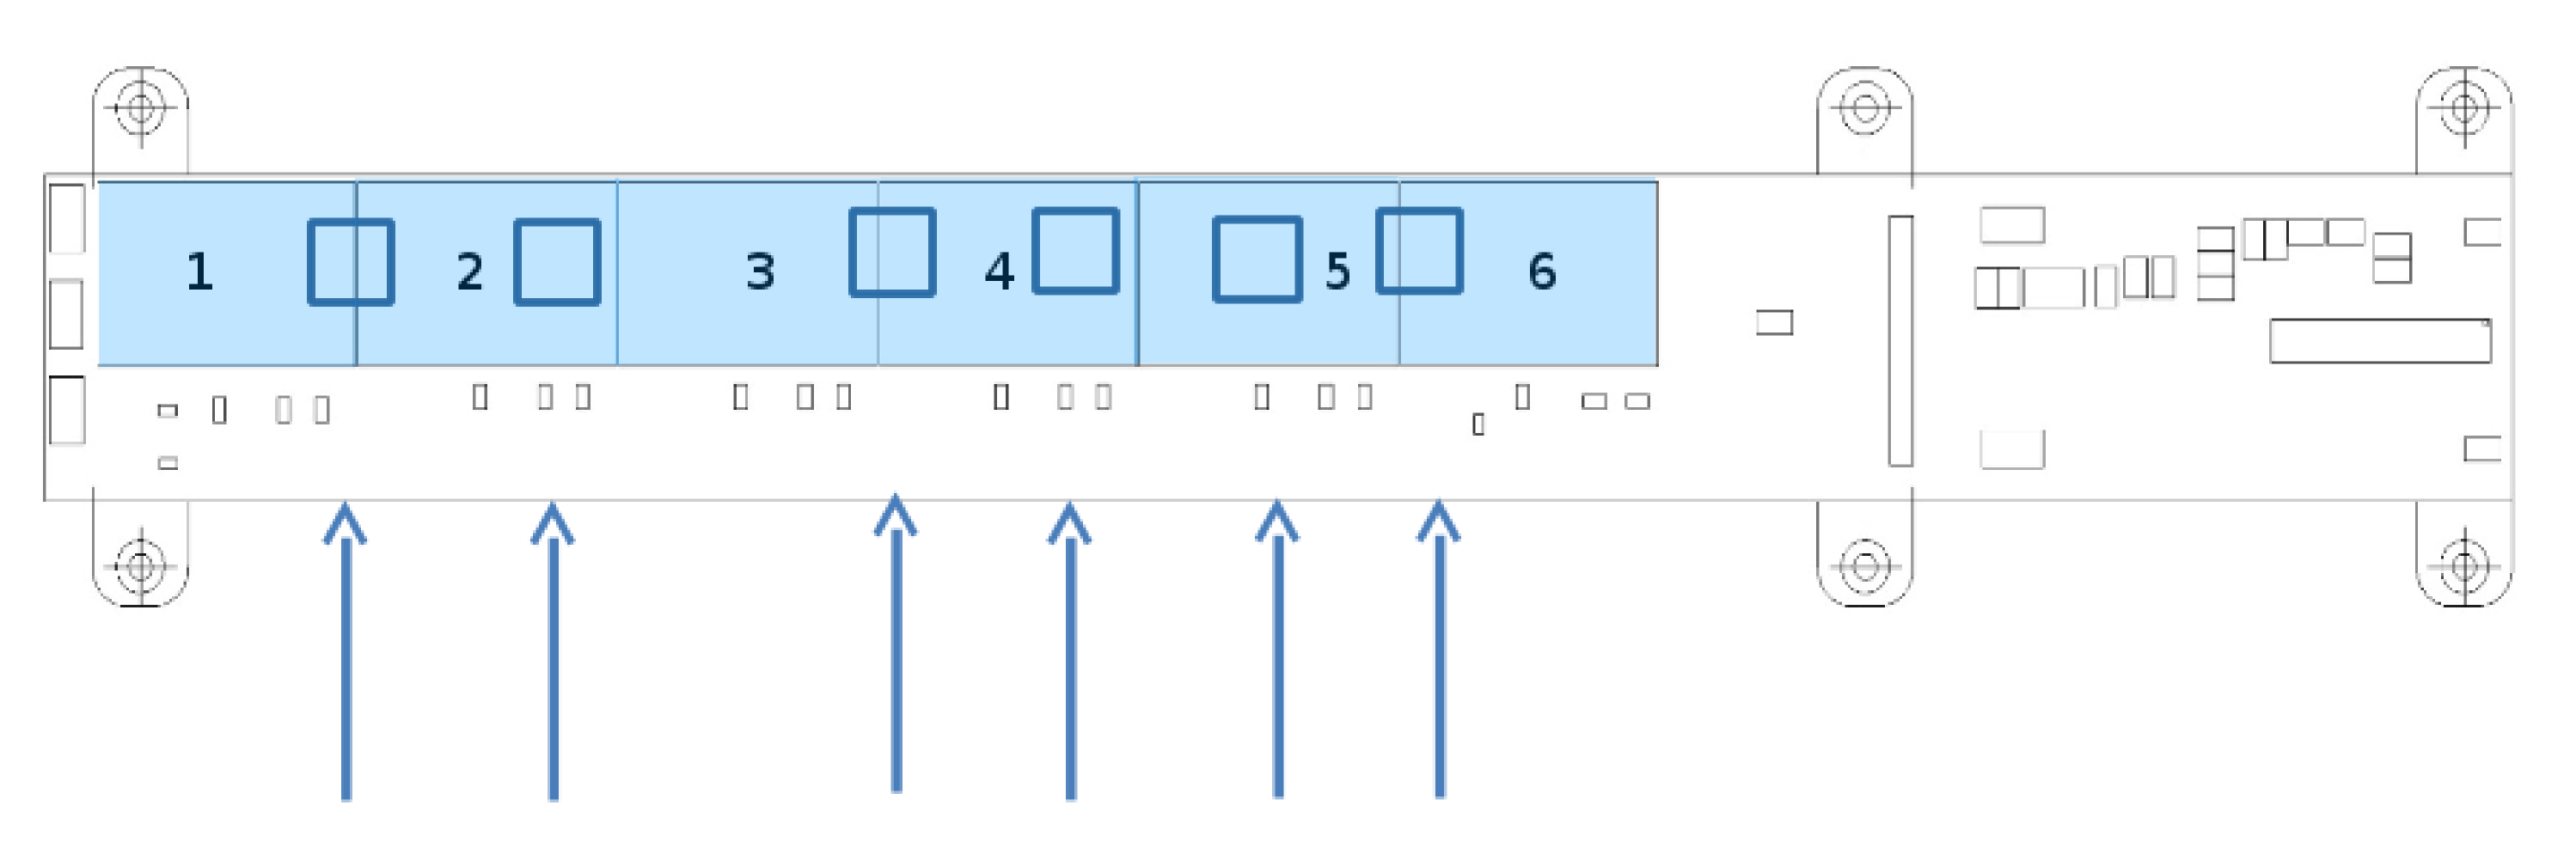
\includegraphics[scale=0.50]{./figures/Plots_PLUME/config_PLUME.png}
     \caption{Position des capteurs 1, 2, 3, 4, 5 et 6 sur l'\'echelle PLUME. Les capteurs sont indiqu\'es en bleu clair et sont nomm\'es de 1 \`a 6. Les carr\'es bleus fonc\'es repr\'esentent les positions du scintillateur (servant \`a d\'eclencher) lors des prises de donn\'ees. Les deux faces de l'\'echelle PLUME sont nomm\'es $OKF3$ et $OKF6$. $OKF3$ est la partie de l'\'echelle croisant le faisceau en premier alors que $OKF6$ repr\'esente la face oppos\'ee.}
     \label{fig:runsPLUME}
    \end{center}
  \end{figure}
  
  Dans le but de tester l'homog\'en\'eit\'e de la r\'eponse des capteurs, chaque zone de l'\'echelle PLUME a \'et\'e test\'ee. Une illustration d'une face de l'\'echelle PLUME est donn\'ee en figure \ref{fig:runsPLUME}. Les 6 capteurs de la face pr\'esent\'ee sont color\'es en bleu clair. 
  Ils sont num\'erot\'es de 1 \`a 6 pour chacune des faces. Dans la suite de ce chapitre on nommera la face travers\'ee par le faisceau en premier : $OKF3$ et la face oppos\'ee : $OKF6$. Pour la face \textit{OKF3} les positions des capteurs ainsi que les positions du faisceau sur l'\'echelle lors des différents tests sont illustr\'es en figure \ref{fig:runsPLUME}. En face du capteur 1 de la face \textit{OKF3} se trouve le capteur 1 de la face \textit{OKF6} et ainsi de suite jusqu'au capteur 6.
  
  \medskip
  
  Les positions du faisceau sur l'\'echelle lors des diff\'erentes prises de donn\'ees sont illustr\'ees par des carr\'es bleus fonc\'es sur la figure \ref{fig:runsPLUME}. Pour obtenir ces diff\'erentes positions, l'\'echelle PLUME \`a \'et\'e translat\'ee selon sont axe $U$. Un scintillateur de $7 \times 7 \, mm^2$ plac\'e \`a l'avant du t\'elescope a \'et\'e utilis\'e pour d\'eclencher. Pour chaque zone mise en faisceau, diff\'erents balayages selon le seuil des discriminateurs des capteurs de l'\'echelle PLUME ont \'et\'e r\'ealis\'es.

  \subsubsection{DAQ}

  Au niveau de l'acquisition, le nombre de capteurs lus simultan\'ement sur l'\'echelle \textit{PLUME} \'etait limit\'e \`a quatre capteurs. \'Etant donn\'e la taille du scintillateur de $7 \times 7 \, mm^2$, cela est suffisant puisque ce dernier peux couvrir au maximum une zone prise entre deux capteurs sur une face et donc de quatre capteurs sur les deux faces.
 
  \medskip
 
  Le taux de signaux de d\'eclenchement moyen au niveau du scintillateur \'etait de l'ordre de 1 \`a 8 $kHz$ au niveau du scintillateur. Cela correspond \`a un signal en moyenne toute les 100 $\mu s$ \`a $1 \, ms$. Cela autorise deux signaux de d\'eclenchements durant un temps de $112.5 \, \mu s$ correspondant \`a l'enregistrement d'une image du capteur. Cette image du capteur lu enti\`erement est appel\'e \textit{trame}. Dans certains cas le fort taux de signaux de d\'eclenchement am\`ene \`a r\'ealiser des \'ev\'enements comportant un nombre de trames plus important. Pour comprendre cela, nous allons donc \`a pr\'esent voir comment sont enregistr\'es les \'ev\'enements en fonction du signal de d\'eclenchement.
  
   \begin{figure}[!htb]
    \begin{center} 
     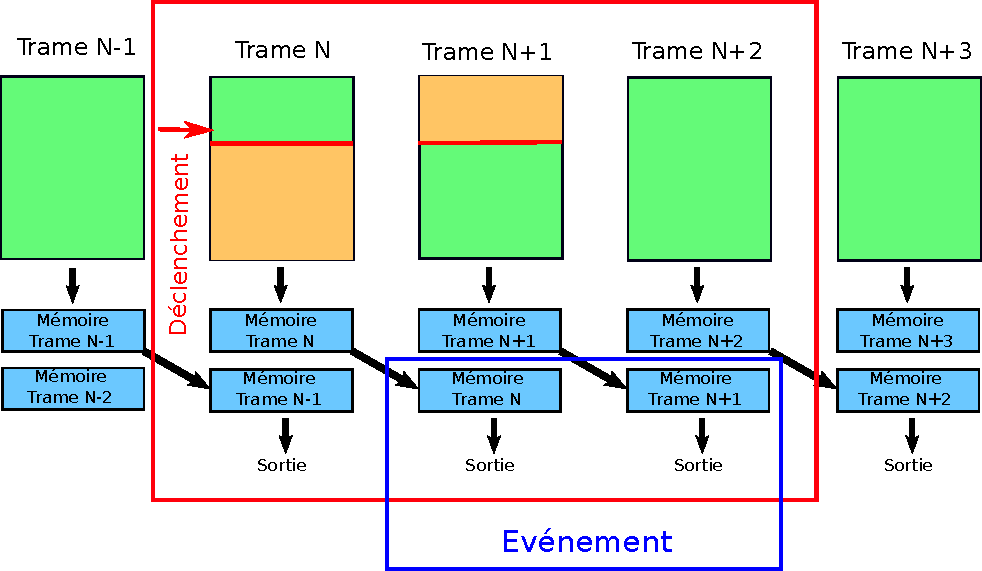
\includegraphics[scale=0.8]{./figures/lecture_Mi26_PLUME.pdf}
     \caption{Enregistrement des trames en fonction du signal de d\'eclenchement pour les capteurs de l'\'echelle \textit{PLUME} dans le cas g\'en\'eral. Chaque trame d'un capteur MIMOSA-26 est lue en $115.2 \, \mu s$.}
     \label{fig:1triggerFrames}
    \end{center}
   \end{figure}
  
  \medskip
  
  La figure \ref{fig:1triggerFrames} illustre la fa\c{c}on dont sont enregistr\'es les \'ev\'enements. Le signal de d\'eclenchement pr\'ec\`ede de quatre lignes la lecture de la ligne courante sur le capteur. Autrement dit pour obtenir la ligne correspondante au signal de d\'eclenchement, il faut ajouter la dur\'ee de lecture de quatre lignes au temps du d\'eclenchement. Comme le capteur comporte 576 lignes, si le signal de d\'eclenchement tombe entre la lecture de ligne 1 et la ligne 572 de la trame $N$, l'impact correspondant sur le capteur sera dans la trame $N$. Sinon, si le d\'eclenchement correspond \`a la lecture d'une ligne au-delà de la ligne 572, l'impact correspondant sera dans la trame $N+1$. Comme un \'ev\'enement doit correspondre \`a une trame compl\`ete, on lit les 576 lignes de l'\'ev\'enement reparties sur les trames $N$ et $N+1$. Sur la figure \ref{fig:1triggerFrames} un \'ev\'enement est indiqu\'e en orange. Par exemple, si le d\'eclenchement arrive \`a la ligne 96, on lira les lignes 100 \`a 576 de la trame $N$ puis les lignes 1 \`a 99 de la trames $N+1$. \`A la fin de sa lecture, chaque trame est enregistr\'ees dans une m\'emoire. Puis cette m\'emoire est transf\'erée vers une autre m\'emoire afin de stoker la trame suivante. Ainsi, lorsque l'on lit le capteur, lorsque la trame $N$ est en court de lecture, on r\'ecup\`ere les donn\'ees enregistr\'ee lors de la lecture de la trame $N-1$. Au final, on peut choisir soit de constituer un \'ev\'enement \`a partir de la ligne du d\'ebut de l'\'ev\'enement sur la trame $N$ jusqu'\`a la ligne de fin sur la trame $N+1$ ou de prendre les donn\'ees des deux trames $N$ et $N+1$. Dans notre cas un \'ev\'enement est construit \`a partir des deux trames compl\`etes $N$ et $N+1$.
  
  % 576-4 = 572

  \begin{figure}[!htb]
    \begin{center} 
     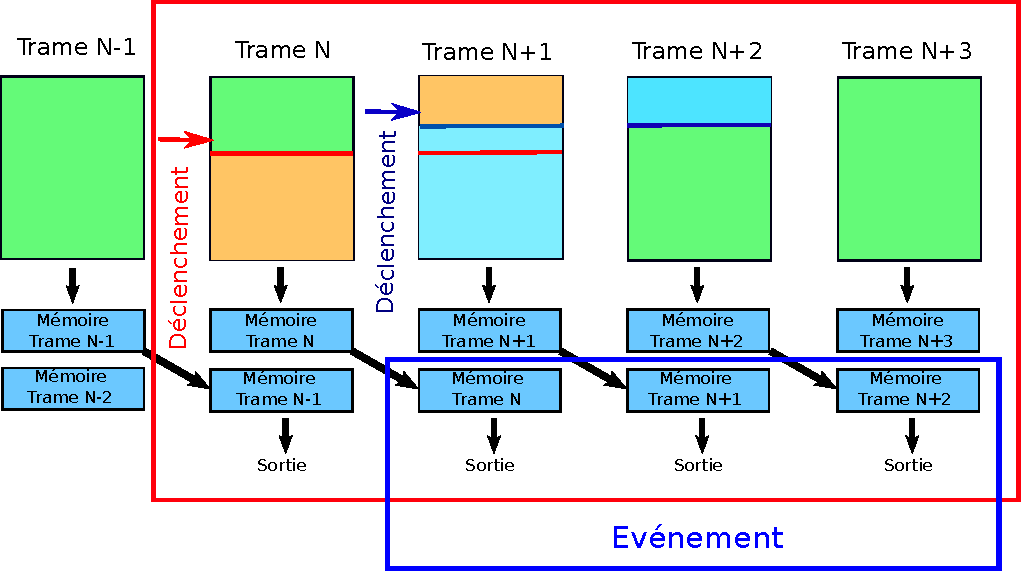
\includegraphics[scale=0.8]{./figures/lecture_Mi26_PLUME_2triggers.pdf}
     \caption{Enregistrement des trames en fonction du signal de d\'eclenchement pour les capteurs de l'\'echelle \textit{PLUME} dans le cas particulier discut\'e dans cette partie. Chaque trame d'un capteur MIMOSA-26 est lue en $115.2 \, \mu s$.}
     \label{fig:2triggerFrames}
    \end{center}
   \end{figure} 

   \medskip
 
   Comme nous l'avons vu deux signaux de d\'eclenchement peuvent parfois survenir durant la lecture des 576 lignes. Dans le cas ou un signal de d\'eclenchement suppl\'ementaire arrive au niveau de la trame $N+1$ avant la fin de l'\'ev\'enement (moins 4 lignes), on ajoute la trame $N+2$ \`a l'\'ev\'enement. La figure \ref{fig:2triggerFrames} illustre ce cas. Le premier \'ev\'enement est indiqu\'e en orange et est d\'elimit\'e par des lignes rouges. Un nouveau d\'eclenchement (fl\`eche bleue), arrive avant que 572 lignes soit lues. Dans ce cas une nouvelle trame est ajout\'ees \`a l'\'ev\'enement. L'extension de l'\'ev\'enement est indiqu\'e en bleu. Au final on peut choisir de constituer l'\'ev\'enement \`a partir de la premi\`ere ligne (premi\`ere ligne rouge) jusqu'\`a la derni\`ere ligne (derni\`ere ligne bleue fonc\'ee) ou de prendre les trois trames $N$, $N+1$ et $N+2$ compl\`ete. La derni\`ere option a \'et\'e choisie. On notera que si un nouveau d\'eclenchement arrive sur la trame $N+2$, 4 lignes avant la fin de l'\'ev\'enement (derni\`ere ligne bleue fonc\'ee), on r\'ep\`ete le processus et on ajoute une nouvelle trame. Ce processus est limit\'e \`a 100 trames maximum par \'ev\'enement.
 
%    Voyons \`a pr\'esent comment sont enregistr\'es les \'ev\'enements en fonction du signal de d\'eclenchement produit par le scintillateur \`a l'avant du télescope. Dans un cas simple o\`u un signal de d\'eclenchement arrive lors du d\'eroulement de l'enregistrement d'une trame \footnote{Trame : image obtenue apr\`es la lecture de tous les pixels d'un capteur. Une trame est appel\'ee \textit{frame} en anglais} cette trame et la suivante est enregistr\'ee. Lorsqu'un second signal de d\'eclenchement arrive lors de l'enregistrement de la seconde trame de l'\'ev\'enement, on ajoute une trame suppl\'ementaire \`a l`'\'ev\'enement. Une autre trame est encore ajout\'ee \`a l'\'ev\'enement si un signal de d\'eclenchement $n$ arrive sur la seconde trame après le dernier signal de d\'eclenchement $n-1$. Ce processus se r\'ep\`ete et une limite fix\'ee \`a 100 trames a \'et\'e utilis\'ee. 

%    On notera que le taux de signaux de d\'eclenchement moyen au niveau du scintillateur \'etait de l'ordre de 1 \`a 8 $kHz$ sur la surface du scintillateur. Ce qui correspond \`a un signal en moyenne toute les 100 $\mu s$ \`a $1 \, ms$. Cela autorise deux signaux de d\'eclenchements durant un temps de $112.5 \, \mu s$ correspondant \`a l'enregistrement d'une trame.

\subsection{R\'esultats : PLUME}

  Nous allons \`a pr\'esent exposer les r\'esultats obtenus en test en faisceau pour l'\'echelle PLUME. Pour cela, nous commencerons notre \'etude en rappelant les caract\'eristiques du capteur MIMOSA-26 mont\'e 12 fois sur l'\'echelle PLUME, puis nous comparerons les r\'esultats obtenus pour chaque capteur de l'\'echelle avec ceux du capteur de r\'ef\'erence. Nous regarderons alors si les r\'esultats obtenus pour chaque capteur sont homog\`enes. Enfin, nous finirons avec une \'etude sur les mini-vecteurs.
  
  \subsubsection{MIMOSA-26}
  
  \begin{figure}[!htb]
   \begin{center} 
    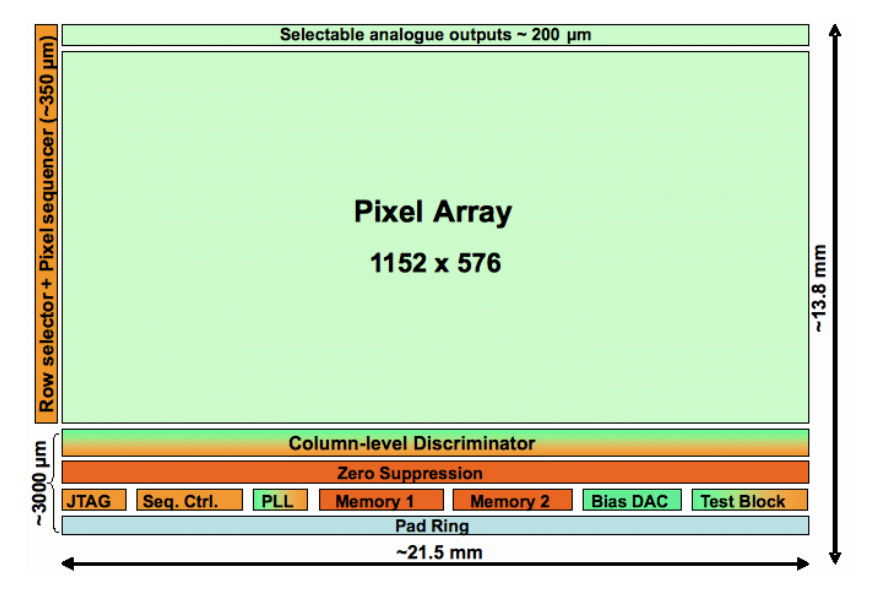
\includegraphics[scale=0.30]{./figures/schema_Mi26.png}
    \caption{Vue sch\'ematique de MIMOSA-26.}
    \label{fig:schema_Mi26}
   \end{center}
  \end{figure}
   
   MIMOSA-26 est le capteur final pour le télescope en faisceau \textit{EUDET} \cite{Perrey:2012gqa}. Son architecture est bas\'ee sur le capteur analogique MIMOSA-22 et sur le circuit de suppression de z\'eros \textit{SUZE-01}. Il est constitu\'e d'une matrice de $576 \times 1152$ pixels et est dot\'e d'un pas inter-pixel de 18.4 $\mu m$. Le capteur mesure $13.7 \times 21.5 \, mm^2$ et il poss\`ede une couche \'epitaxi\'ee, dite standard, \'epaisse de 14 $\mu m$. Il a \'et\'e r\'ealis\'e avec le proc\'ed\'e de gravure \textit{AMS} dot\'e d'une taille de grille de $0.35 \, \mu m$. MIMOSA-26 a \'et\'e con\c{c}u pour d\'etecter des particules charg\'ees avec un taux d'occupation de $10^6$ pixels$/cm^2/s$. Le capteur est lu gr\^ace au proc\'ed\'e de lecture en volet roulant en une dur\'ee de $115.2 \, \mu s$. Il poss\`ede une sortie fonctionnant \`a $80 \, MHz$. Chaque pixel contient un amplificateur et effectue un CDS. Chaque fin de colonne est \'equipée d'un discriminateur et une suppression de z\'ero est r\'ealis\'ee apr\`es num\'erisation du signal. On notera que le capteur est aussi \'equipé d'une sortie analogique beaucoup plus lente r\'eserv\'ee aux tests en laboratoire.   
    
  \begin{figure}[!htb]
   \begin{center} 
    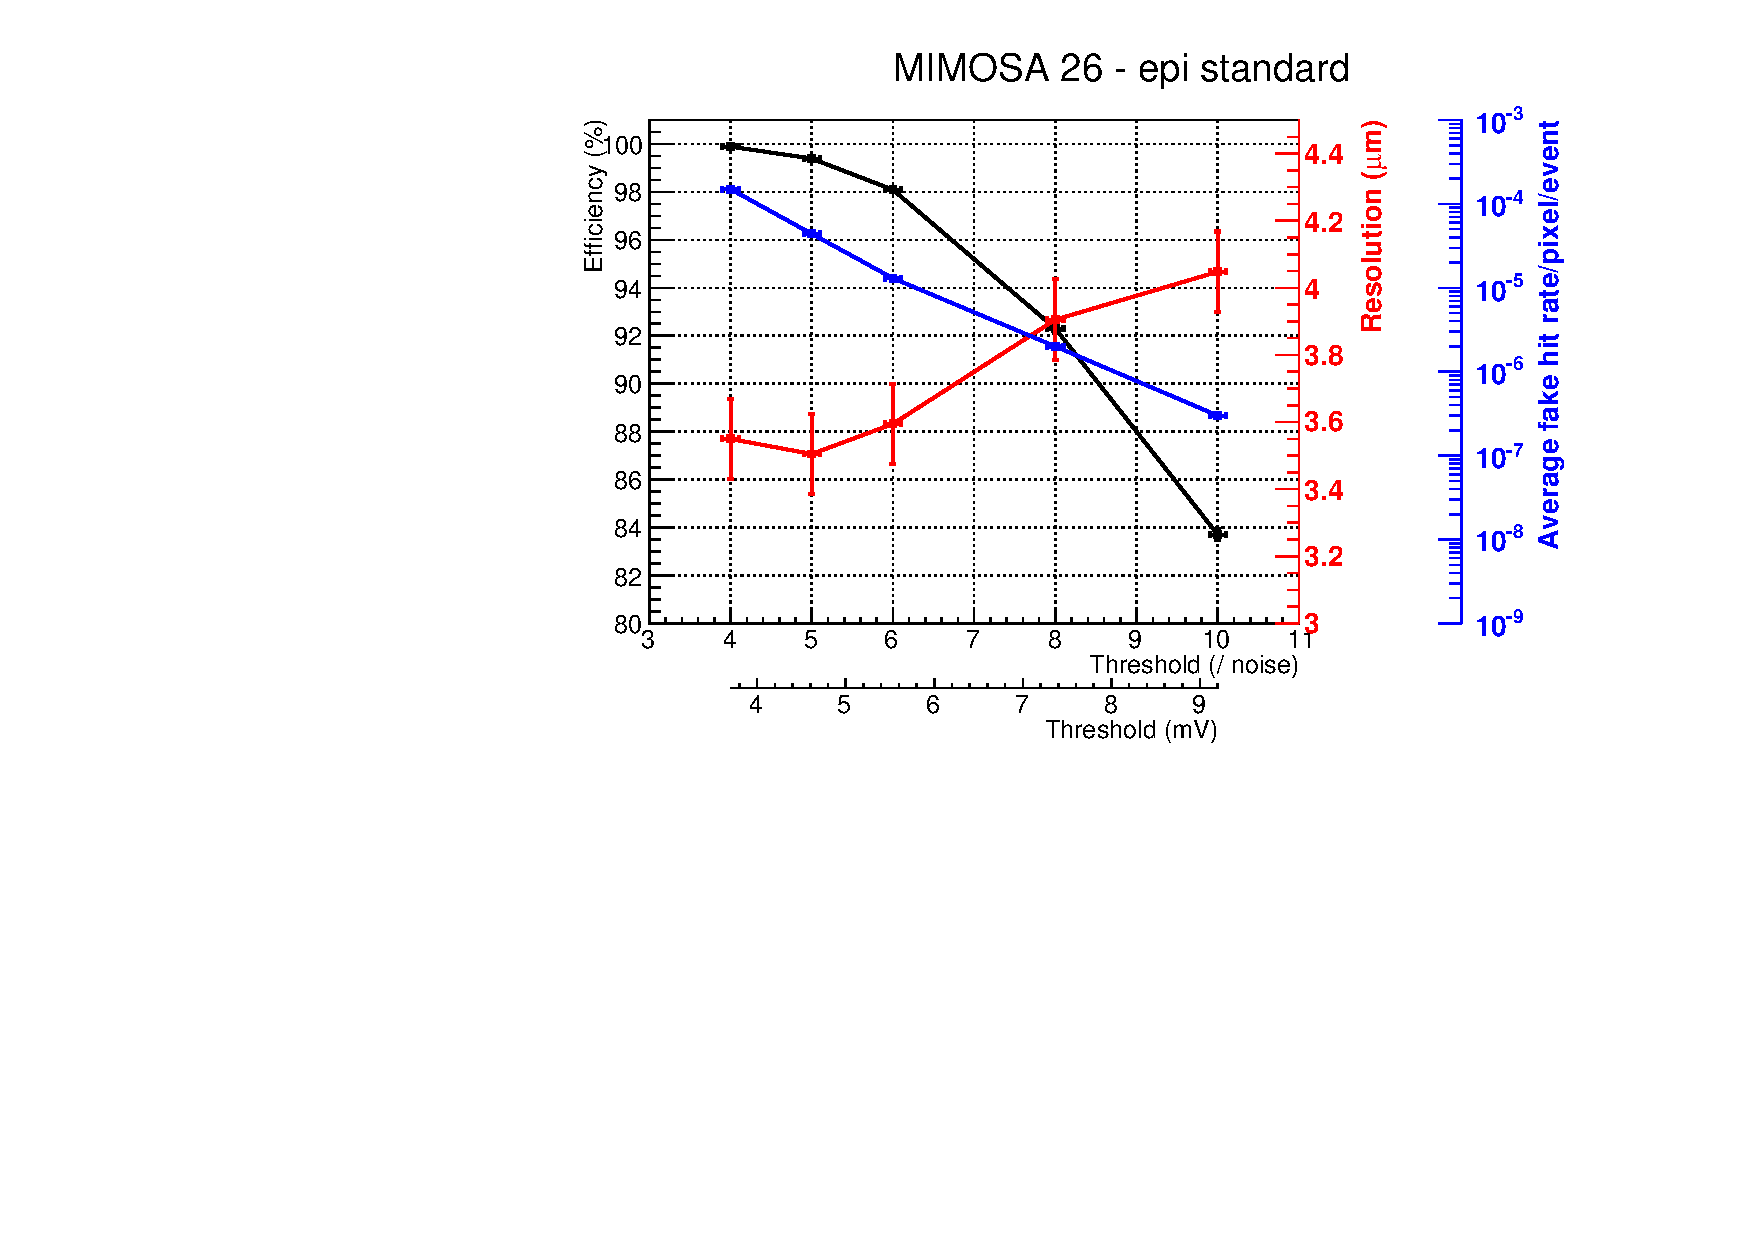
\includegraphics[scale=0.60]{./figures/Plots_PLUME/MIMOSA26_epi_std.pdf}
    \caption{Performances de MIMOSA-26. En noir l'efficacit\'e de d\'etection en fonction du seuil des discriminateurs, en bleu, le taux d'impacts fantômes en fonction du seuil, et en rouge, la r\'esolution spatiale en fonction du seuil.}
    \label{fig:perf_Mi26}
   \end{center}
  \end{figure}
   
   \medskip
   
   A son point de fonctionnement optimal, au seuil de 5 fois la largeur du bruit moyen, MIMOSA-26 pr\'esente une efficacit\'e d'environ 99.5 $\%$ pour un taux d'impacts fant\^omes inf\'erieurs \`a $10^{-4}$ et une r\'esolution spatiale d'environ $3.5 \, \mu m$. On notera que le taux d'impacts fant\^omes est domin\'e par un faible nombre de pixels plus bruyants ($\lesssim 1\%$) que les autres. La figure \ref{fig:perf_Mi26} illustre les performances de MIMOSA-26 en fonction du seuil des distriminateurs. Cette caract\'erisation a \'et\'e effectu\'ee au SPS \`a l'aide de pions charg\'es dot\'es d'une impulsion de l'ordre de 100 $GeV/c$. 
   
   \FloatBarrier
   
   \subsubsection{Alignement du t\'elescope}
   
   L'\'etape d'alignement du t\'elescope a \'et\'e la premi\`ere \'etape dans le processus d'analyse. Pour cet alignement nous avons utilis\'e une m\'ethode d'alignement utilisant quatre degr\'es de libert\'e : les trois positions du centre du capteur et une rotation du capteur selon l'axe $Oz$. Le capteur 1 a \'et\'e choisi comme r\'ef\'erence puis le capteur 4 a \'et\'e align\'e. Enfin les capteurs 2 et 3 on \'et\'e align\'es en fonction des capteurs 1 et 4. Les figures \ref{fig:resU_Pl2_Tel} et \ref{fig:resV_Pl2_Tel} montrent les distributions des r\'esidus prises sur le capteur 2 du télescope selon ses axes $U$ et $V$.
   
   \medskip
   
  \begin{figure}[!htb]
   \begin{center}
     \subfigure[R\'esidus sur l'axe horizontal $U$ du capteur 2 du t\'elescope.]{
      \label{fig:resU_Pl2_Tel}
      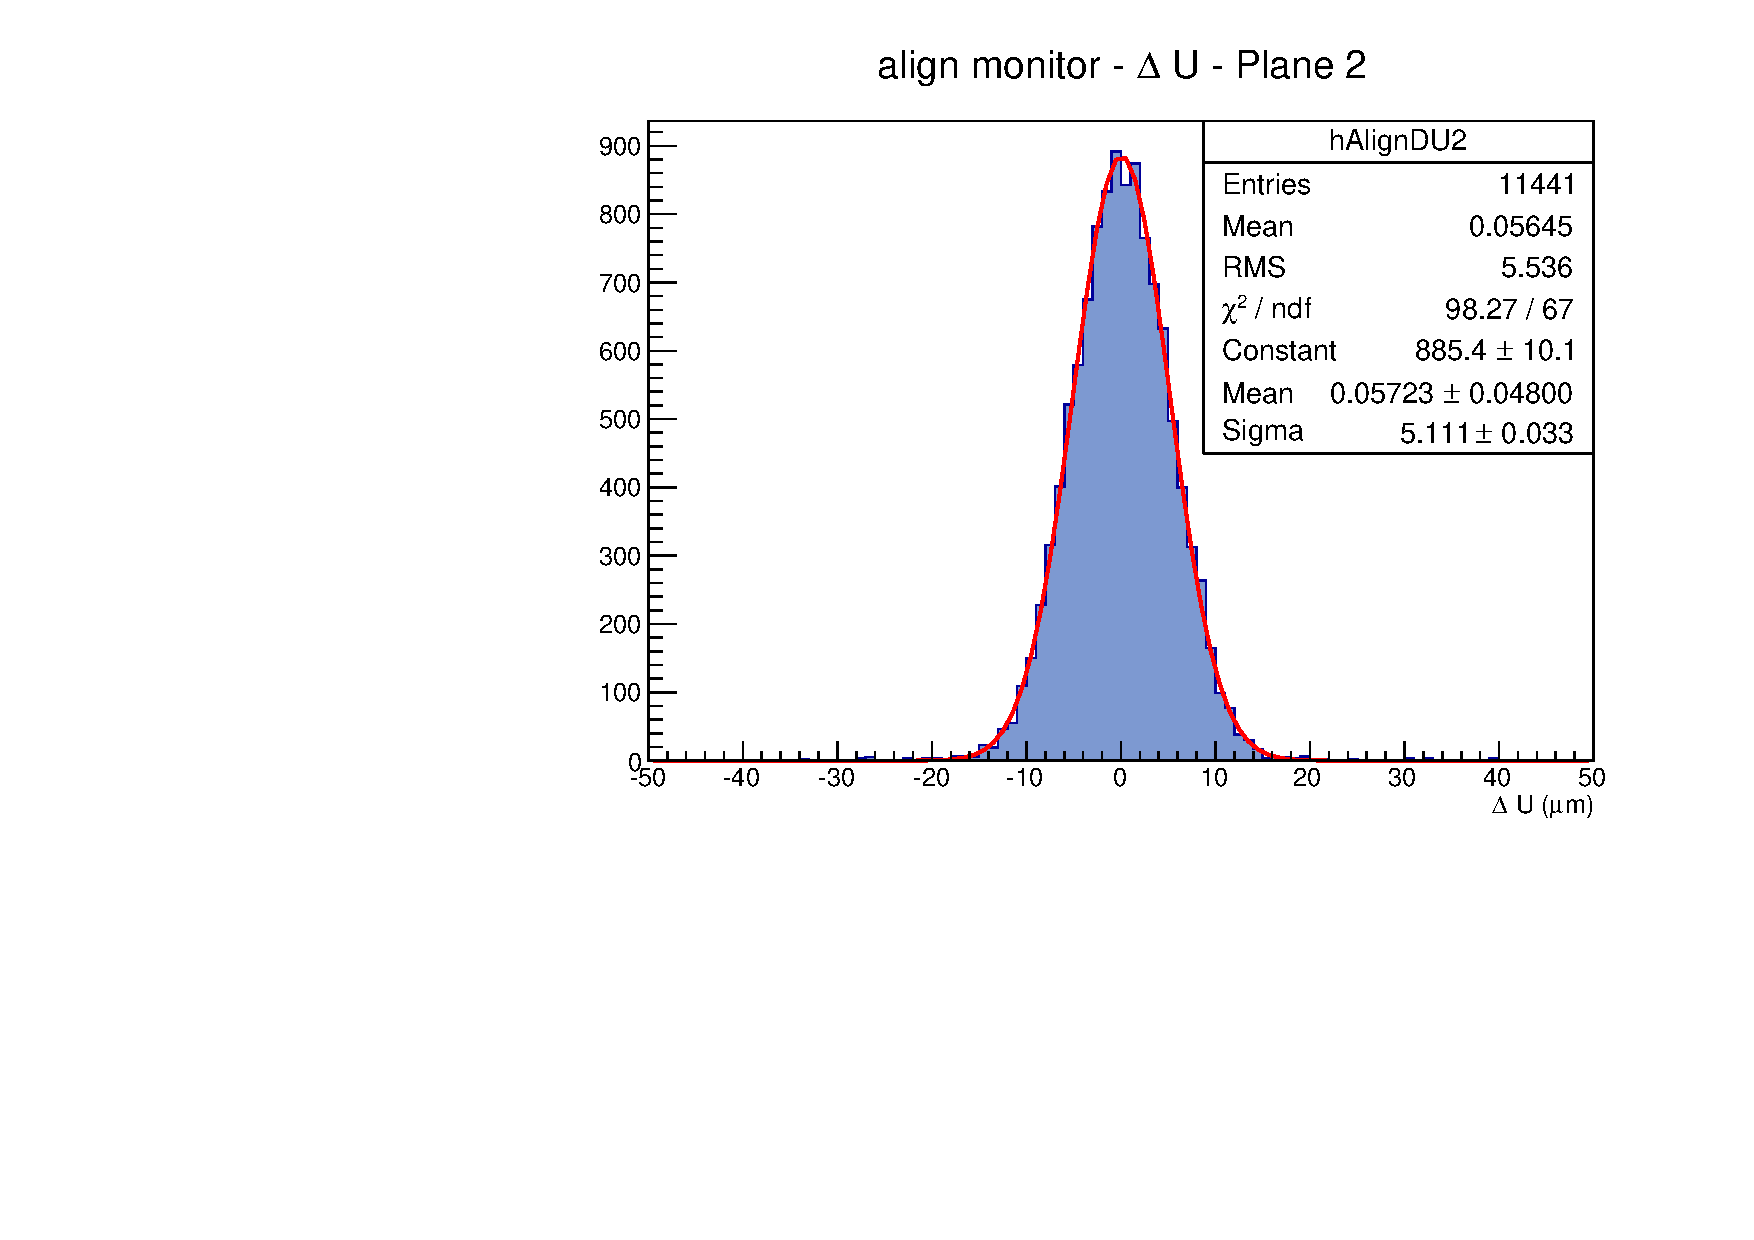
\includegraphics[width=0.47\textwidth]{./figures/Plots_PLUME/Alignement/Residus_U_Pl2_telescope.pdf}
     }
     \subfigure[R\'esidus sur l'axe vertical $V$ du capteur 2 du t\'elescope.]{
      \label{fig:resV_Pl2_Tel}
      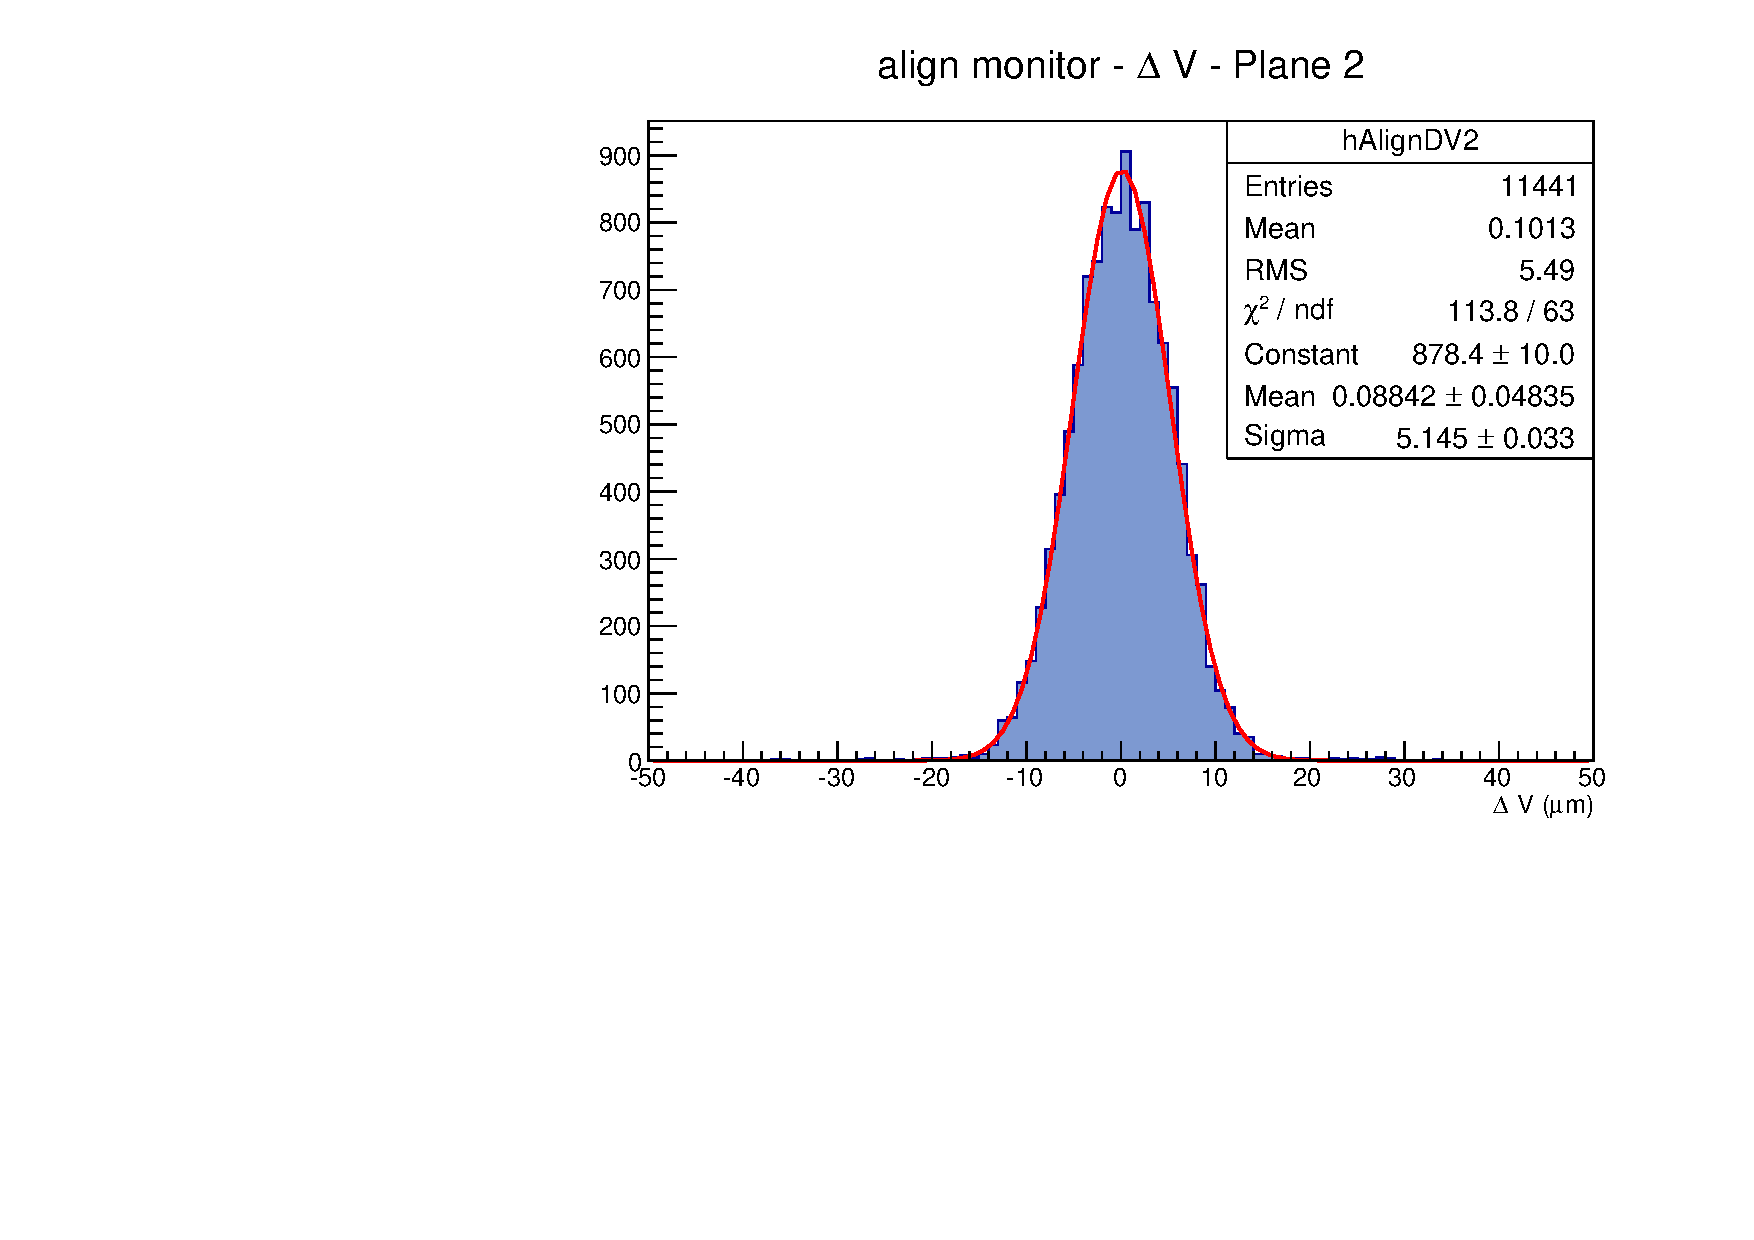
\includegraphics[width=0.47\textwidth]{./figures/Plots_PLUME/Alignement/Residus_V_Pl2_telescope.pdf}
     }
   \caption{R\'esidus sur le plan 2.}
   \label{fig:ReTelPLUME}
   \end{center}
  \end{figure}
   
%   \begin{figure}[!htb]
%    \begin{center} 
%     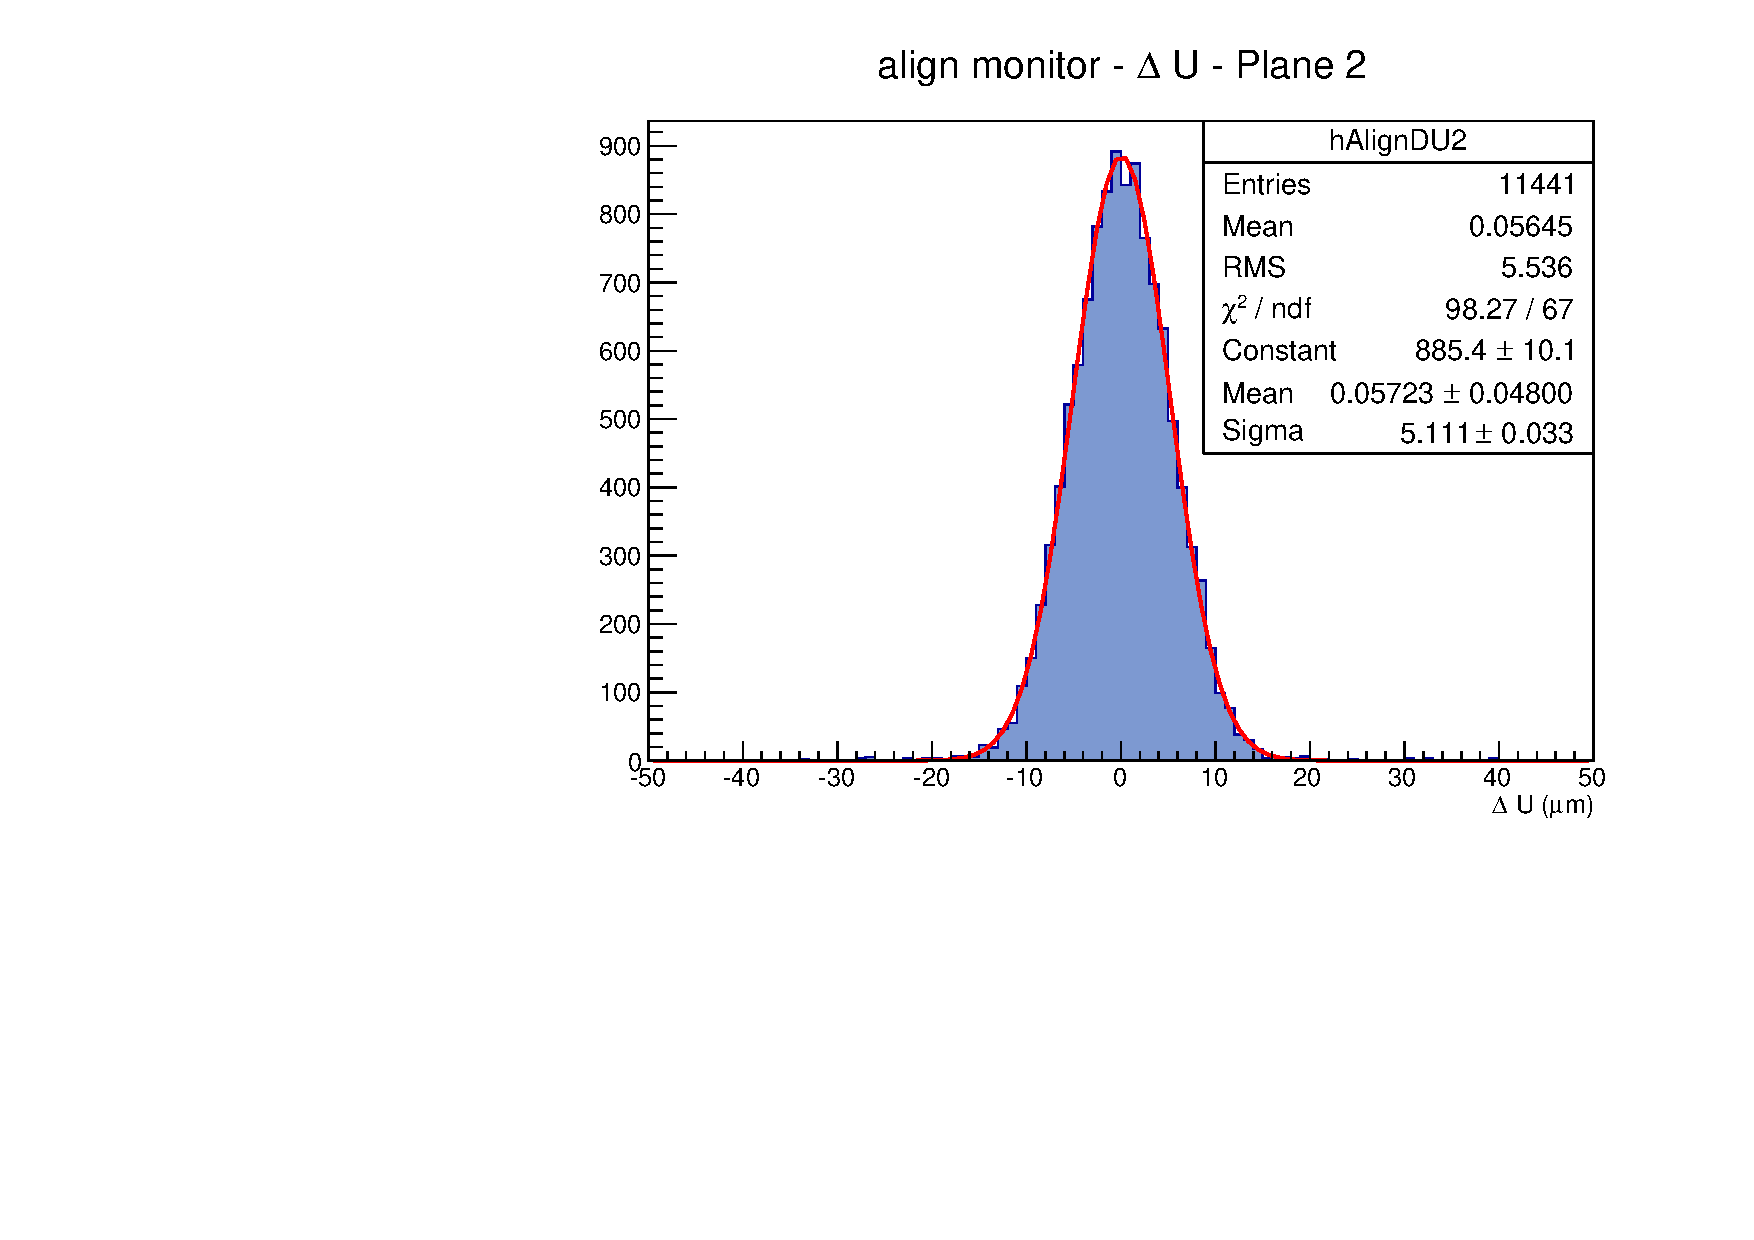
\includegraphics[scale=0.60]{./figures/Plots_PLUME/Alignement/Residus_U_Pl2_telescope.pdf}
%     \caption{R\'esidus sur l'axe horizontal $U$ du capteur 2 du t\'elescope.}
%     \label{fig:resU_Pl2_Tel}
%    \end{center}
%   \end{figure}
% 
%   \begin{figure}[!htb]
%    \begin{center} 
%     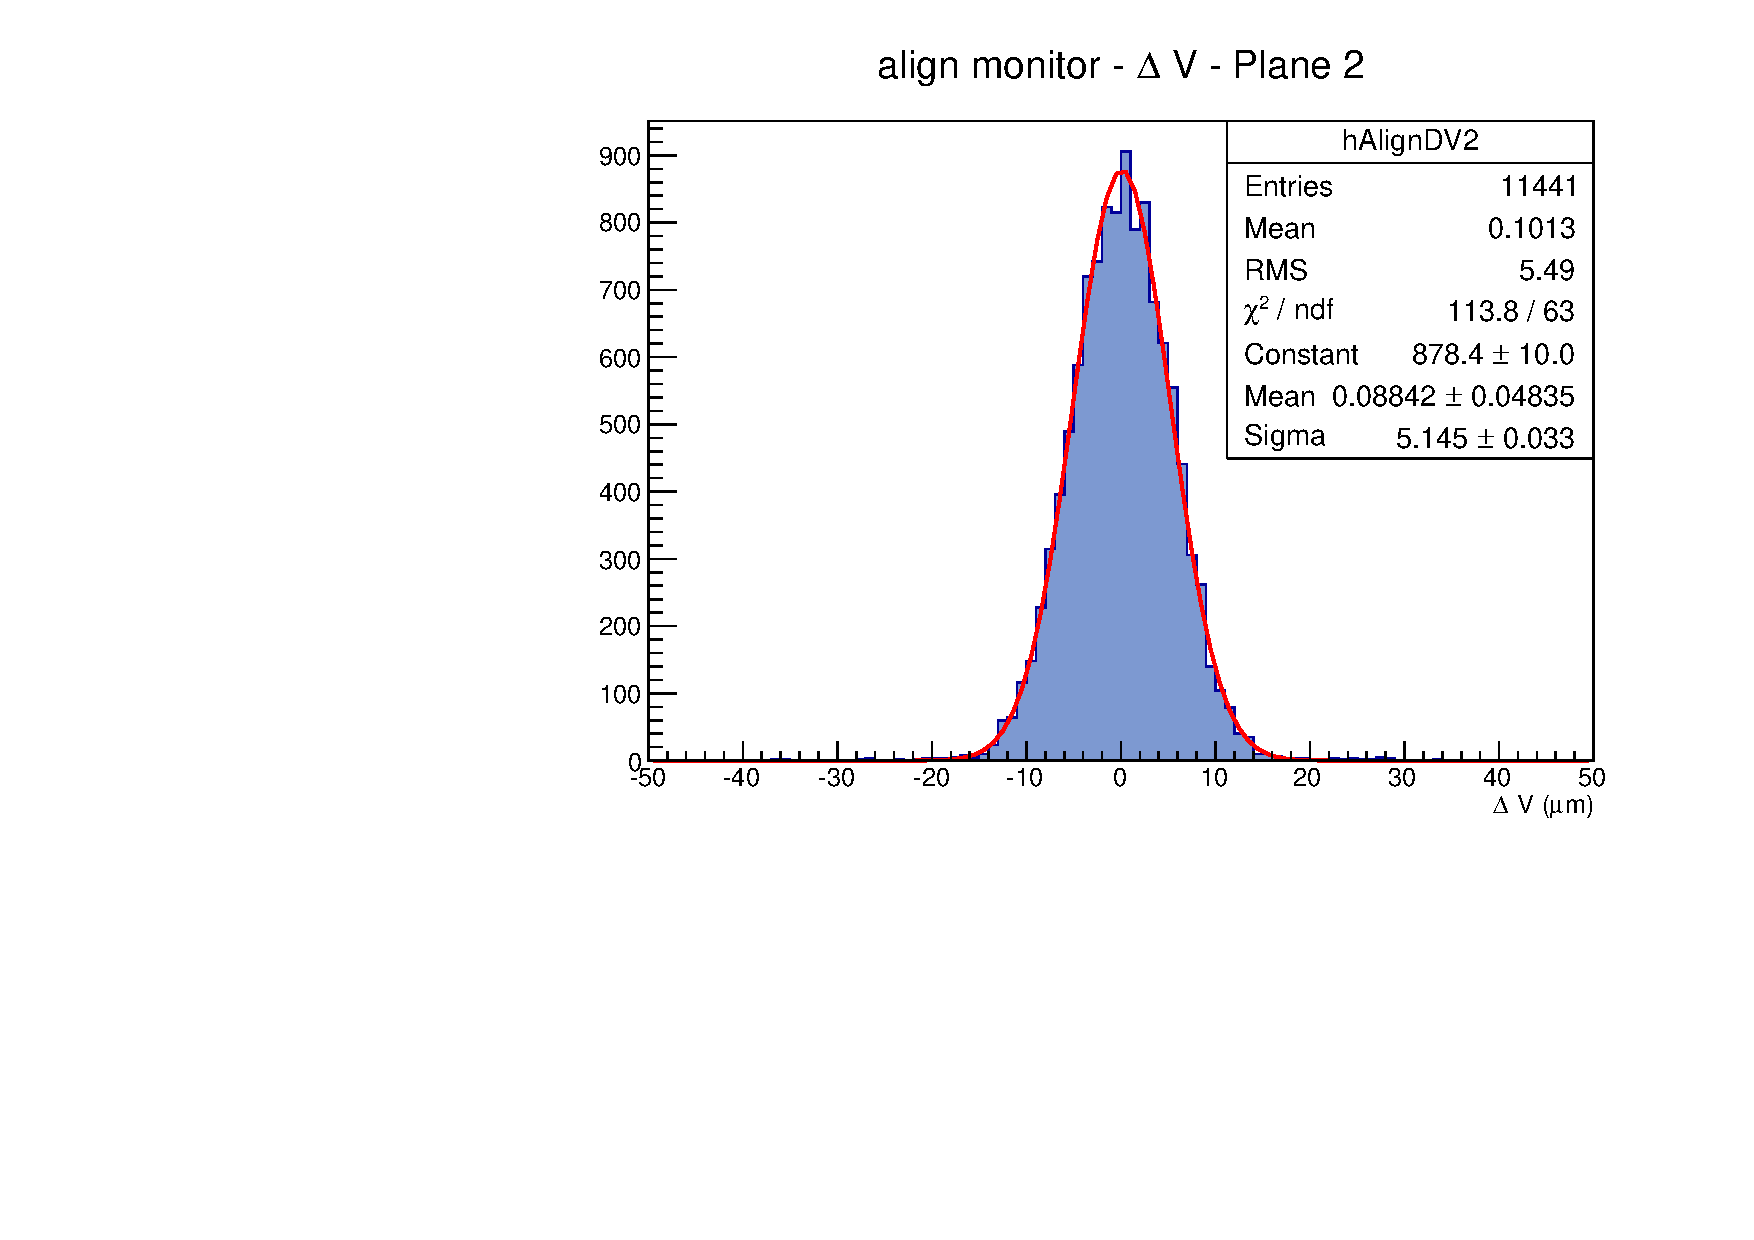
\includegraphics[scale=0.60]{./figures/Plots_PLUME/Alignement/Residus_V_Pl2_telescope.pdf}
%     \caption{R\'esidus sur l'axe vertical $V$ du capteur 2 du t\'elescope.}
%     \label{fig:resV_Pl2_Tel}
%    \end{center}
%   \end{figure}

  \medskip
  
  Les distributions des r\'esidus obtenues pour le capteur 2 du t\'elescope pr\'esente de l\'egers biais sur leur valeur moyenne. En effet, les valeurs moyennes de ces distributions ne sont pas centr\'ees en z\'ero. Le biais est inf\'erieur \`a 0.1 $\mu m$ pour le capteur 2 du t\'elescope mais peut atteindre jusqu'\`a 0.25 $\mu m$ pour le capteur 3. Ce biais est tr\`es certainement d\^u aux deux degr\'es de libert\'e non pris en compte dans la minimisation (rotation selon les axes U et V des capteurs). Comme le biais est faible, cela n'impacte que tr\`es peu la r\'esolution du télescope. Les r\'esultats pr\'esent\'es pour la partie \textit{PLUME} qui suivent sont obtenus avec cet alignement l\'eg\`erment biais\'e. Un alignement avec la nouvelle m\'ethode d'alignement \`a six degr\'es de libert\'es ajout\'ee au cours de cette th\`ese permet un meilleur alignement et permet de s'affranchir de ces biais. Étant donn\'e le faible biais, les donn\'ees n'ont pour l'heure pas \'et\'e r\'e-analys\'ees avec cette nouvelle m\'ethode.
  
  \subsubsection{Difficult\'es rencontr\'ees}
  
  Nous avons rencontr\'e plusieurs difficult\'es lors de l'analyse des donn\'ees de l'\'echelle \textit{PLUME} test\'ee. Premi\`erement, la pr\'esence de lignes (colonnes) bruyantes sur les capteurs de l'\'echelle a limit\'e l'usage normal des capteurs en saturant les m\'emoires de ceux-ci. 
  
  \medskip
  
  Les capteurs 6 des faces \textit{OKF3} et \textit{OKF6} pr\'esentaient des lignes mortes. Nous ne montrerons donc pas les r\'esultats issus de ces deux capteurs. Les r\'esultats partiels obtenus pour ces capteurs montrent toutefois des performances similaires aux autres capteurs de l'\'echelle en terme de multiplicit\'e moyenne des amas et de r\'esolution spatiale. L'efficacit\'e est quant \`a elle plus basse en raison des lignes manquantes. 
  
  \medskip
  
  Les capteurs 3 des deux faces n'ont \'et\'e test\'es qu'avec le scintillateur plac\'e entre les capteurs 3 et 4 de chaque face. Ce dernier recouvrait principalement le capteur 4 et seule une petite zone des capteurs 3 \'etait couverte par le scintillateur. La statistique sur ce capteur est donc r\'eduite. Nous ne montrerons pas non plus les r\'esultats partiels obtenus sur ces capteurs. Ils ont cependant \'et\'e \'etudi\'es par un autre \'etudiant en th\`ese.
  
  \medskip
  
  De plus, le mode d'enregistrement des \'ev\'enements d\'ecrits plus haut a induit un fort nombre d'impacts pour certains \'ev\'enements. Cette forte densit\'e d'impacts a cr\'e\'e des difficult\'es lors des associations trace-impacts, ce qui a entraîn\'e des difficult\'es d'alignement des capteurs. Ainsi, les bonnes associations trace-impacts pour l'alignement des capteurs ont du \^etre recherch\'ees parmi plusieurs possibilit\'es. L'objectif \'etait alors de reconstruire des distributions des r\'esidus centr\'ees en z\'ero et les plus sym\'etriques possibles. Il en r\'esulte des alignements parfois imparfaits. Ainsi, des d\'ecalages allant jusqu'à environ 0.2 $\mu m$ de la distribution des r\'esidus selon les axes U et V du capteur \'etudi\'e peuvent parfois \^etre observ\'es.
  
  \subsubsection{Alignement des DUT}
   
   \begin{figure}[!htb]
    \begin{center} 
    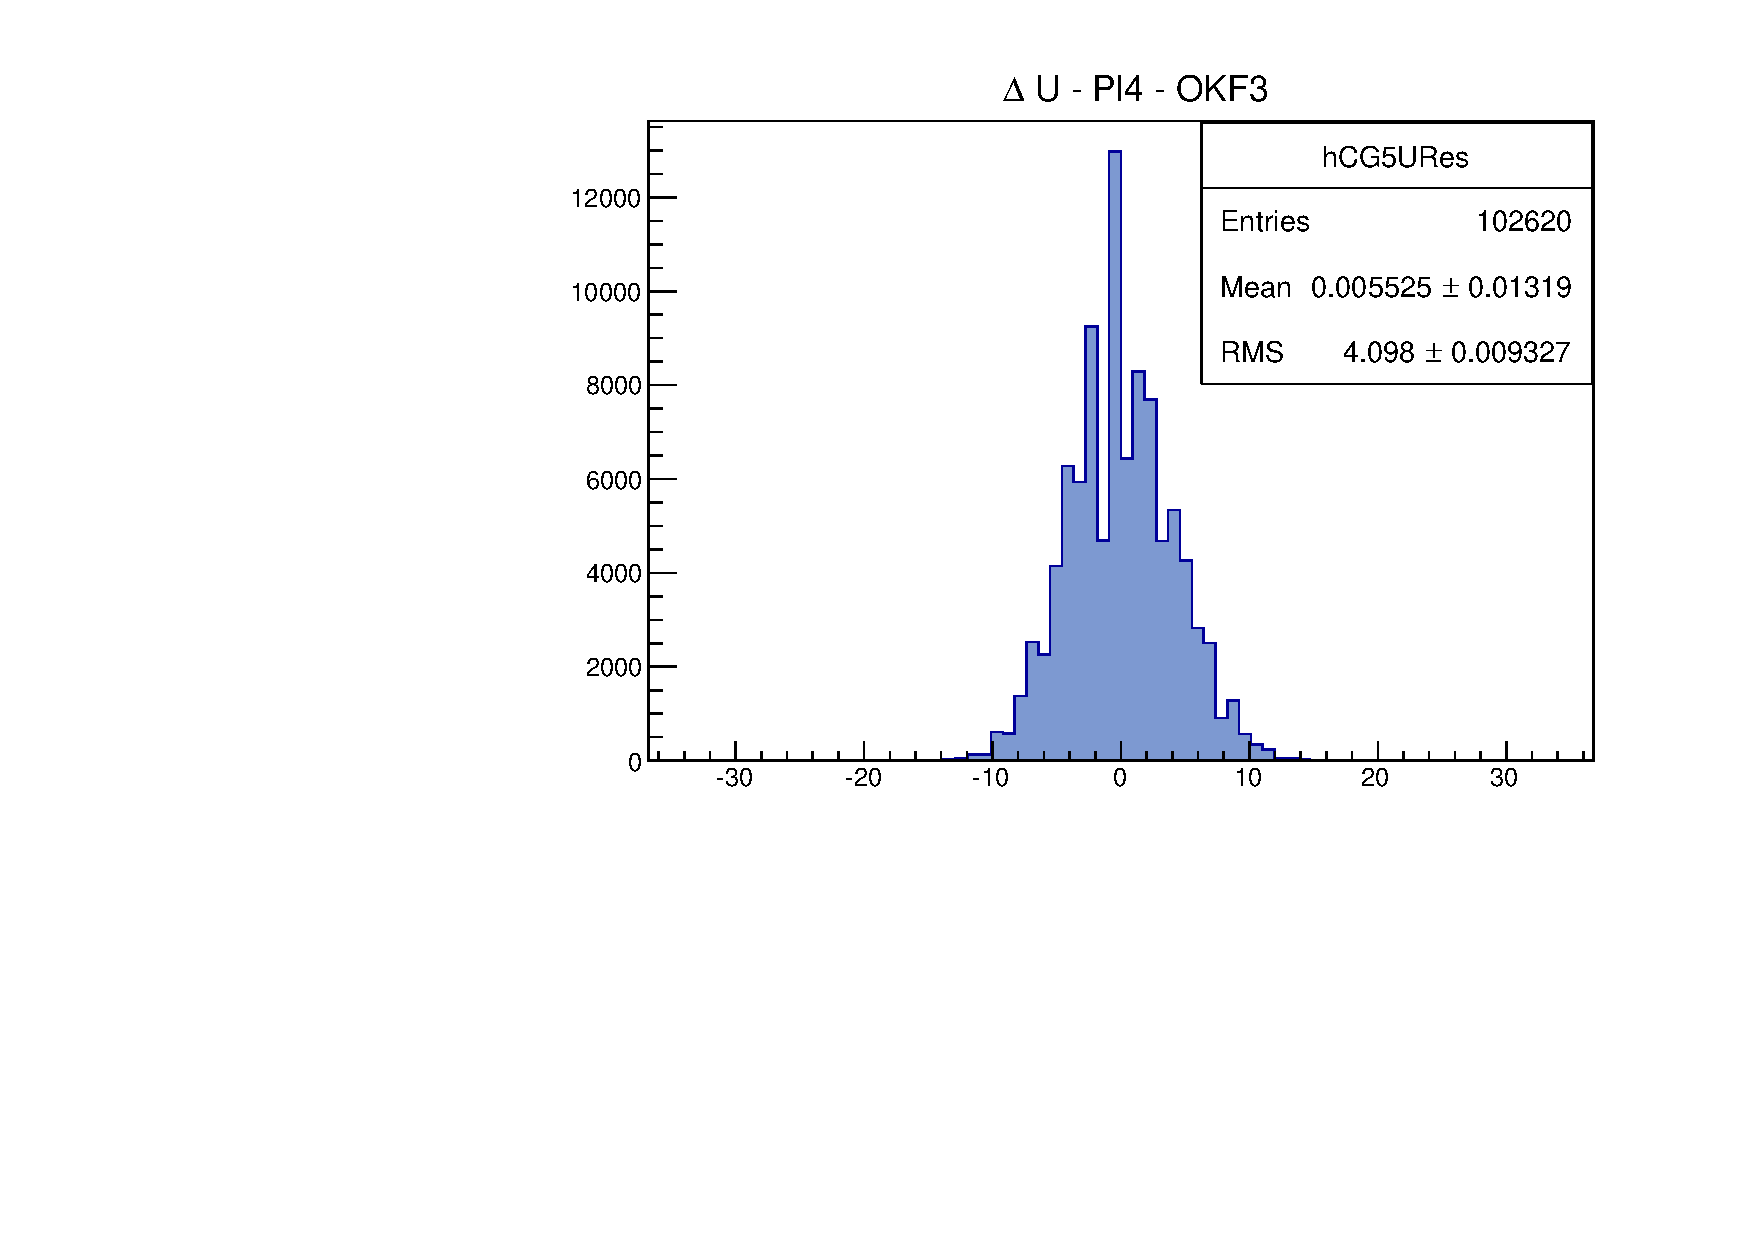
\includegraphics[scale=0.5]{./figures/Plots_PLUME/Alignement/ResU_DUT_PL4_OKF3.pdf}
     \caption{Distribution des r\'esidus sur le capteur 4 de la face OKF3. Le capteur est r\'egl\'e au seuil de $7 \, mV$.}
     \label{fig:alignDUT_PLUME}    
     \end{center}
   \end{figure}

  L'alignement des \textit{DUT}, c'est-\`a-dire des capteurs de l'\'echelle \textit{PLUME} est r\'ealis\'e avec une m\'ethode prenant en compte les six degr\'es de libert\'e du capteur consid\'er\'e. Par exemple, la figure \ref{fig:alignDUT_PLUME} illustre la distribution des r\'esidus selon l'axe horizontal $U$ du capteur 4 de la face \textit{OKF3}.
   
   \subsubsection{Homog\'en\'eit\'e de la r\'eponse}

   Les performances de chaque capteur de l'\'echelle PLUME ont \'et\'e test\'ees en terme d'efficacit\'e de d\'etection, de taux d'impacts fant\^omes, de multiplicit\'e des amas de pixels et de r\'esolution spatiale. Les r\'esultats pr\'esent\'es ici sont des r\'esultats datant de fin 2011 début 2012. D'autres analyses plus compl\`etes ont \'et\'e r\'ealis\'ees par la suite et d'autres sont encore en cours (fin 2014).
   
   
   
%   Pour la face \textit{OKF3} l'\'etape d'alignement n'a pu \^etre r\'ealis\'ee que pour les capteurs 1, 2, 4 et 5. Pour \textit{OKF6}, seuls les capteurs 2, 4 et 5 ont pu \^etre align\'es pr\'ecis\'ement. Plusieurs raisons peuvent \^etre avanc\'ees pour expliquer ces difficult\'es d'alignement. 
%    
%    \medskip
%    
%    !!!!!!!!!!!!!!! ICI !!!!!!!!!!!!!!!!!   
%    
%    Premi\`erement, la m\'ethode d'alignement automatique utilis\'ee n'a pas pu être utilis\'e pour effectu\'e un alignement. Sont en cause, un mauvais alignement nominal et un ............ Il a alors fallu aligner les capteurs en estimant leurs positions grossi\`erement puis en diminuant la valeur moyenne de la distribution des r\'esidus visible. En raison de la d\'eformation des capteurs sur l'\'echelle la distribution des r\'esidus s'en voit d\'eform\'ee. Cela augmente d'autant plus les difficult\'es d'alignement.

%    \medskip
%    
%    Plus le seuil est haut plus l'alignement est facile car moins de correlations ;) Ou pas ... ;p
%    OKF3
%    capteur3 -> pas assez de donn\'ees et alignement tres difficile.
%    capteur6 -> bad data.
%    OKF6
%    ?
%    ?
%    ///   METTRE PLOTS RESIDUS :)   ///
   
%    deformation des capteurs => distribution des residus non gaussienne et plus large.
%    Nombre d'impact par evt. --> correlations car pattern recognition difficile.
   
   \paragraph{Statistique et associations impacts-traces}
 
   La statistique utilis\'ee pour \'etablir les r\'esultats pr\'esent\'es pour l'\'echelle \textit{PLUME} est d'environ 40000 \'ev\'enements. Cela correspond \`a un nombre de traces plus \'elev\'ees. Pour nos analyses le nombre de traces maximum par \'ev\'enement a \'et\'e limit\'e \`a 30. Cependant, ce nombre important de traces est rarement atteint et on atteint en g\'en\'eral un nombre total de traces de l'ordre $10^5$, soit en moyenne environ 2 traces par \'ev\'enement. L'association des impacts sur les capteurs test\'es est r\'ealis\'ee en s\'electionnant l'impact le plus proche de l'extrapolation de la trace dans une fen\^etre de $100 \times 100 \mu m^2$ selon les axes $U$ et $V$ des capteurs.
   
   \paragraph{Unit\'e des seuils}
   
   Pour comparer les multiplicit\'es et les efficacit\'es obtenues sur chaque capteur analys\'e de l'\'echelle \textit{PLUME}, nous utiliserons des valeurs de seuil pour les discriminateurs en $mV$. En effet cette unit\'e est proportionnelle au signal r\'ecolté dans les pixels. Nous utiliserons aussi des seuils en $mV$ pour comparer les r\'esolutions spatiales des capteurs de l'\'echelle \textit{PLUME}. Cependant pour la comparaison des taux d'impacts fant\^omes, l'unit\'e naturelle pour le seuil des discriminateurs est le multiple du bruit moyen. Nous utiliserons donc cette unit\'e pour les analyses du taux d'impacts fant\^omes des capteurs analys\'es.
   
   \paragraph{Multiplicit\'e moyenne des amas}
   
%  \begin{landscape}
   
  \begin{figure}[htb!]
     \begin{center}
        \subfigure[Multiplicit\'es des amas de pixels pour les capteurs 1, 2, 4 et 5 de la face OKF3 de l'\'echelle PLUME en fonction du seuil des discriminateurs en $mV$.]{
            \label{fig:mult_OKF3}
            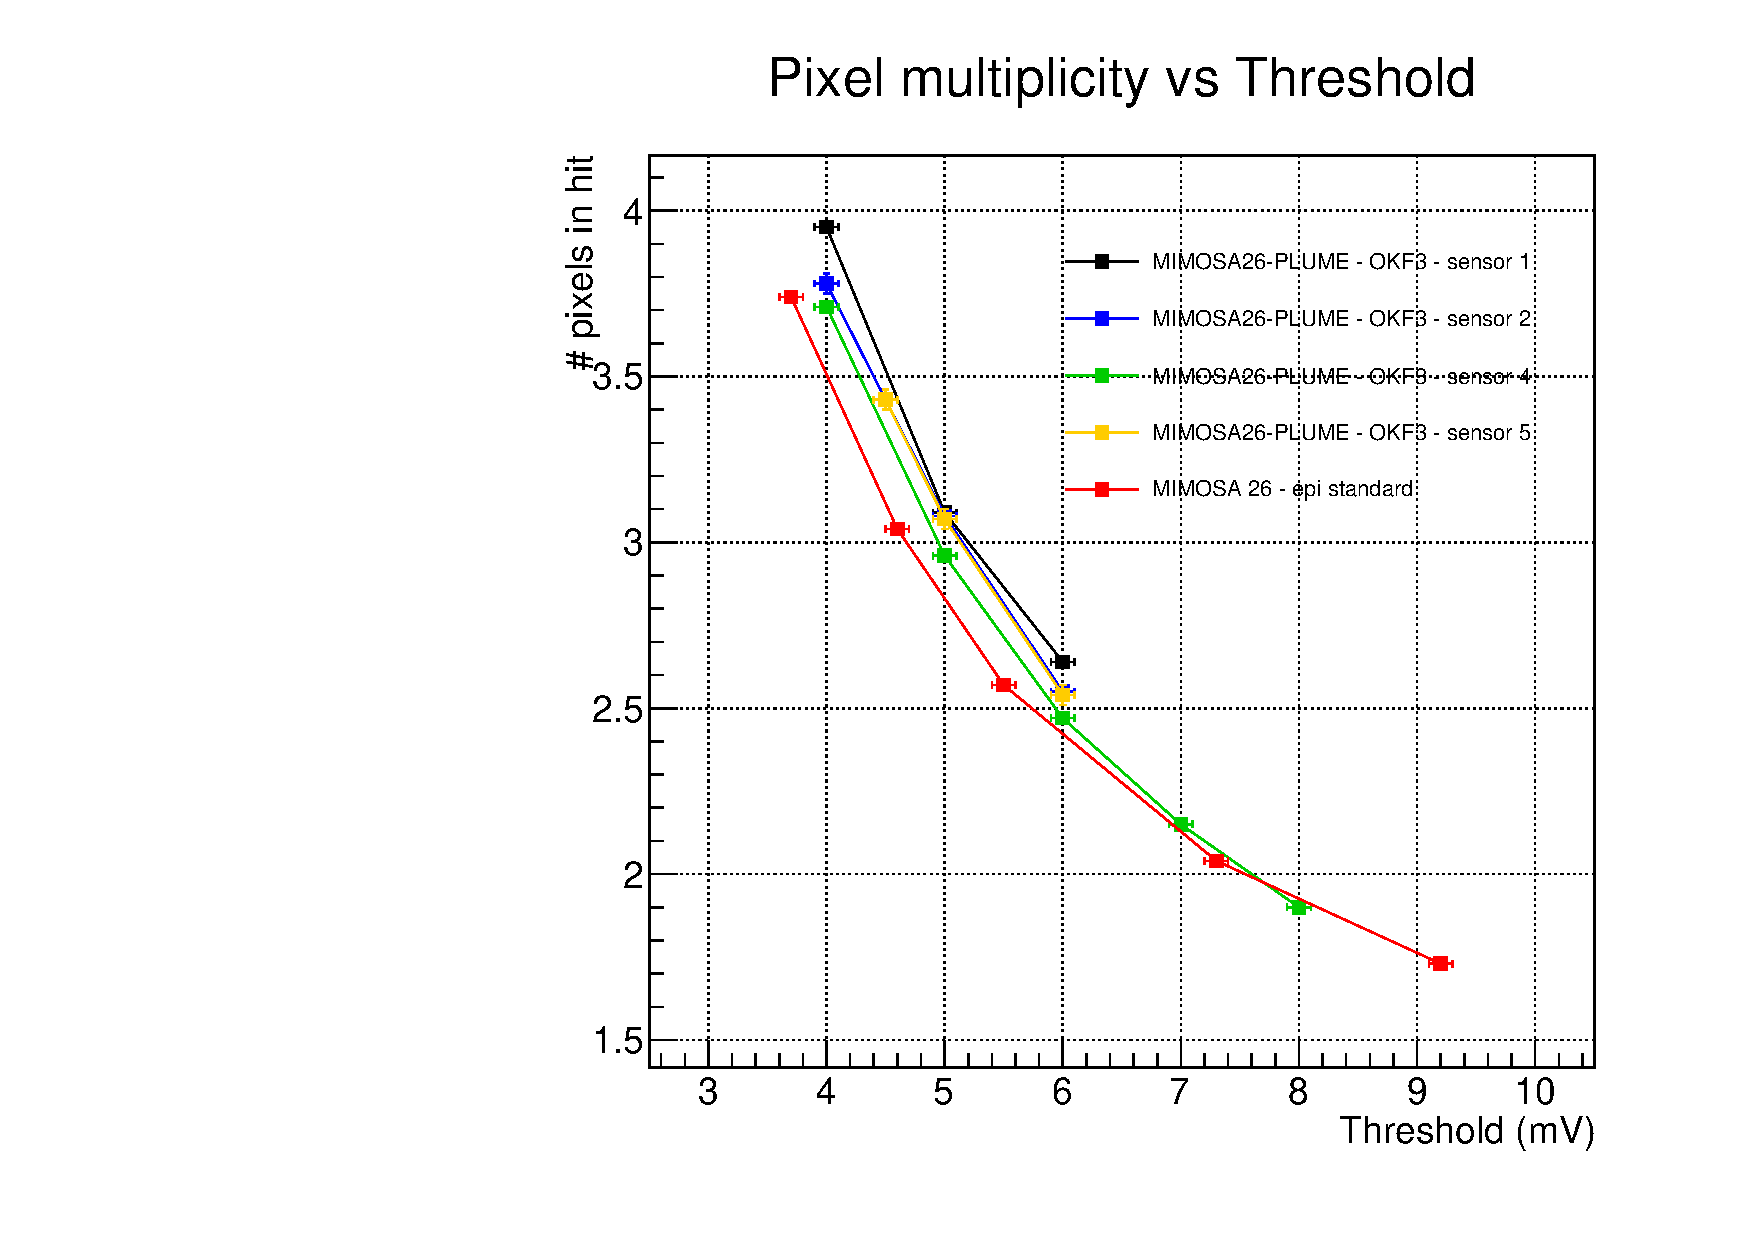
\includegraphics[width=0.47\textwidth]{./figures/Plots_PLUME/OKF3_Mult_Thr_mV.pdf}
        }
        \subfigure[Multiplicit\'e des amas de pixels des capteurs de la face OKF6 en fonction du seuil des discriminateurs en $mV$.]{
           \label{fig:mult_OKF6}
           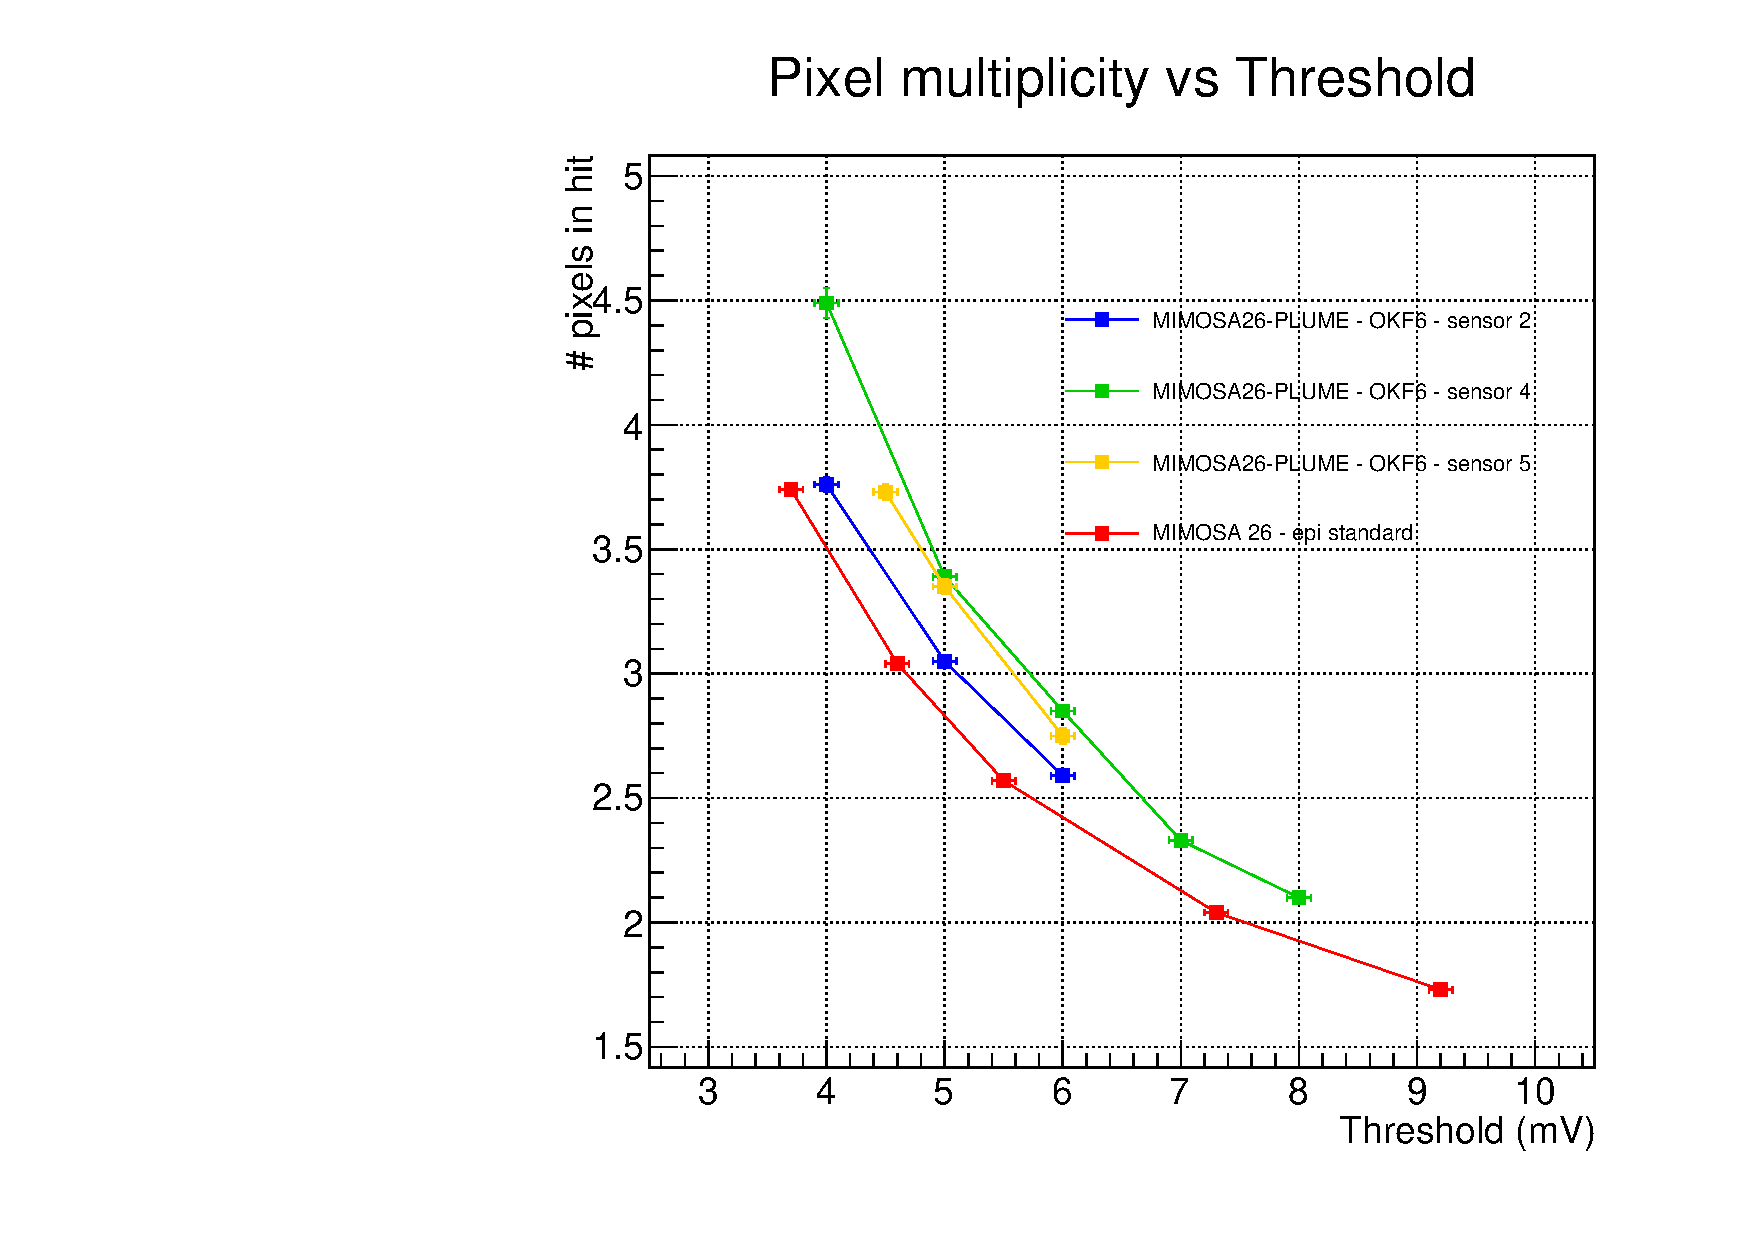
\includegraphics[width=0.47\textwidth]{./figures/Plots_PLUME/OKF6_Mult_Thr_mV.pdf}
        }
     \end{center}
     \caption{Multiplicit\'e des amas de pixels des capteurs composant l'\'echelle PLUME, compar\'ees avec la multiplicit\'e du capteur de r\'ef\'erence MIMOSA-26 (en rouge).}
     \label{fig:mult_PLUME}
   \end{figure}
   
%   \end{landscape}
  
   Les figures \ref{fig:mult_OKF3} et \ref{fig:mult_OKF6} repr\'esentent les multiplicit\'es moyennes des amas de pixels en fonction du seuil des discriminateurs en $mV$ pour les six capteurs de la face \textit{OKF3} et les six autres capteurs de la face \textit{OKF6}. Ces multiplicit\'es sont compar\'ees \`a celles du capteur de r\'ef\'erence MIMOSA-26. Sur les deux faces des capteurs, les multiplicit\'es mesur\'ees \`a bas seuil (entre 4 et $6 \, mV$) sont plus \'elev\'ees que celles du capteur de r\'ef\'erence r\'egl\'e au m\^eme seuil. 
   
   \medskip
   
   Sur la face \textit{OKF3} on observe des multiplicit\'es moyennes environ $10 \%$ plus \'elev\'ees que le capteur de r\'ef\'erence. Pour cette face, le capteur 1 a la plus haute multiplicit\'e moyenne. Pour ce capteur on passe ainsi de 3.95 pixels par amas en moyenne \`a 2.65 pixels par amas entre les seuils de 4 \`a 6 $mV$, ce qui correspond \`a des valeurs de multiplicit\'es moyennes plus \'elev\'ees d'environ 15 \`a 10\% par rapport au capteur de r\'ef\'erence. Les capteurs 2 et 5 de la face \textit{OKF3} arborent la m\^eme multiplicit\'e moyenne. On passe ainsi de 3.8 \`a 2.55 pixels par amas en moyenne pour des seuils variant entre 4 et 6 $mV$. Cela correspond \`a une augmentation d'environ respectivement 10\% \`a 5\%. Enfin pour le capteur 4 de la face \textit{OKF3} la multiplicit\'e moyenne varie entre 3.7 et 1.9 pixels par amas pour des seuils variant de 4 \`a 8 $mV$. Pour ce capteur, les multiplicit\'es mesur\'ees correspondent \`a celles du capteur de r\'ef\'erence pour des seuils de 7 et 8 $mV$, puis \`a plus bas seuil la multiplicit\'e obtenue est plus \'elev\'ee. On atteint ainsi un \'ecart maximal d'environ +5\% au seuil de 4 $mV$. 
   
   \medskip
   
   Pour la face \textit{OKF6}, les multiplicit\'es moyennes sont aussi plus \'elev\'ees. Les capteurs 4 et 5 de la face \textit{OKF6} pr\'esentent une multiplicit\'e moyenne similaire. Ainsi on passe de 4.5 pixels par amas en moyenne au seuil de $4 \, mV$ \`a 2.1 pixels par amas au seuil de $8 \, mV$. Cela correspond \`a des augmentations de multiplicit\'e variant entre $30\%$ au seuil de $4 \, mV$ \`a 10\% au seuil de $8 \, mV$. Enfin, le capteur 2 de la face \textit{OKF6} poss\`edent une multiplicit\'e variant entre 3.75 et 2.6 pixels par amas en moyenne entre les seuils de 4 et $6 \, mV$. Cela correspond \`a une augmentation variant d'environ $7\%$ entre les seuils de 4 et $6 \, mV$.  
   
   \medskip

   Ainsi, les multiplicit\'es moyennes observ\'ees sur les capteurs de l'\'echelle \textit{PLUME} sont plus \'elev\'ees que celles du capteur de r\'ef\'erence. L'augmentation des multiplicit\'es obtenues varie en fonction du capteur \'etudi\'e et du seuil appliqu\'e. Cela laisse penser que le signal est plus ou moins fort selon le capteur. En effet, si le signal est plus \'elev\'e compar\'e au capteur de r\'ef\'erence, cela signifie que plus de charges arrivent au niveau des pixels. Ainsi, \`a seuil de discriminiteurs identique plus de pixels passent le seuil. Cela se traduit par des multiplicit\'es et des efficacit\'es de d\'etection plus \'elev\'ees. Si tel \'etait le cas cela pourrait signifier des diff\'erences de calibration du gain entre les capteurs. Pour confirmer ce fait, on pourra se r\'ef\'erer aux valeurs des efficacit\'es obtenues. Nous allons donc \'etudier les efficacit\'es de d\'etection au regard de ces observations.
   
   \paragraph{Efficacit\'e de d\'etection}
   
   Nous allons ici discuter les efficacit\'es de d\'etection obtenues sur chacun des capteurs de l'\'echelle \textit{PLUME} analys\'es. Nous allons orienter notre discussion en fonction des diff\'erences de multiplicit\'es observ\'ees afin de v\'erifier si ici aussi une diff\'erence entre les gains de capteurs est visible. Pour comparer ces r\'esultats au capteur MIMOSA-26 de r\'ef\'erence on insistera sur le fait que la fen\^etre temporelle DUT/t\'elescope pour calculer les efficacit\'es de ce capteur a \'et\'e \'etendue afin de maximiser les valeurs d'efficacit\'e obtenues. Cette op\'eration n'a pas \'et\'e r\'ealis\'ee sur les capteurs de l'\'echelle \textit{PLUME}. Ainsi, pour les capteurs de l'\'echelle \textit{PLUME}, on s'attend \`a des efficacit\'es tr\`es l\'eg\`erement inf\'erieures au capteur de r\'ef\'erence. Les figures \ref{fig:efficiency_OKF3} et \ref{fig:efficiency_OKF6} montrent les efficacit\'es de d\'etection obtenues sur chacun des capteurs test\'es des faces \textit{OKF3} et \textit{OKF6} en fonction du seuil en $mV$ des discriminateurs de chacun de ces capteurs.

%  \begin{landscape}
  
  \begin{figure}[htb!]
     \begin{center}
        \subfigure[Efficacit\'e de d\'etection pour les capteurs de la face OKF3 en fonction du seuil des discriminateurs en $mV$.]{
            \label{fig:efficiency_OKF3}
            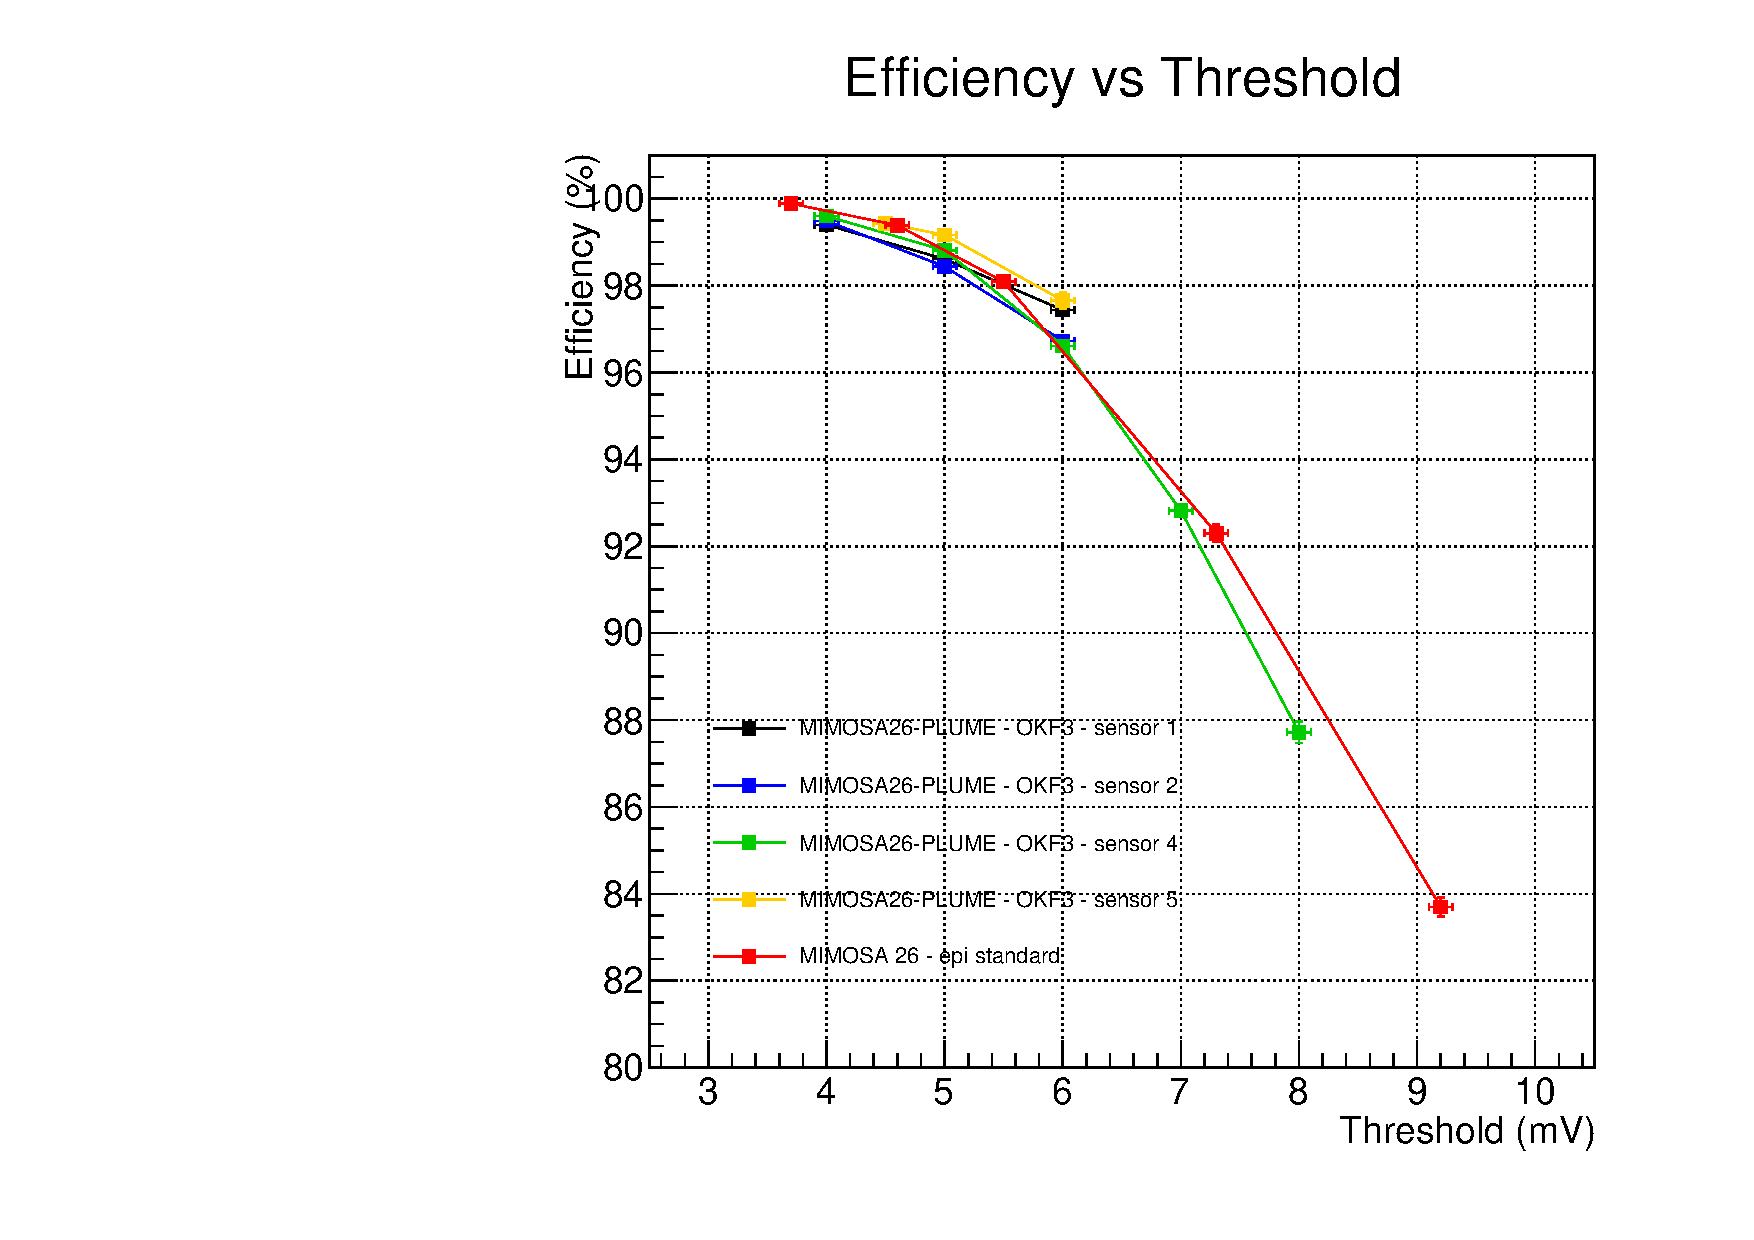
\includegraphics[width=0.47\textwidth]{./figures/Plots_PLUME/OKF3_Eff_Thr_mV.pdf}
        }
        \subfigure[Efficacit\'e de d\'etection pour les capteurs de la face OKF6 en fonction du seuil des discriminateurs en $mV$.]{
           \label{fig:efficiency_OKF6}
           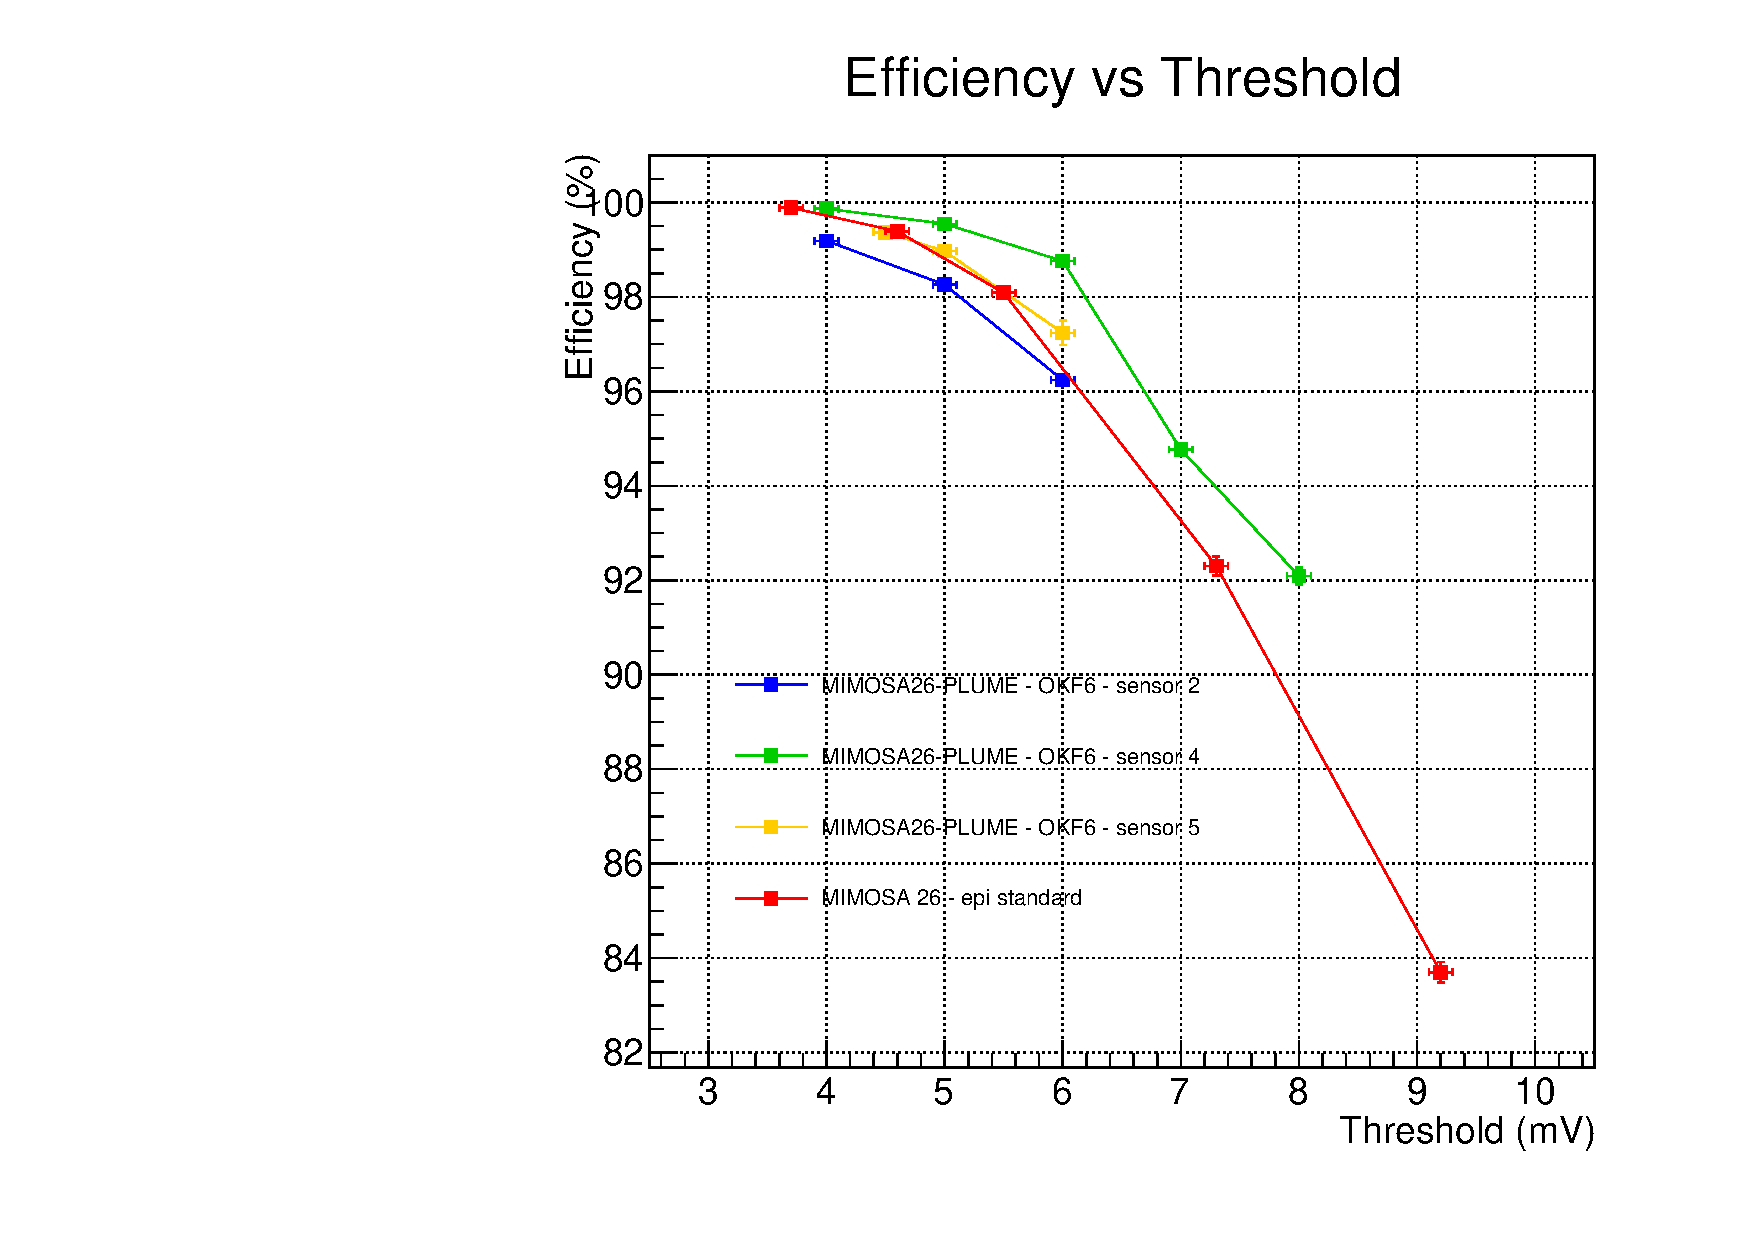
\includegraphics[width=0.47\textwidth]{./figures/Plots_PLUME/OKF6_Eff_Thr_mV.pdf}
        }
     \end{center}
     \caption{Efficacit\'e des capteurs composant l'\'echelle PLUME, compar\'ees avec l'efficacit\'e du capteur de r\'ef\'erence MIMOSA-26 (en rouge).}
     \label{fig:mult_PLUME}
   \end{figure} 

%   \end{landscape}

   \medskip
   
   Pour la face \textit{OKF3} on observe des efficacit\'es de d\'etection proches de celles du capteur de r\'ef\'erence. Pour les capteurs 2 et 4 de cette face, les efficacit\'es sont l\'eg\`erement au dessous de celles du capteur de r\'ef\'erence comme attendu. On passe ainsi d'environ 99.5\% d'efficacité au seuil de 4 $mV$ \`a environ 87.5\% au seuil de 8 $mV$. Pour le capteur 1 de \textit{OKF3} l'efficacité varie de environ $99.5$ \`a $98.75\%$ pour des seuils de 4 \`a $5 \, mV$. Ces efficacit\'es sont tr\`es l\'eg\`erement inf\'erieures \`a celles du capteur de r\'ef\'erence. Puis pour un seuil de 6 $mV$ l'efficacit\'e devient supérieure \`a celle du capteur de r\'ef\'erence puisqu'elle atteint environ 97.5\% compar\'e au 96.5\% du capteur de r\'ef\'erence. Même si cette augmentation est inf\'erieure au \% une variation de l'ordre de 0.5\% est significative lorsque les efficacit\'es approchent des 100\%. L'efficacit\'e du capteur 5 de la face \textit{OKF3} est quant \`a elle \'egale au capteur de r\'ef\'erence au seuil de 4.5 mV puisqu'elle atteint environ 99.5\% et sup\'erieure \`a la r\'ef\'erence pour des seuils de 5 et $6 \, mV$. Les efficacit\'es respectivement atteintes sont d'environ 99.25\% et 97.75\%. Ces valeurs sont \`a comparer aux valeurs d'environ 98.5\% et 96.75\% pour le capteur de r\'ef\'erence aux m\^emes seuils. 
   
   \medskip
   
   Pour les capteurs 1, 2 et 5, on observe des valeurs d'efficacit\'es inf\'erieures o\`u \'egales au capteur de r\'ef\'erence \`a bas seuil , puis pour des valeurs de seuils plus \'elev\'ees les efficacit\'es deviennent sup\'erieures ou \'egales \`a celles du capteur de r\'ef\'erence. Ce comportement pourrait s'expliquer par la saturation de la m\'emoire par les lignes ou les colonnes bruyantes. En effet, plus le seuil est bas plus la saturation des m\'emoires est importante et plus le seuil est haut, plus cette saturation diminue. Une saturation de la m\'emoire implique une perte de certains impacts et donc une moins bonne efficacit\'e de d\'etection. Ainsi, \`a bas seuil on observe des efficacit\'es moins \'elev\'ees. Puis plus le seuil augmente plus l'efficacit\'e augmente et devient sup\'erieure \`a celle du capteur de r\'ef\'erence. De plus, si l'on conjugue cette explication avec la prise en compte de la plus haute efficacit\'e attendue pour le capteur de r\'ef\'erence d\^u \`a l'extension de la fen\^etre temporelle, on observe un l\'eger d\'ecalage des courbes d'efficacit\'e vers les seuils plus \'elev\'es. Ce d\'ecalage est alors compatible avec la hausse de la multiplicit\'e observ\'ee pr\'ec\'edemment. Un signal plus \'elev\'e serait donc responsable des diff\'erences observ\'ees. De plus, un calibrage l\'eg\`erement diff\'erent du gain des capteurs expliquerait les variabilit\'es des multiplicit\'es et des efficacit\'es obtenues. 
   
   \medskip
   
   Pour la face \textit{OKF6} les diff\'erences d'efficacit\'es sont plus marqu\'ees. Le capteur 4 de cette face pr\'esente des efficacit\'es de 99.9\%, 98.75\% et 92\% pour des seuils de respectivement $4 \, mV$, $6 \, mV$ et $8 \, mV$. Ces efficacit\'es sont plus \'elev\'ees que celles du capteur de r\'ef\'erence qui pr\'esente des efficacit\'es d'environ 99.5\%, 96.25\% et 89\% aux m\^emes seuils. Le capteur 5 de cette face pr\'esente les m\^emes valeurs d'efficacit\'es que le capteur de r\'ef\'erence pour des seuils de $4.5$ et $5 \, mV$. Puis au dessus du seuil de $5\, mV$ l'efficacit\'e est plus haute que celle du capteur de r\'ef\'erence. Elle atteint ainsi 97.25\% au seuil de $6 \, mV$ pour une valeur d'efficacit\'e du capteur de r\'ef\'erence au m\^eme seuil d'environ 96.25\%. enfin le capteur 2 de cette face pr\'esente des efficacit\'es inf\'erieures au capteur de r\'ef\'erence. Pour ce capteur, on passe ainsi d'une efficacit\'e de 99.2\% au seuil de $4 \, mV$ \`a 96.25 \% au seuil de $6 \, mV$. Toutefois plus le seuil augmente plus la diff\'erence avec le capteur de r\'ef\'erence diminue. On peut alors supposer qu'à plus haut seuil, l'efficacit\'e sur ce capteur d\'epasse celle du capteur de r\'ef\'erence. Les diff\'erences observ\'ees pour cette face s'expliquent aussi par la saturation des m\'emoires \`a bas seuils coupl\'ee \`a une l\'eg\`ere variabilit\'e du calibrage du gain des capteurs.

   \paragraph{R\'esolution spatiale}
   
   Dans cette partie nous allons discuter les r\'esolutions spatiales obtenues sur les capteurs de l'\'echelle \textit{PLUME} test\'ee. Tout d'abord, des diff\'erences dans les distributions de multiplicit\'es pour chaque capteur et pour chaque seuil on \'et\'e observ\'ees. De fa\c{c}on g\'en\'erale, les r\'esolutions spatiales obtenues pour des multiplicit\'es d'amas de 1, 2, 3, 4 ou 5 pixels diff\`erent en raison d'un centre de gravit\'e plus ou moins bon selon la forme de l'amas de pixels. Ainsi, \'etant donn\'e le pas inter-pixel et le m\'elange de toutes les formes d'amas, on obtient une distribution des r\'esidus sur le \textit{DUT} consid\'er\'e plus ou moins large. Il est donc difficile de d\'ecrire le comportement de la r\'esolution spatiale obtenue sur chacun des capteurs analys\'es de l'\'echelle \textit{PLUME} sans \'etudier les distributions de multiplicit\'es. Cependant, dans ce paragraphe, nous ne d\'ecrirons essentiellement que les \'ecarts et l'homog\'en\'eit\'e de la r\'esolution spatiale obtenue sur les diff\'erents capteurs test\'es de l'\'echelle \textit{PLUME} mise en faisceau compar\'es au capteur MIMOSA-26 de r\'ef\'erence.
   
   \medskip
   
%   \begin{landscape}
  
  \begin{figure}[htb!]
     \begin{center}
        \subfigure[R\'esolution spatiale des capteurs de la face \textit{OKF3} en fonction du seuil des discriminateurs en $mV$.]{
            \label{fig:resolution_OKF3}
            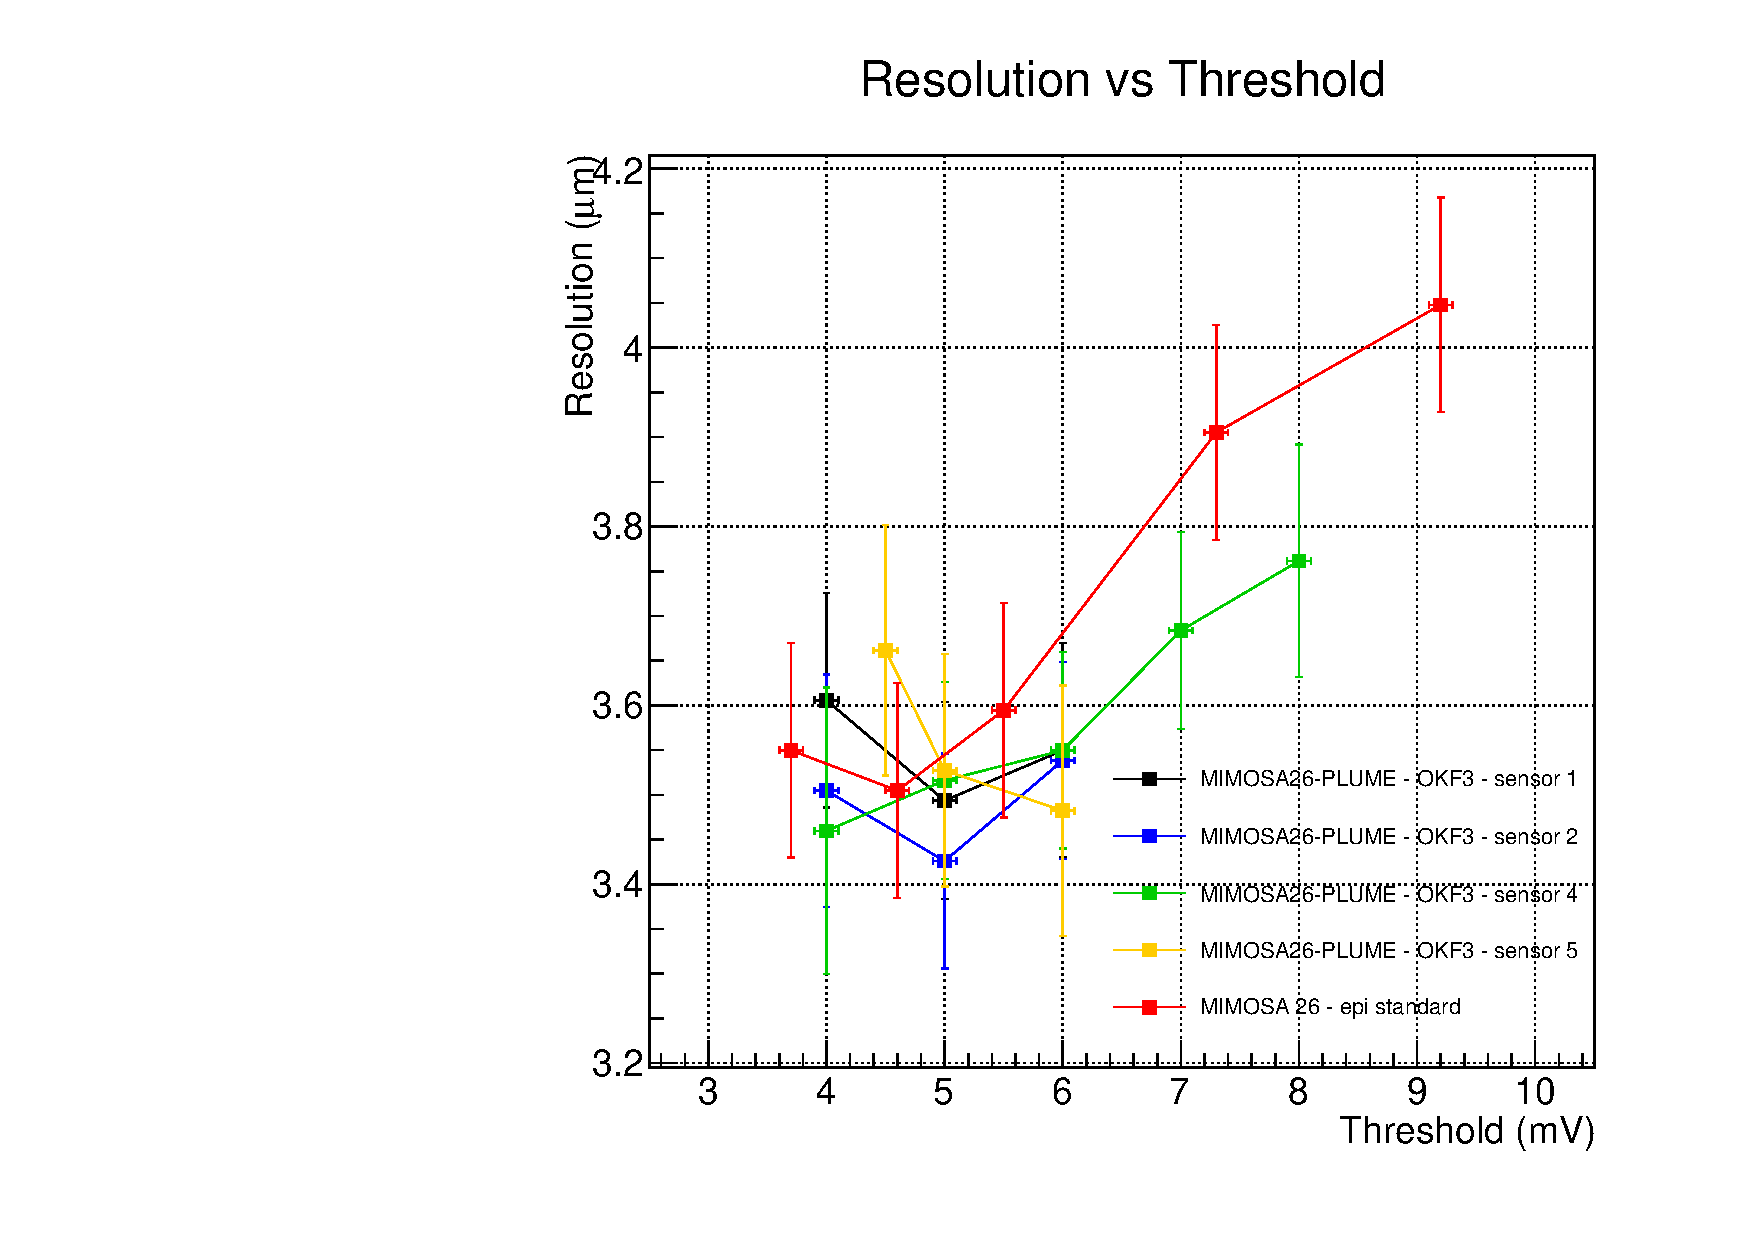
\includegraphics[width=0.47\textwidth]{./figures/Plots_PLUME/OKF3_Res_Thr_mV.pdf}
        }
        \subfigure[R\'esolution spatiale des capteurs de la face \textit{OKF6} en fonction du seuil des discriminateurs en $mV$.]{
            \label{fig:resolution_OKF6}
            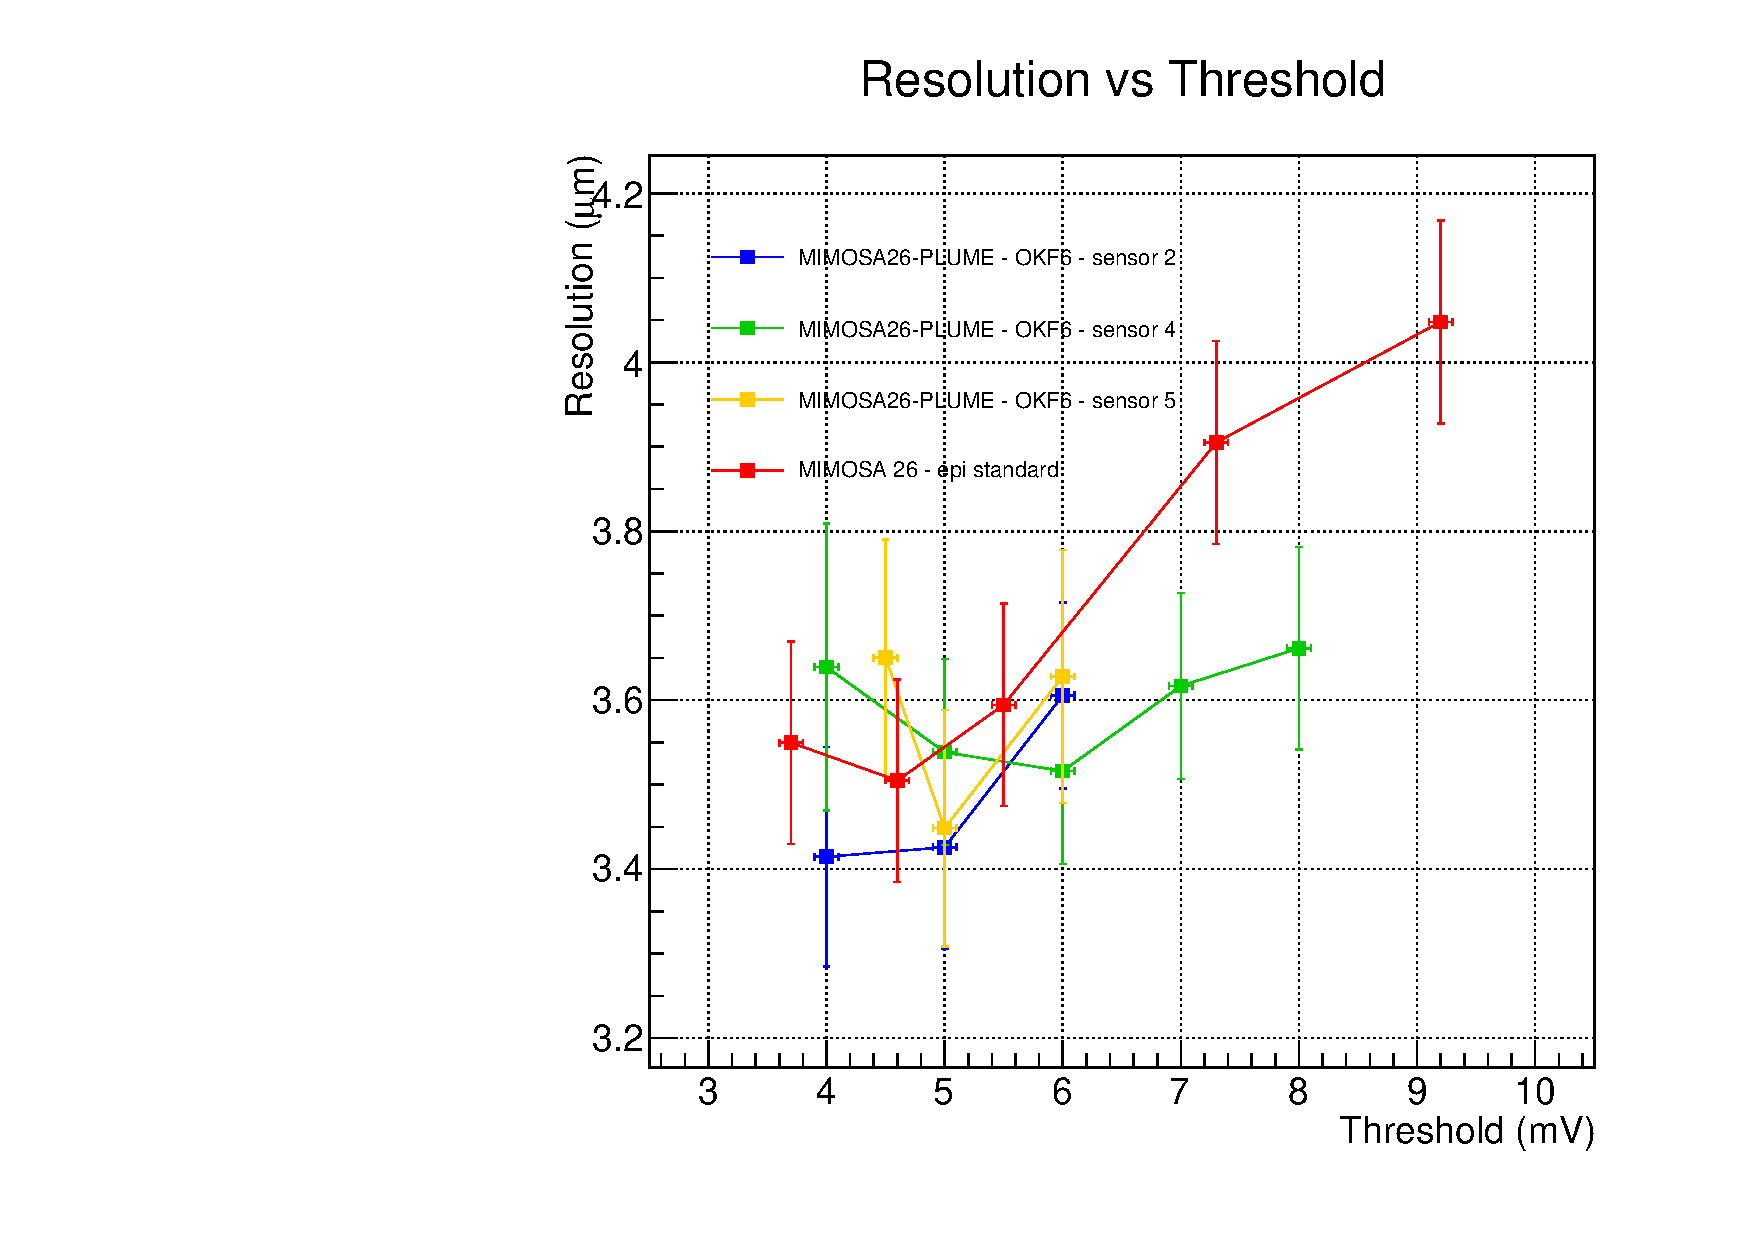
\includegraphics[width=0.47\textwidth]{./figures/Plots_PLUME/OKF6_Res_Thr_mV.pdf}
        }
     \end{center}
     \caption{R\'esolution spatiale des capteurs composant l'\'echelle PLUME, compar\'ees avec le taux d'impacts fant\^omes du capteur de r\'ef\'erence MIMOSA-26 (en rouge).}
     \label{fig:resol_PLUME}
   \end{figure} 

%   \end{landscape}
   
   Afin d'extraire les r\'esolutions spatiales sur les diff\'erents capteurs, les largeurs des distributions des r\'esidus $\sigma_{Res}$ obtenues sur chacun des capteurs ont \'et\'e extraites. La r\'esolution du capteur consid\'er\'e est calcul\'ee grâce \`a la relation \ref{eq:resolution} en prenant en compte la r\'esolution du t\'elescope de $\sigma_{Tel}$ et une diffusion multiple n\'egligeable c'est-à-dire $\sigma_{ms} = 0$. On a alors :
   
   \begin{equation}
    \sigma_{DUT} = \sqrt{\sigma_{Res}^2 - \sigma_{Tel}^2}
   \end{equation}

   Les calculs de la r\'esolution spatiale sur les capteurs sont sensibles \`a la r\'esolution du t\'elescope et donc \`a son alignement. On notera que comme l'\'echelle n'est pas exactement centr\'ee au centre du t\'elescope, la valeur de la r\'esolution du télescope n'est pas exactement la m\^eme au niveau des deux faces de l'\'echelle. Les deux valeurs de r\'esolution du t\'elescope calcul\'ees pour chacune des faces valent environ $1.806 \, \mu m$ et $1.801$. La diff\'erence est infime et on prend $\sigma_{Tel} = 1.8 \mu m$. Une incertitude syst\'ematique de $0.1 \, \mu m$ repr\'esentant entre autres les incertitudes sur la diffusion multiple cr\'ee par le support de l'\'echelle PLUME et la r\'esolution du t\'elescope a \'et\'e ajout\'ee aux valeurs de r\'esolutions spatiales obtenues.
   
   \medskip
   
   Les figures \ref{fig:resolution_OKF3} et \ref{fig:resolution_OKF6} illustrent les r\'esolutions spatiales obtenues sur chacun des capteurs test\'es en fonction du seuil de fonctionnement des discriminateurs en $mV$. Sur ces deux faces, les r\'esolutions spatiales mesur\'ees sont similaires \`a celles du capteur MIMOSA-26 de r\'ef\'erence aux incertitudes pr\`es. Les r\'esolutions minimales obtenues atteignent la valeur de $3.5 \pm 0.1 \, \mu m$. Elles sont obtenues pour des seuils compris entre 4 et $6 \, mV$. Cela s'explique par les diff\'erences de multiplicit\'es moyennes observ\'ees. Toutefois comme les distributions de multiplicit\'es peuvent varier \`a moyennes identiques, nous ne pouvons d\'ecrire les diff\'erences obtenues qu'en vertu des distributions de multiplicit\'es. Ainsi, nous ne commenterons pas plus ces r\'esultats.

   \paragraph{Taux d'impacts fant\^omes}
   
   Le dernier param\`etre cl\'e permettant de caract\'eriser un capteur CMOS est le taux d'impacts fant\^omes. Ce taux est calcul\'e avec les capteurs de l'\'echelle hors faisceau. Le calcul a \'et\'e r\'ealis\'e en consid\'erant une seule trame par \'ev\'enement et en utilisant une zone rectangulaire prise entre les points extr\^emes $(-3000,-3000)$ et $(3000,4000)$ selon les coordonn\'ees $(U,V)$ des capteurs.
   
   \medskip
   
   Comme nous l'avons vu, l'unit\'e naturelle pour comparer le taux d'impacts fant\^omes est le multiple du bruit moyen. Les figures \ref{fig:fantomes_OKF3} et \ref{fig:fantomes_OKF6} pr\'esentent les taux d'impacts fant\^omes obtenus en fonction du seuil exprim\'e en multiple du bruit moyen de chaque capteur. Sur ces figures on observe des taux d'impacts fant\^omes pour les capteurs de l'\'echelle \textit{PLUME} inf\'erieurs jusqu'à un ordre de grandeur compar\'e au capteur MIMOSA-26 de r\'ef\'erence. Les taux d'impacts fant\^omes mesur\'es sont alors inf\'erieurs \`a $2 \times 10^{-4}$ au seuil de 4 fois le bruit moyen. De plus le taux d'impacts fant\^omes varie en fonction du capteur test\'e. 
   
   \medskip
   
%  \begin{landscape}
 
  \begin{figure}[htb!]
     \begin{center}
        \subfigure[Taux d'impacts fant\^omes des capteurs de la face OKF3 en fonction du seuil des discriminateurs en multiple du bruit moyen.]{
            \label{fig:fantomes_OKF3}
            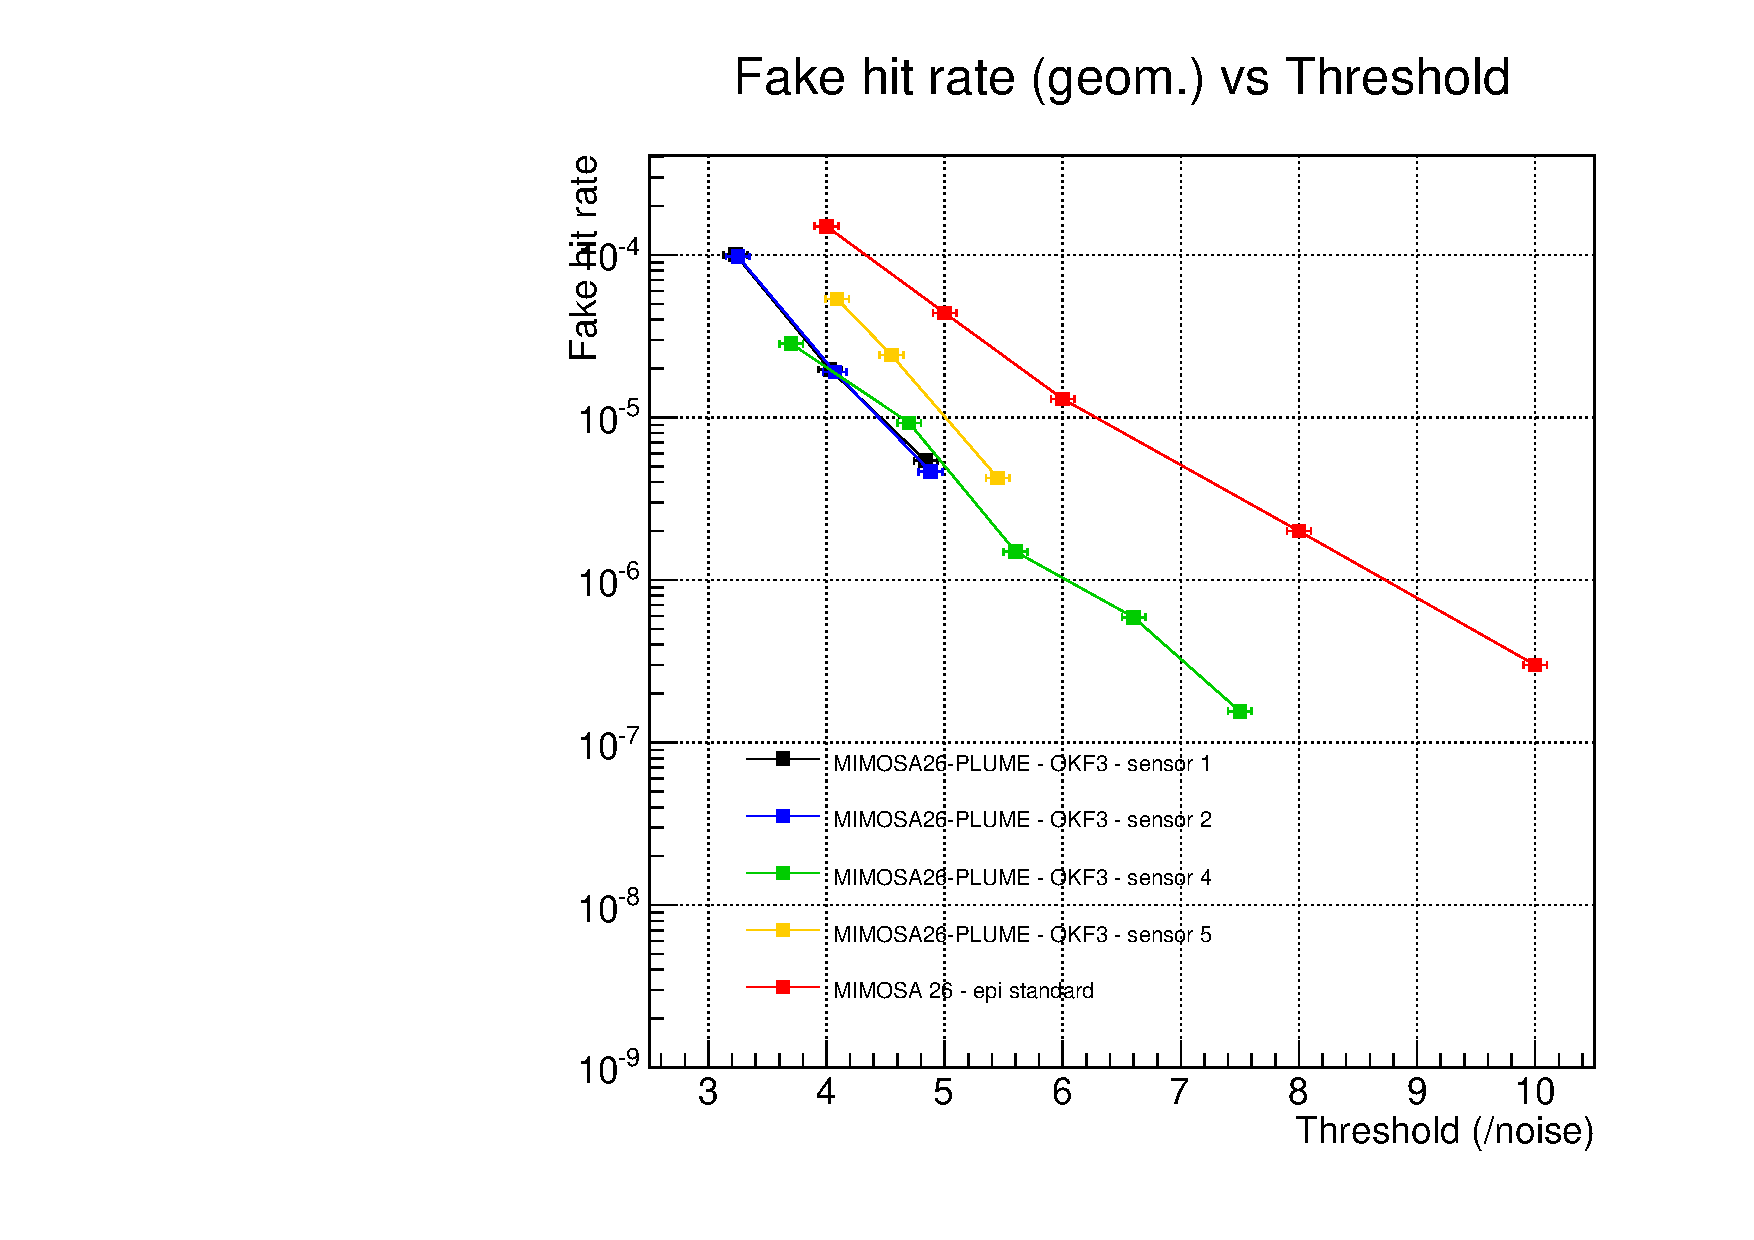
\includegraphics[width=0.46\textwidth]{./figures/Plots_PLUME/OKF3_Fake_Thr_noise.pdf}
        }
        \subfigure[Taux d'impacts fant\^omes des capteurs de la face OKF6 en fonction du seuil des discriminateurs en multiple du bruit moyen.]{
            \label{fig:fantomes_OKF6}
            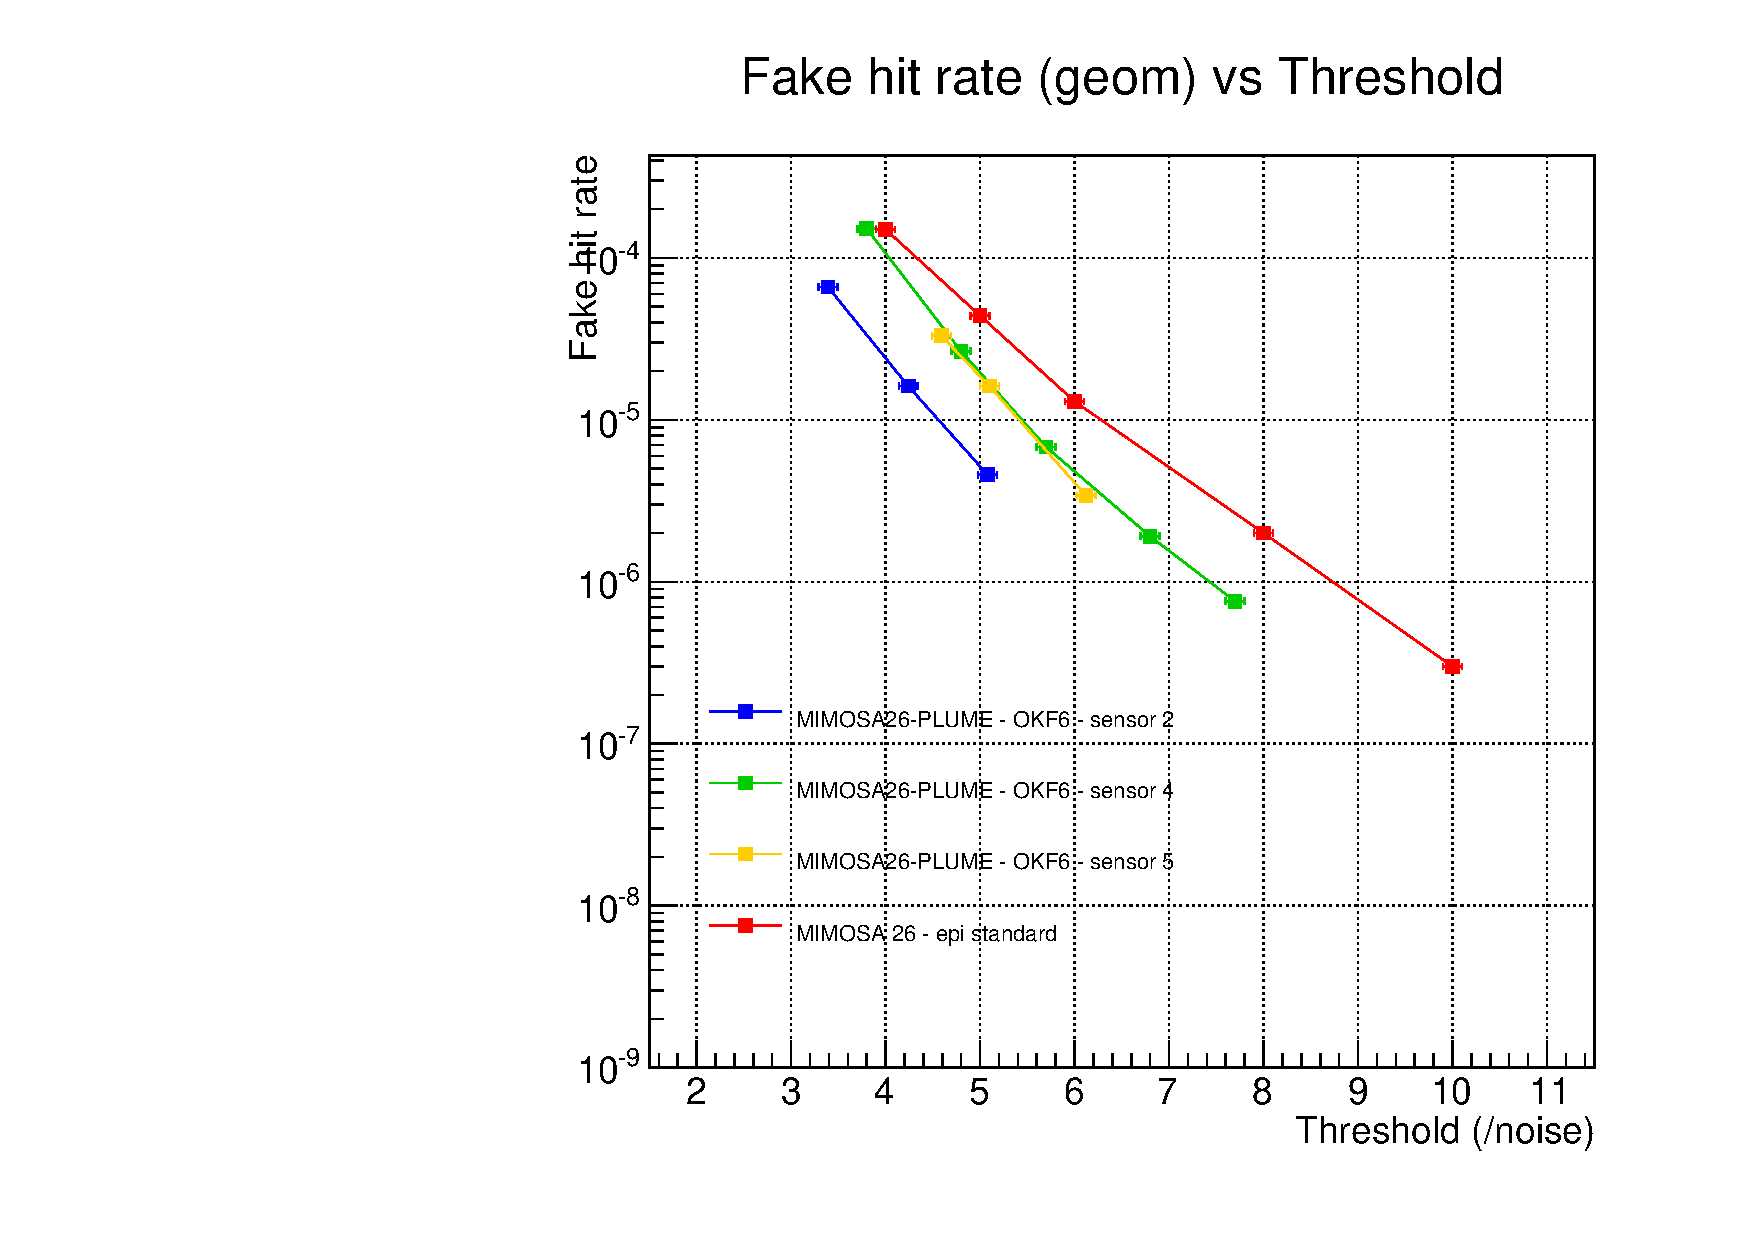
\includegraphics[width=0.46\textwidth]{./figures/Plots_PLUME/OKF6_Fake_Thr_noise.pdf}
        }
     \end{center}
     \caption{Taux d'impacts fant\^omes en fonction du seuil appliqu\'e pour les capteurs composant l'\'echelle PLUME, compar\'es avec les taux d'impacts fant\^omes du capteur de r\'ef\'erence MIMOSA-26 (en rouge).}
     \label{fig:fantomes_PLUME}
   \end{figure} 

%   \end{landscape}
   
   Pour expliquer ces r\'esultats, on rappelle que le taux d'impacts fant\^omes est domin\'e par un nombre de pixels $\lesssim 1\%$ plus bruyants que les autres. On peut supposer que ce nombre de pixels plus bruyants fluctue selon l'exemplaire de capteur test\'e puisqu'il d\'epend directement de la variabilit\'e de fabrication du capteur. Ainsi, les diff\'erences obtenues signent un faible taux de pixels plus bruyants que les autre.
   
   \FloatBarrier
   
%    \begin{figure}[!htb]
%    \begin{center}
%     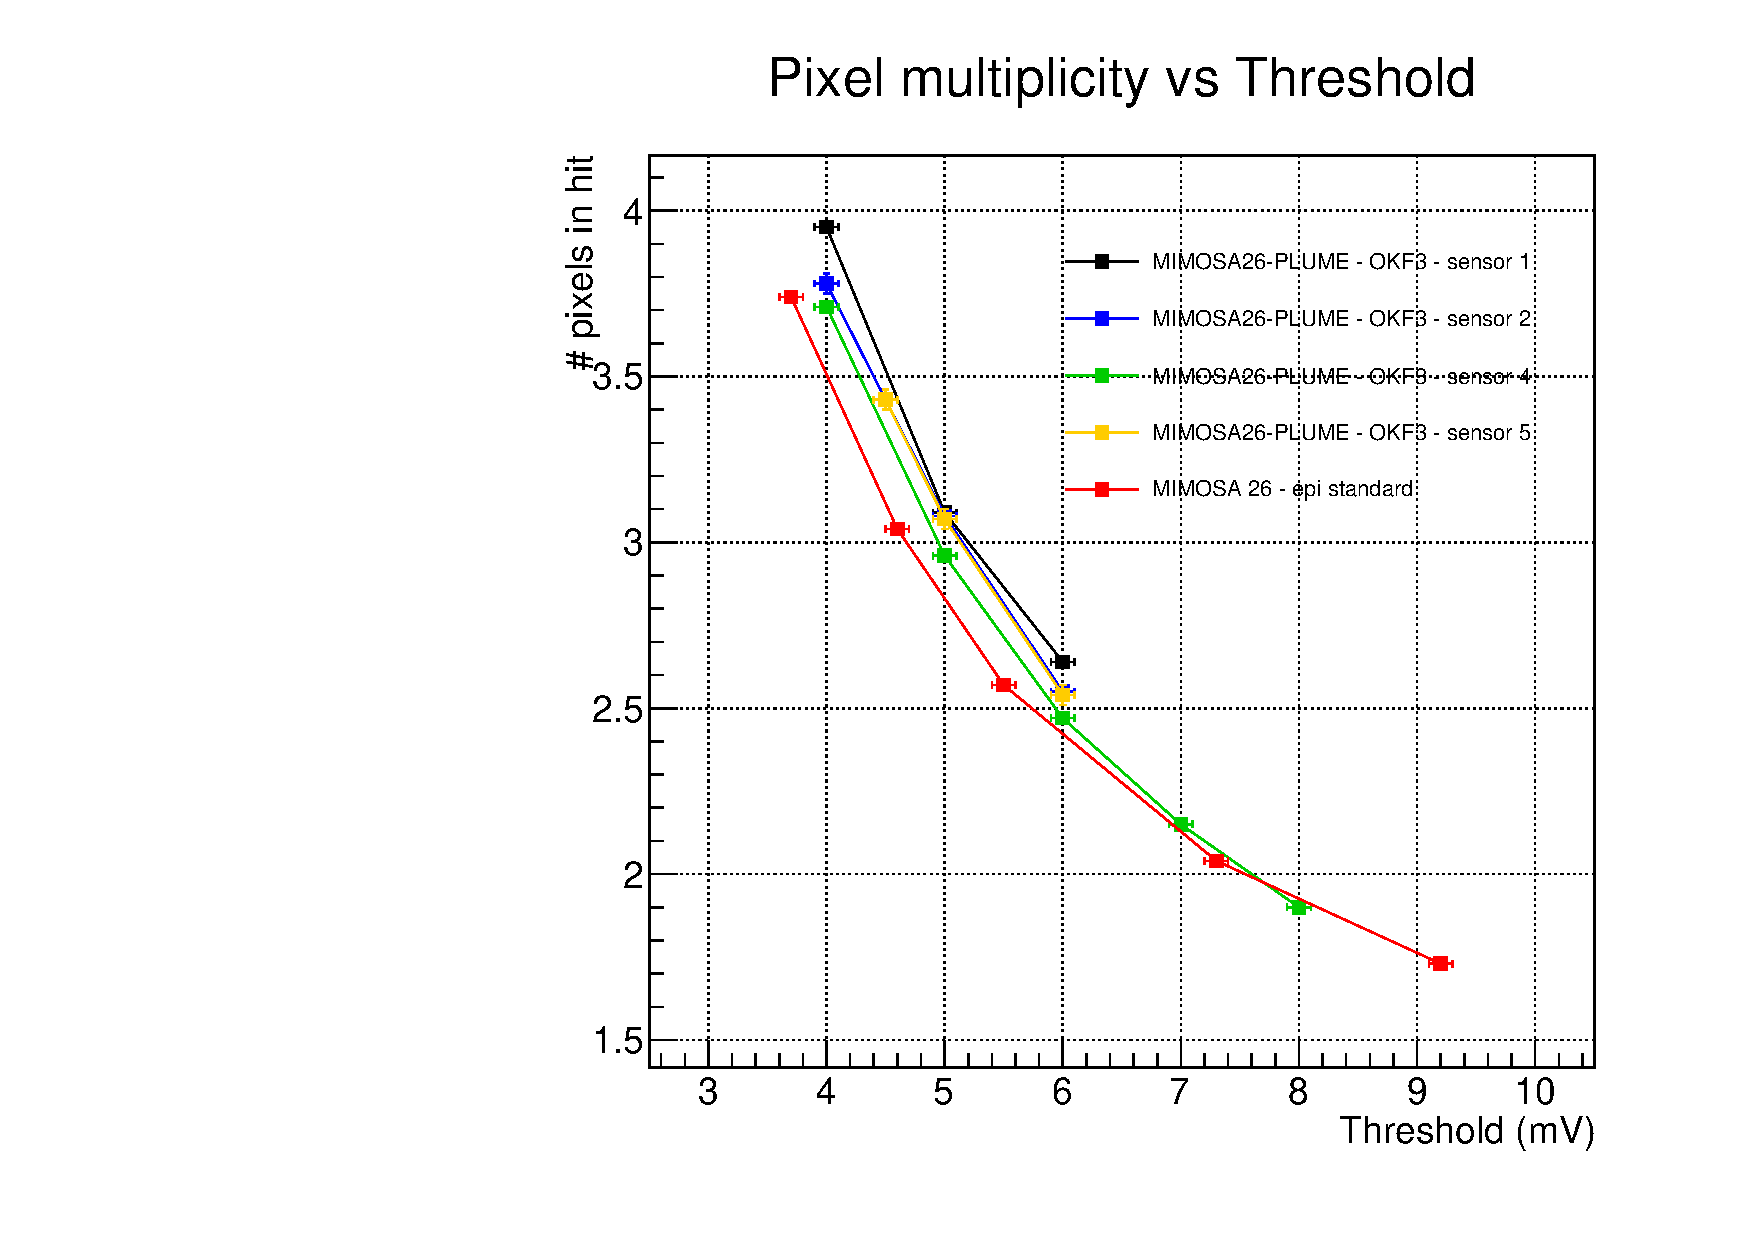
\includegraphics[scale=0.70]{./figures/Plots_PLUME/OKF3_Mult_Thr_mV.pdf}
%     \caption{Multiplicit\'es des amas pour les capteurs 1, 2, 4 et 5 de la face OKF3 de l'\'echelle PLUME en fonction du seuil des discriminateurs en $mV$, compar\'ees avec la multiplicit\'e du capteur de r\'ef\'erence MIMOSA26 \'epi standard (en rouge).}
%     \label{fig:OKF3_mult}
%    \end{center}
%    \end{figure}
%    
%    La figure \ref{fig:OKF3_eff} rapporte l'efficacit\'e de d\'etection des capteurs mont\'es sur la face OKF3 en fonction de leur seuil de discriminateurs exprim\'e en $mV$. Les efficacit\'es obtenues sont compar\'es au capteur de r\'ef\'erence MIMOSA26 epi standard. Les efficacit\'e obtenues sont similaires et sont comparables au capteur de r\'ef\'erence.
   
%    \begin{figure}[!htb]
%    \begin{center} 
%     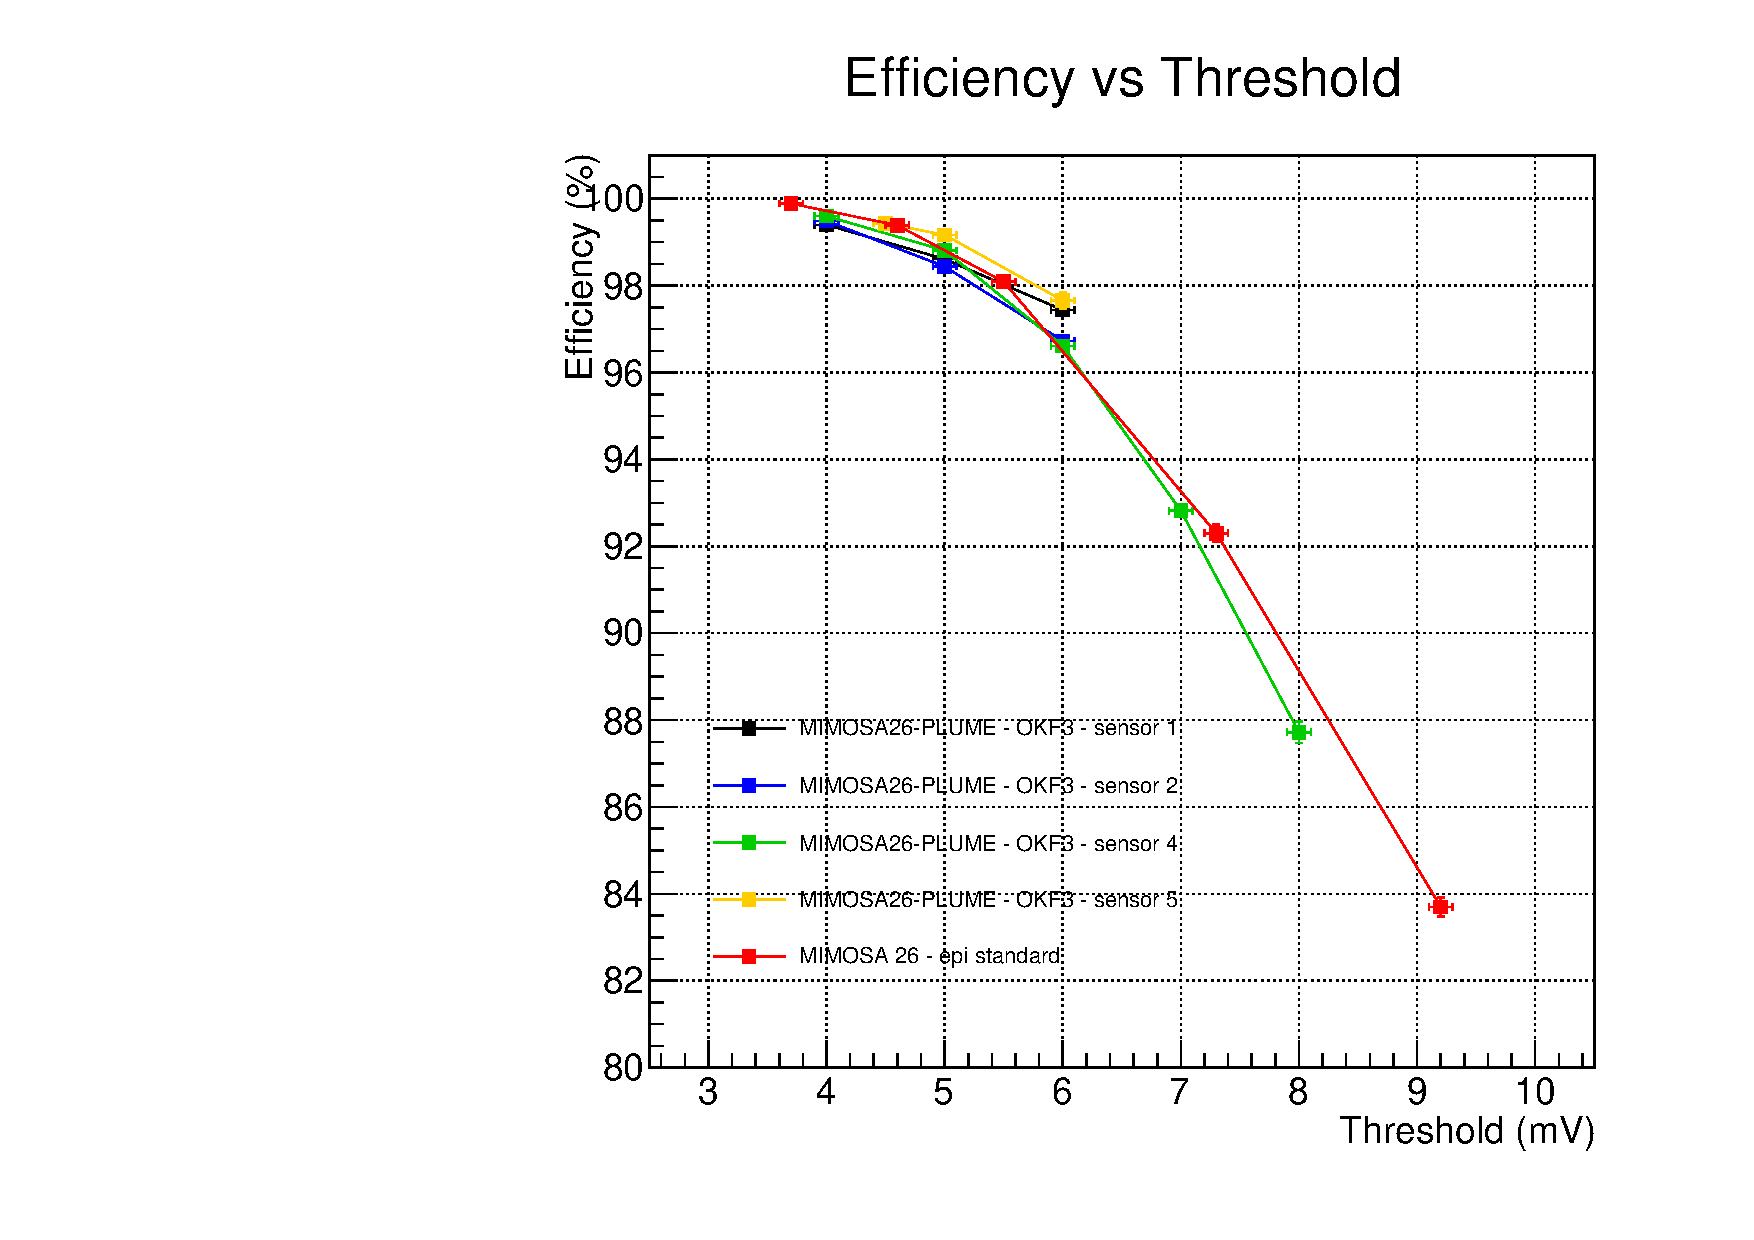
\includegraphics[scale=0.70]{./figures/Plots_PLUME/OKF3_Eff_Thr_mV.pdf}
%     \caption{Efficacit\'e de d\'etection des capteurs de la face OKF3 en fonction du seuil des discriminateurs en mV.}
%     \label{fig:OKF3_eff}
%    \end{center}
%    \end{figure}
   
%    La figure \ref{fig:OKF3_fake} r\'esume les performances en terme de taux d'impacts fant\^omes. Pour r\'ealiser ces mesures le faisceau a \'et\'e \'eteint et les donn\'ees ont \'et\'e enregistr\'ees pour diff\'erents seuil des discriminateurs en $mV$ de chaque capteur de la face OKF3. Les taux d'impacts fant\^omes ainsi obtenus pour les capteurs 1, 2, et 5 sont similaires au capteur de r\'ef\'erence. Pour ces capteurs la taux d'impacts fant\^omes est inf\'erieur ou \'egal \`a $10^{-4}$. Pour le capteur 4, le taux d'impacts fant\^omes mesur\'e est inf\'erieur de presque un ordre de grandeur.///// ............ Pourquoi ? variation du taux de fantomes selon le capteur ? -> variabilit\'e fabrication ? ................///
   
%    \begin{figure}[!htb]
%    \begin{center} 
%     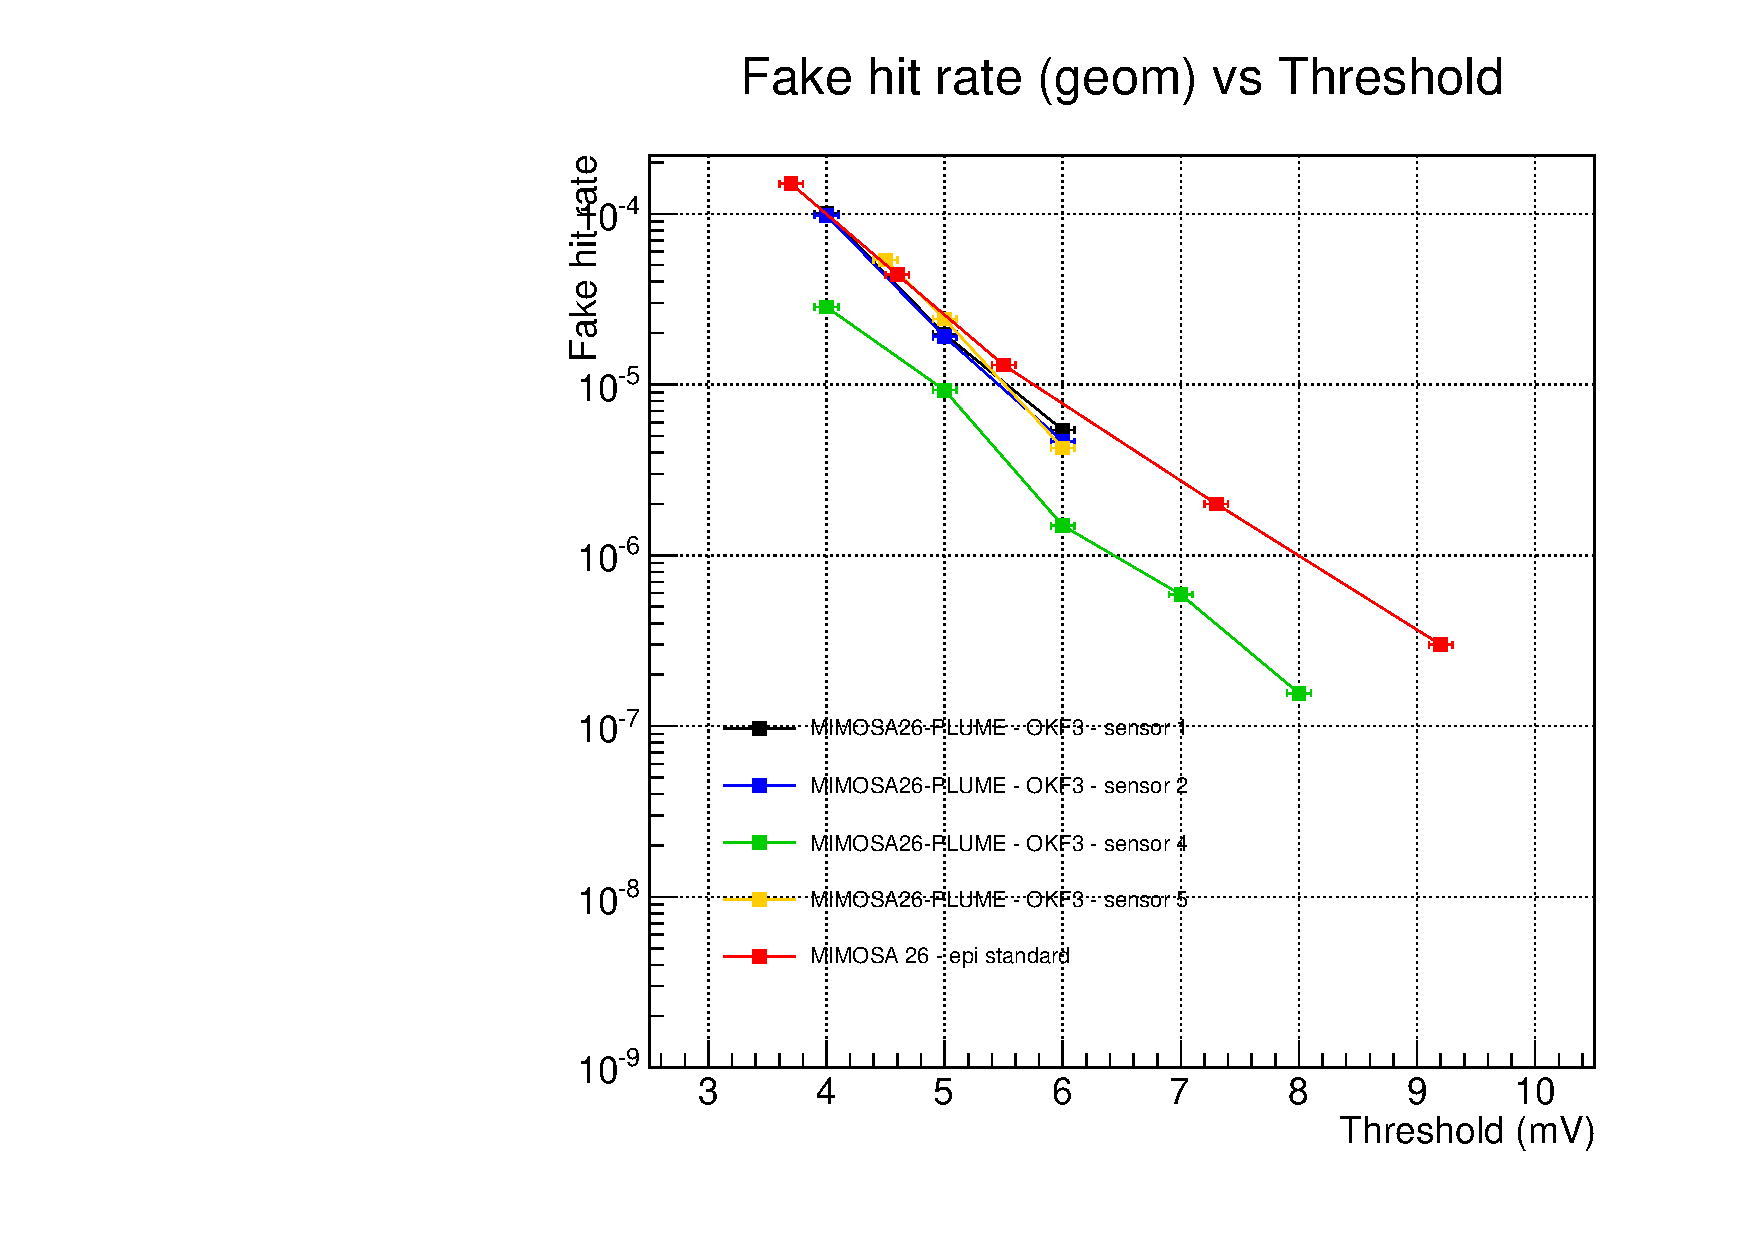
\includegraphics[scale=0.70]{./figures/Plots_PLUME/OKF3_Fake_Thr_mV.pdf}
%     \caption{Taux d'impacts fant\^omes des capteurs de la face OKF3 en fonction du seuil des discriminateurs en mV.}
%     \label{fig:OKF3_fake}
%    \end{center}
%    \end{figure}
    
%    La figure \ref{fig:OKF3_res} repr\'esente la r\'esolution spatiale des capteurs de la face OKF3 en fonction du seuil des discriminateurs en mV.
%    Cette r\'esolution est compar\'ee \`a celle du capteur de r\'ef\'erence MIMOSA26 epi standard. Aux erreurs pr\`es, pour cahque capteur de la face OKF3, la r\'esolution spatiale est comparable \`a celle du capteur de r\'ef\'erence.
   
%    \begin{figure}[!htb]
%    \begin{center} 
%     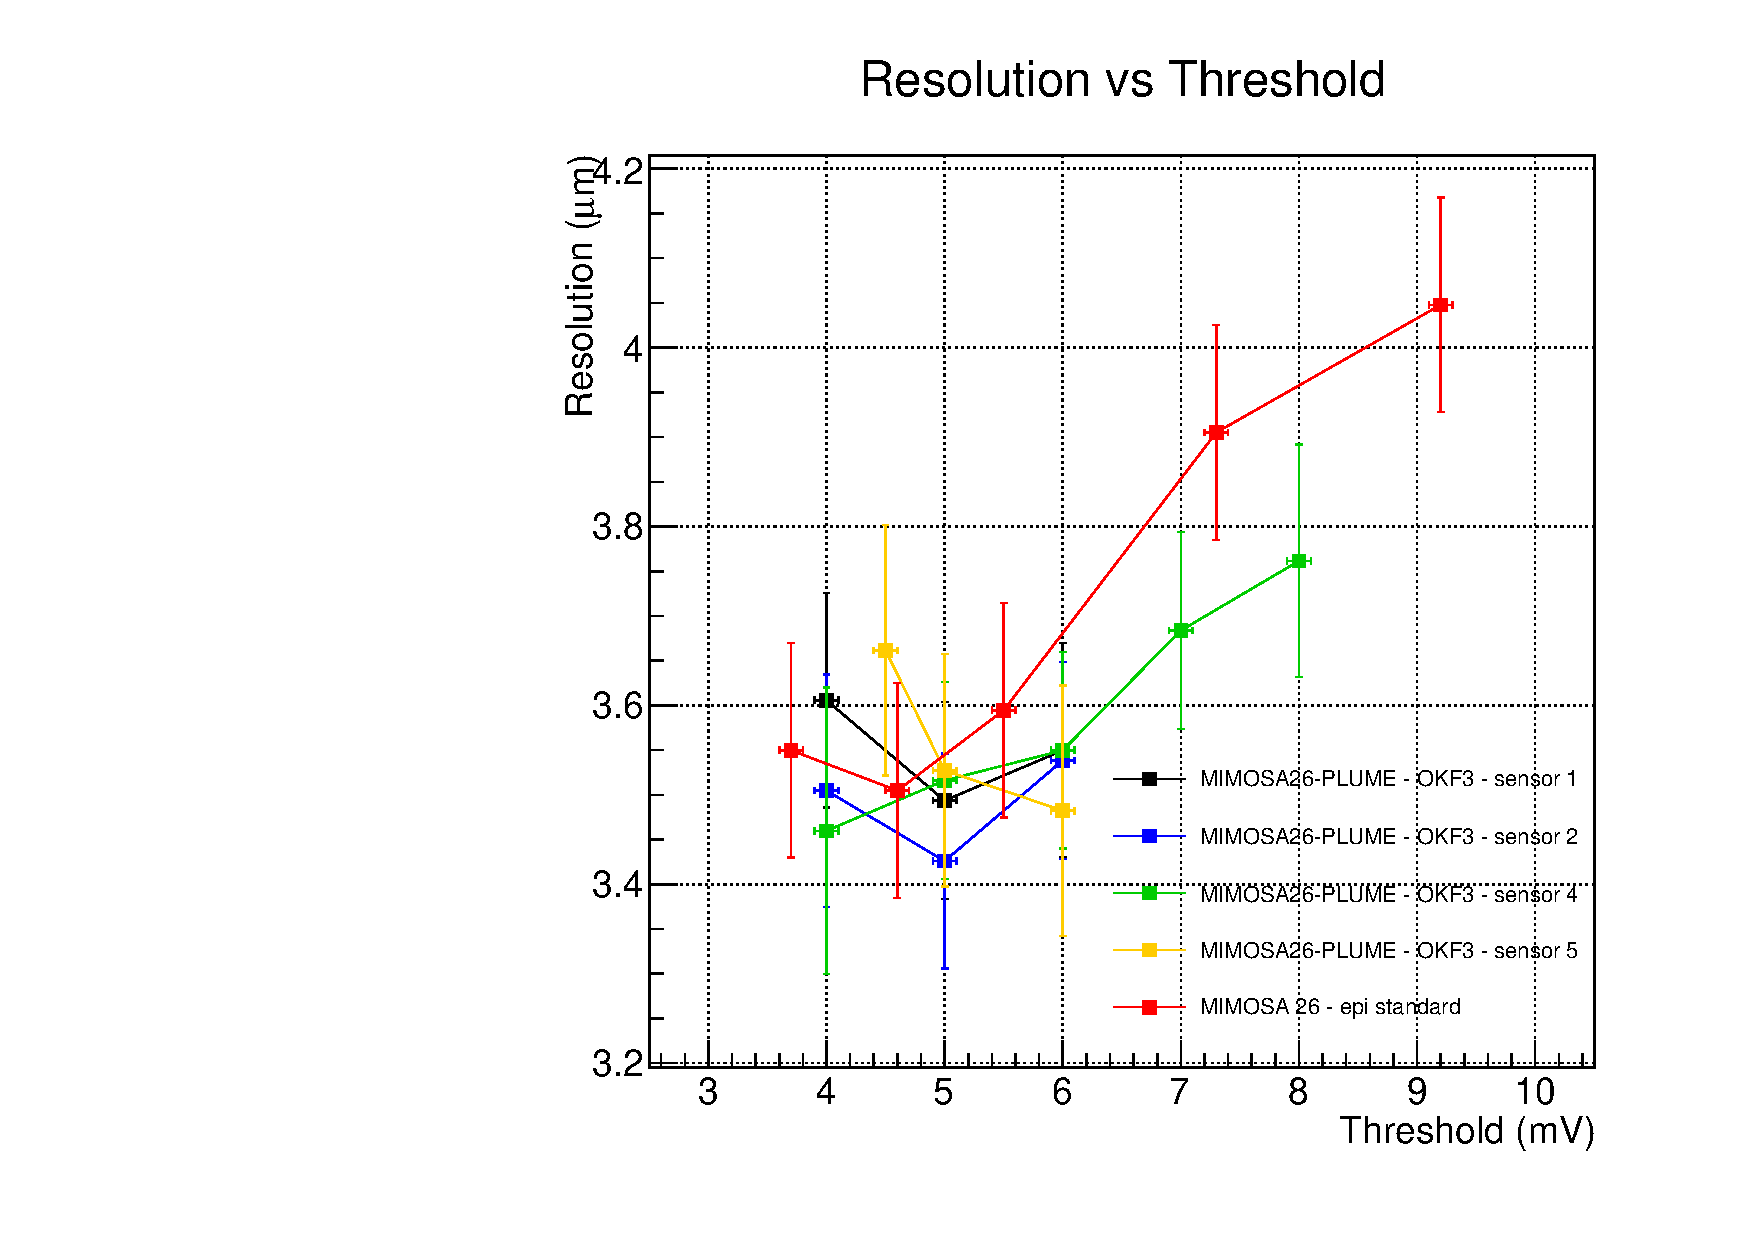
\includegraphics[scale=0.70]{./figures/Plots_PLUME/OKF3_Res_Thr_mV.pdf}
%     \caption{R\'esolution spatiale des capteurs de la face OKF3 en fonction du seuil des discriminateurs en mV.}
%     \label{fig:OKF3_res}
%    \end{center}
%    \end{figure}

%    \medskip
%    
%    Nous allons \`a pr\'esent \'etudier les caract\'eristiques des capteurs de la seconde face, OKF6, de l'echelle PLUME. De difficult\'ees suppl\'ementaires sont apparus lors de l'analyse des capteurs de cette face. Notament lors de la phase d'alignment................................................................................................................................................ 
% 
%    \medskip
%    DIRE LES PROBLEMES RENCONTReS ....
%    
%    
%    \medskip
%    
%    La figure \ref{fig:OKF6_mult} repr\'esente pour chaque capteur de la face OKF6, la multiplicit\'e des amas reconstruites en fonction du seuil en $mV$ appliqu\'e au discriminateurs de chaque capteur. L'\'ecart observ\'e entre le capteur de r\'ef\'erence et les capteurs de la face OKF6 est sup\'erieur \`a celui observ\'e entre le capteur de r\'ef\'erence et ceux la face OKF3. La multiplicit\'e est environ 5 $\%$ sup\'erieure pour le capteur 2 et reste environ 20 $\%$ sup\'erieure pour les capteurs 4 et 5. Pour caque capteur, le gain de multiplicit\'e observ\'e reste similaire pour tout les seuils appliqu\'es.

%    \begin{figure}[!htb]
%    \begin{center} 
%     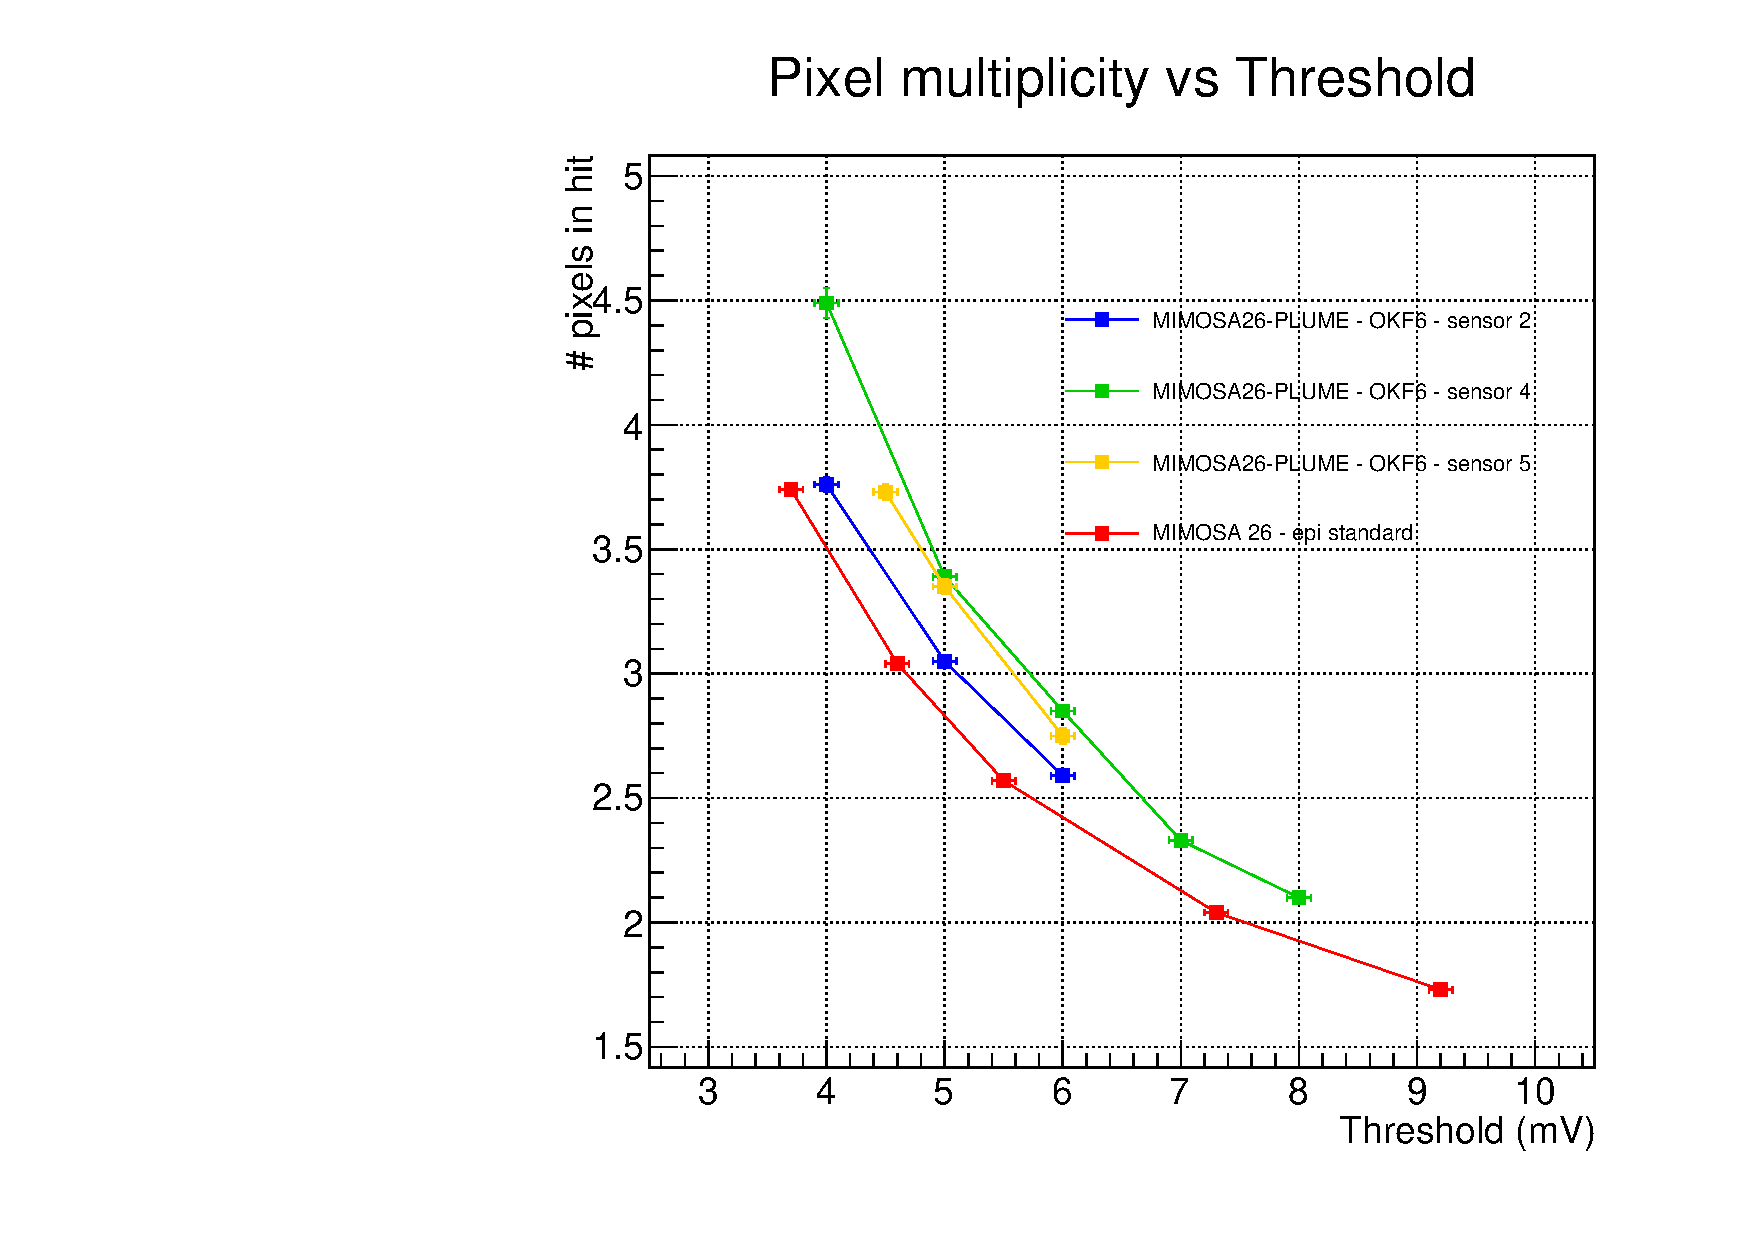
\includegraphics[scale=0.70]{./figures/Plots_PLUME/OKF6_Mult_Thr_mV.pdf}
%     \caption{Multiplicit\'e des amas des capteurs de la face OKF6 en fonction du seuil des discriminateurs en mV.}
%     \label{fig:OKF6_mult}
%    \end{center}
%    \end{figure}
   
%    La figure \ref{fig:OKF6_eff} repr\'esente l'efficacit\'e de d\'etection mesur\'e sur chaque capteur de la face OKF6 en fonction du seuil de discriminateur appliqu\'es. Cette fois-ci le capteur5 expose la m\^eme efficacit\'e que le capteur de r\'ef\'erence. Le capteur2 poss\`ede une efficacit\'e plus basse que le capteur de r\'ef\'erence entre les seuils de 4 \`a 6 $mV$. L'efficacit\'e de d\'etection pour le capteur 4 r\'egl\'e au seuil de 4 $mV$ est similaire \`a celle du capteur de r\'ef\'erence. Cependant, le capteur4 expose une efficacit\'e sup\'erieure au capteur de r\'ef\'erence pour un seuil des ces discriminateurs sup\'erieur \`a 4 $mV$.
%    
%    \medskip
%   
%    POURQUOI CES DIFFERENCES !!!???
%    
%    \medskip
%    
%    \begin{figure}[!htb]
%    \begin{center}
%     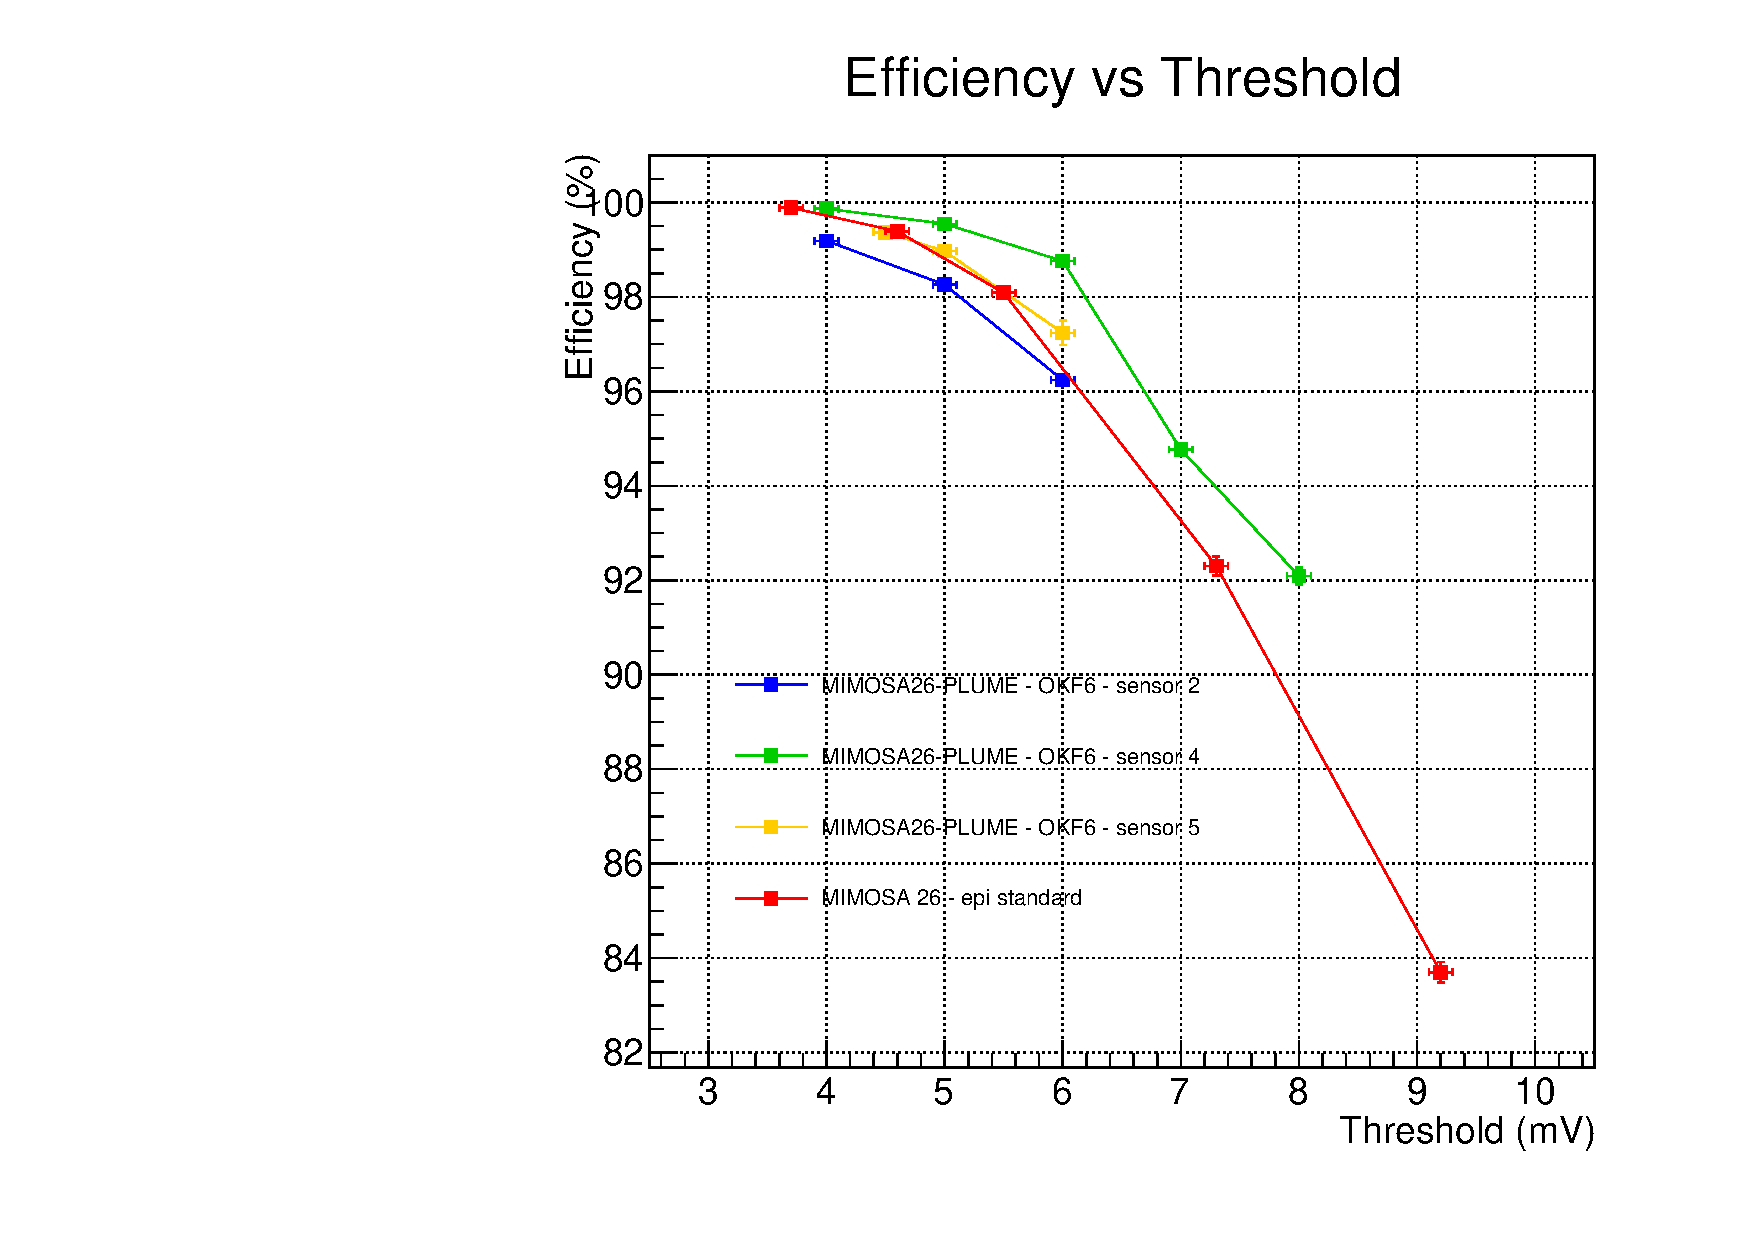
\includegraphics[scale=0.70]{./figures/Plots_PLUME/OKF6_Eff_Thr_mV.pdf}
%     \caption{Efficacit\'e de d\'etection des capteurs de la face OKF6 en fonction du seuil des discriminateurs en mV.}
%     \label{fig:OKF6_eff}
%    \end{center}
%    \end{figure}
   
%    La figure \ref{fig:OKF6_fake} repr\'esente le taux d'impacts fant\^ome pour les capteurs de la face OKF6 en fonction du seuil de leurs discriminateurs en $mV$. Pour obtenir ces r\'esultats le faisceau est coup\'e et le taux d'impacts fant\^omes est mesur\'e. Le taux de fant\^ome obtenu est identique \`a celui du capteur de r\'ef\'erence.
   
%    \begin{figure}[!htb]
%    \begin{center} 
%     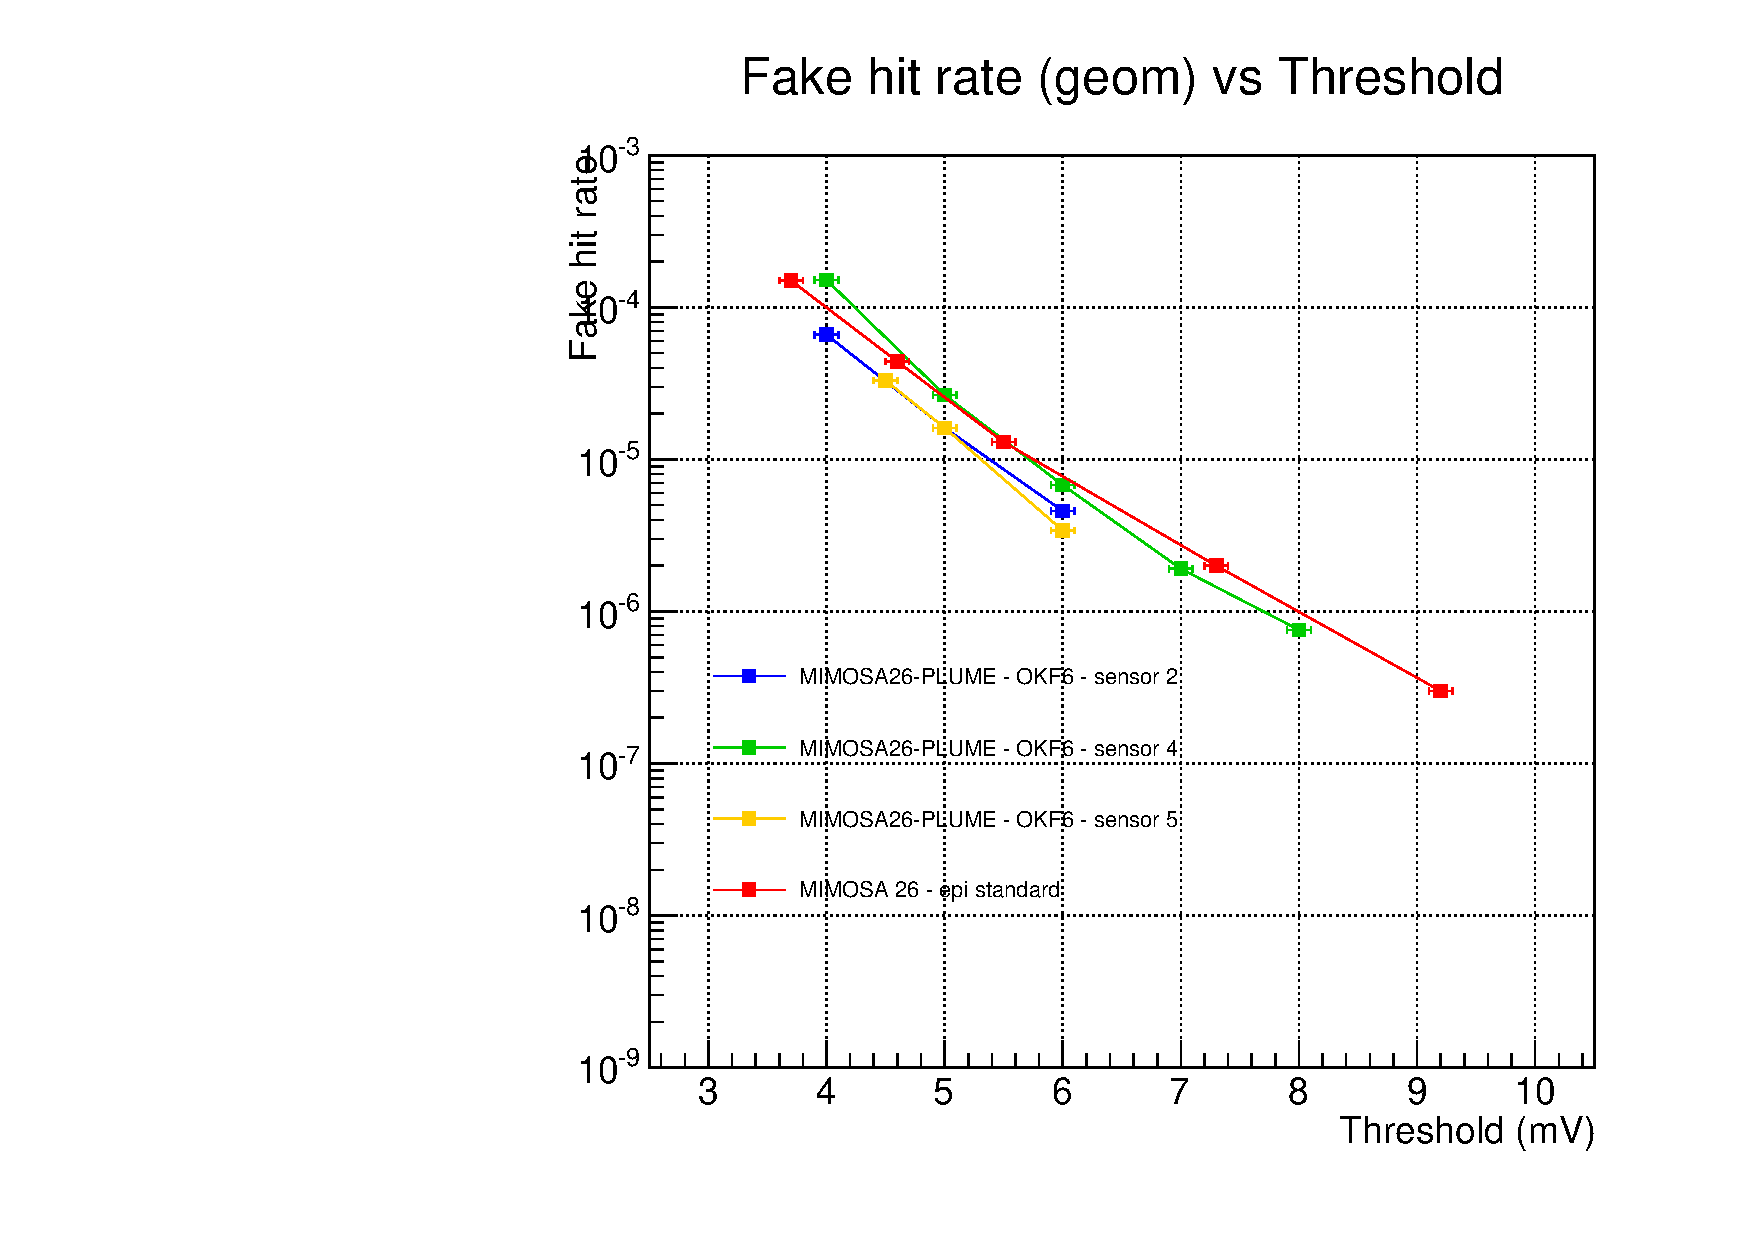
\includegraphics[scale=0.70]{./figures/Plots_PLUME/OKF6_Fake_Thr_mV.pdf}
%     \caption{Taux d'impacts fant\^omes des capteurs de la face OKF6 en fonction du seuil des discriminateurs en mV.}
%     \label{fig:OKF6_fake}
%    \end{center}
%    \end{figure}
    
%    La figure \ref{fig:OKF6_res} illustre la r\'esolution spatiale mesur\'ee pour chaque capteur de la face OKF6 de l'\'echelle PLUME test\'ee. Cette r\'esolution est mesur\'ee en fonction du seuil des discriminateurs de chaque capteur exprim\'es en $mV$. Compar\'e au capteur de référence et étant donn\'ee les incertitudes sur la mesure de chaque résolution spatiale, les r\'esolution obtenue pour les capteurs 2 et 5 sont compatibles avec celles du capteur de r\'ef\'erence. Cependant, les r\'esolutions spatiales obtenues pour le capteur 4 diff\`erent de celles du capteur de r\'ef\'erence pour un seuil de discriminateur r\'eglé aux valeurs de 7 et 8 $mV$. La r\'esolution alors obtenue est inf\'erieure d'environ 5 $\%$ par rapport \`a celle du capteur de r\'ef\'erence fonctionnant aux m\^emes seuils.
%     
%    \medskip
% 
%    POURQUOI CES DIFFERENCES CAR RESO INFERIEURE ET NON SUPERIEURE au capt de ref !!??
   
%    \begin{figure}[!htb]
%    \begin{center} 
%     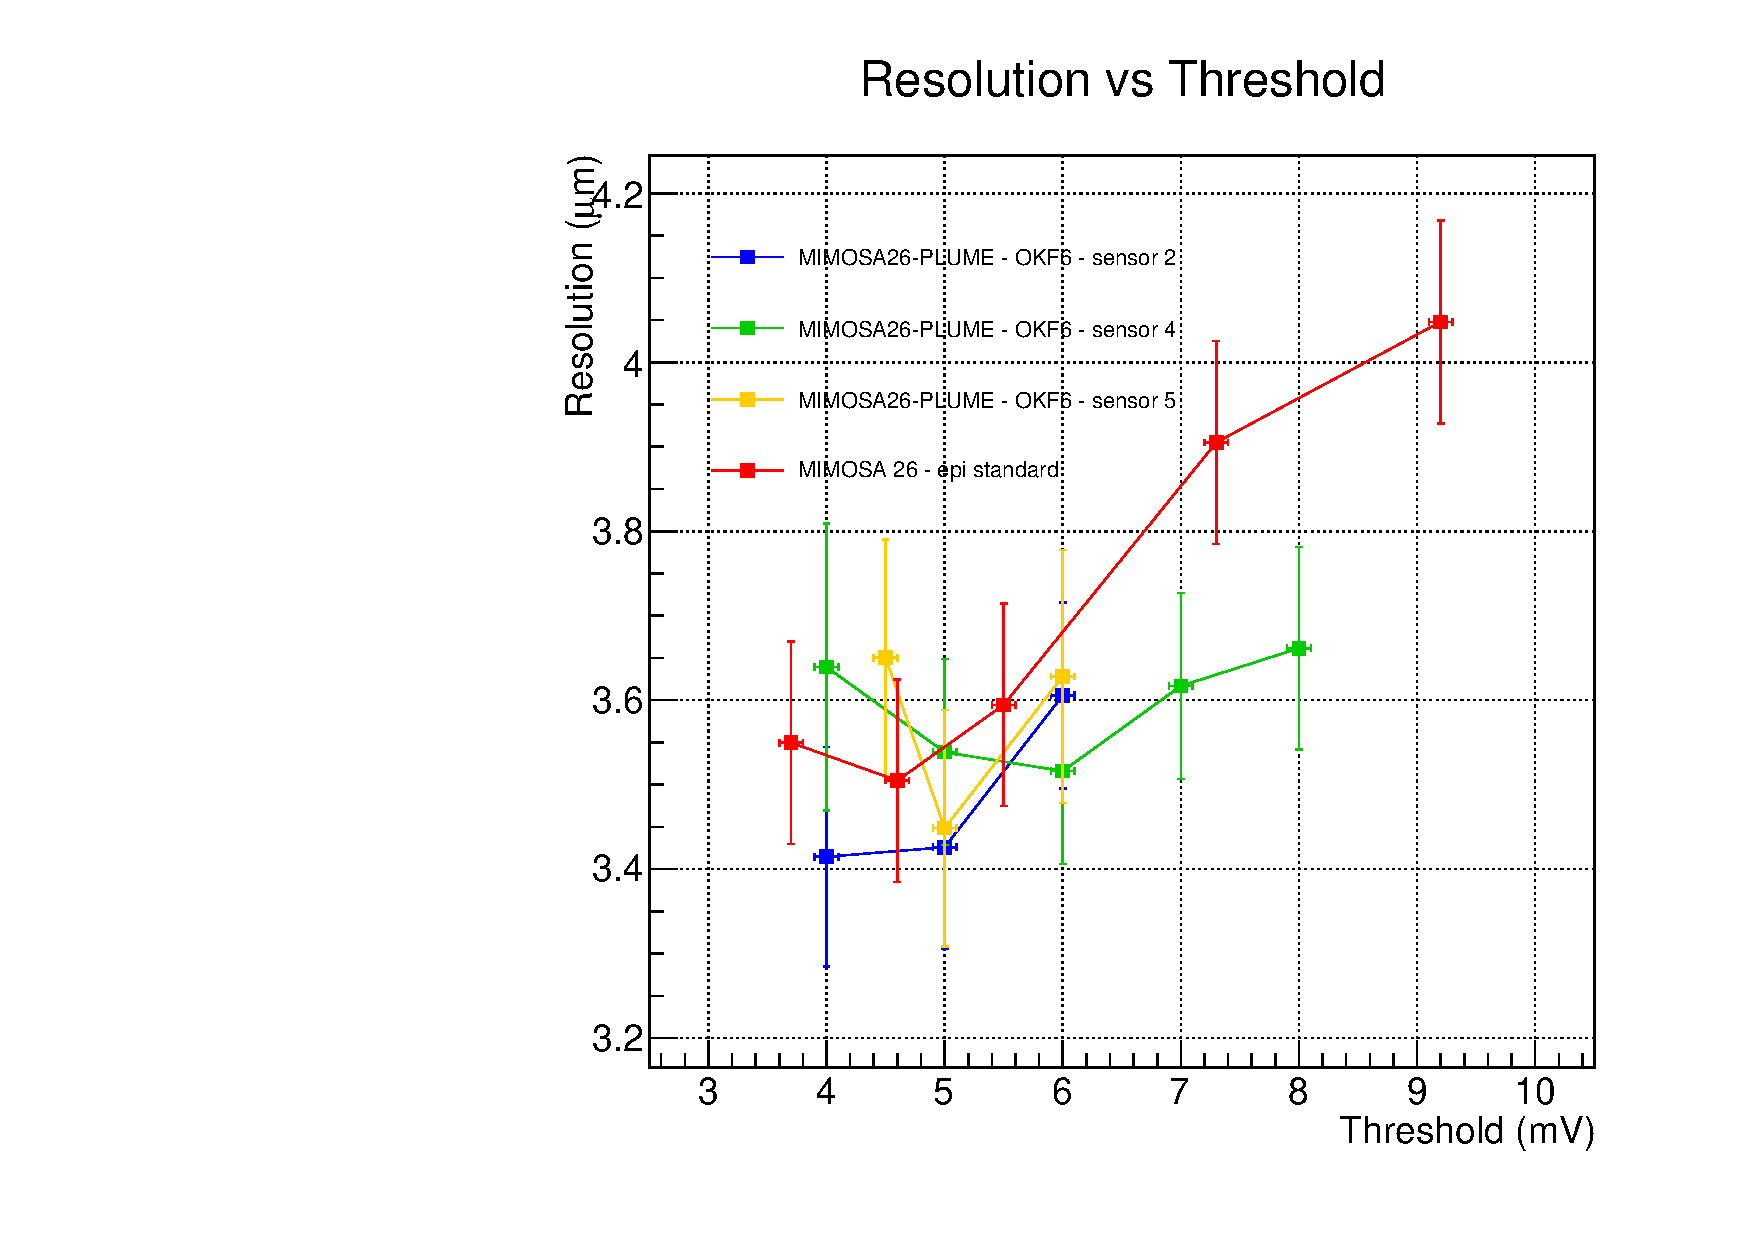
\includegraphics[scale=0.70]{./figures/Plots_PLUME/OKF6_Res_Thr_mV.pdf}
%     \caption{R\'esolution spatiale des capteurs de la face OKF6 en fonction du seuil des discriminateurs en mV.}
%     \label{fig:OKF6_res}   
%     \end{center}
%    \end{figure}
  
  \paragraph{Conclusion :}
  
   Nous avons explor\'e les diff\'erentes caract\'eristiques des 12 capteurs MIMOSA-26 constituant l'\'echelle PLUME. Nous voulions tester la bonne r\'eponse de ces capteurs sur l'\'echelle ainsi que l'homog\'en\'eit\'e de leurs caract\'eristiques cl\'ees. Nous avons vu que l'efficacit\'e de d\'etection, le taux d'impacts fant\^omes ainsi que la r\'esolution spatiale affichent des valeurs compatibles avec celles du capteur de r\'ef\'erence MIMOSA-26. Cependant, quelques disparit\'es avec le capteur de r\'ef\'erence ont \'et\'e identifi\'ees. Des \'ecarts d'environ 5 \`a 20 $\%$ en terme de multiplicit\'e moyenne des amas de pixels ont \'et\'e mesur\'es. Ces d\'eviations indiquent un signal plus fort compar\'e au capteur de r\'ef\'erence. Un signal plus \'elev\'e se traduit aussi par une augmentation de l'efficacit\'e de d\'etection. Cependant \'etant donn\'e les valeurs importantes de l'efficacit\'e \`a bas seuil, cet effet est moins visible sur les courbes d'efficacit\'e. Cette augmentation de signal dans les pixels peut \^etre expliqu\'ee par le calibrage des capteurs. Cela expliquerait aussi les disparit\'es obtenues en fonction du capteur test\'e.
   
   \medskip

   Au vu des r\'esultats obtenus, on peut conclure que les perturbations inter-capteurs sont faibles voir inexistantes. L'assemblage des capteurs sur un m\^eme support faisait craindre des perturbations thermiques ou \'electro-magn\'etiques. Cela n'a pas \'et\'e observ\'e, puisque le taux d'impacts fant\^omes et l'efficacit\'e de d\'etection restent quasiment inchang\'es compar\'es au capteur de r\'ef\'erence MIMOSA-26. Le refroidissement passif de l'\'echelle est donc valid\'e. De plus, la r\'esolution spatiale observ\'ee ne varie que tr\`es peu et est compatible aux erreurs pr\`es au capteur de r\'ef\'erence. Cette affirmation reste toutefois \`a prouver lors de l'inclinaison de l'\'echelle.
   
  \subsubsection{Inclinaison de l'échelle}
  
  Des donn\'ees en incidence non-normales avec l'\'echelle PLUME ont \'et\'e prises lors du test en faisceau de 2011. L'\'echelle PLUME a ainsi \'et\'e inclin\'ee d'environ 30, 36 et 40 degr\'es par rapport \`a l'axe vertical $V$ des capteurs \'etudi\'es. La configuration du t\'elescope reste la m\^eme que pr\'ec\'edemment pour ces inclinaisons. D'autres donn\'ees ont \'et\'e enregistr\'ees avec une inclinaison de l'\'echelle d'environ 60 degr\'es. Pour des raisons d'encombrement, l'\'echelle PLUME inclin\'ee \`a 60 degr\'es a du \^etre plac\'ee en aval du t\'elescope. Le t\'elescope a alors \'et\'e configur\'e diff\'eremment.
  
  \medskip
  
  La nouvelle configuration du t\'elescope pour l'\'echelle PLUME inclin\'ee \`a 60 degr\'es est montr\'ee en figure \ref{fig:tel_60deg}. Selon l'axe du faisceau que nous appellerons axe $Oz$, l'\'echelle PLUME croise le faisceau en premier, puis elle est suivie des 4 capteurs MIMOSA-26 r\'egl\'es avec un seuil de 8 fois leur bruit moyen. Selon cet axe $Oz$, le centre $O$ du t\'elescope est d\'efini par le centre du module compos\'e des deux premiers capteurs. Dans ce module, le capteur 1 croisant le faisceau en premier est plac\'e \`a $-5 \, mm$ du centre $O$ et le capteur 2 \`a $+5 \, mm$. Le second module de 2 capteurs est plac\'e \`a $+45 \, mm$ du centre $O$. Les capteurs 3 et 4 sont ainsi respectivement situ\'es \`a $40$ et $50 \, mm$ du point $O$. Le centre de l'\'echelle PLUME est quant \`a lui positionn\'e \`a $-120 \, mm$ du centre O selon l'axe $0z$. 

   \begin{figure}[!htb]
   \begin{center} 
    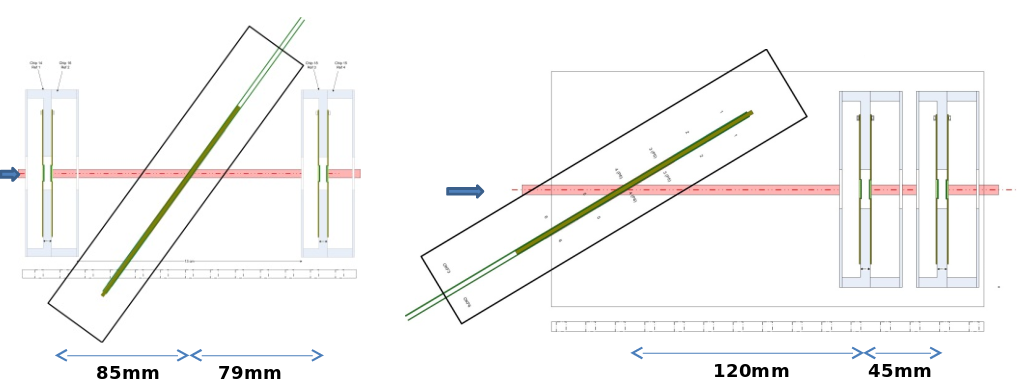
\includegraphics[scale=0.38]{./figures/PLULE_tilt_CONFIGs.png}
    \caption{Illustration des deux configurations du t\'elescope pour l'\'echelle PLUME inclin\'ee. \`A gauche : configuration pour des angles inf\'erieurs \`a 60 degr\'es. \`A droite configuration pour l'\'echelle PLUME inclin\'ee \`a 60 degr\'es.}
    \label{fig:tel_60deg}   
    \end{center}
   \end{figure}
  
  \medskip
  
  Les diff\'erentes prises de donn\'ees aux diff\'erents angles ont \'et\'e align\'ees et l'analyse des caract\'eristiques des capteurs selon ces diff\'erents angles ont \'et\'e effectu\'ees. Cependant, faute de temps, les r\'esultats n'ont pas atteint une maturit\'e suffisante. Des analyses plus pouss\'ees ont \'et\'e conduites par la suite par \textit{Robert Maria}, doctorant dans le groupe \textit{PICSEL}.
  
  \medskip
   
%   \begin{figure}[!htb]
%    \begin{center} 
%     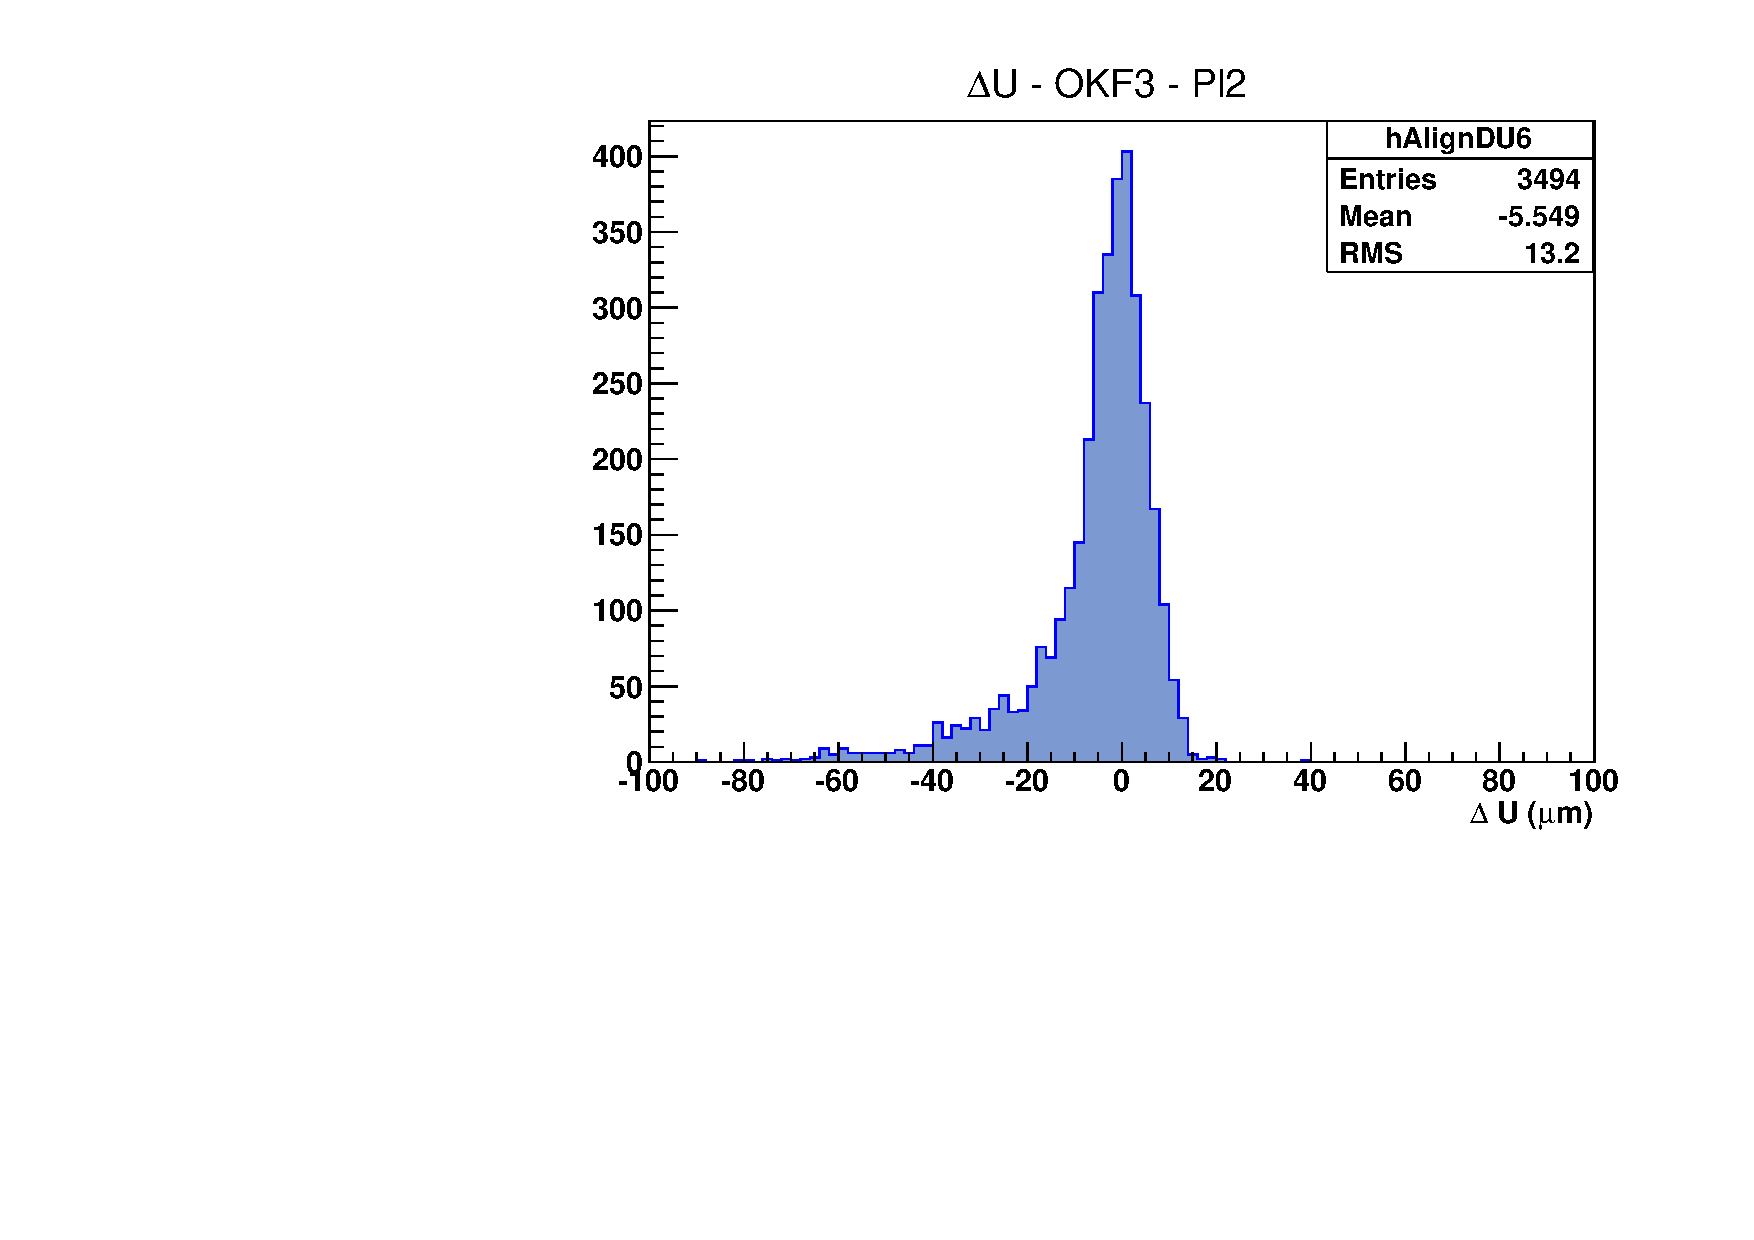
\includegraphics[scale=0.50]{./figures/PLUME_deformations/ResU_OKF3_Pl2.pdf}
%     \caption{Distribution des r\'esidus selon l'axe horizontal U.}
%     \label{fig:ResDefU}
%    \end{center}
%   \end{figure}
%   
%   \begin{figure}[!htb]
%    \begin{center} 
%     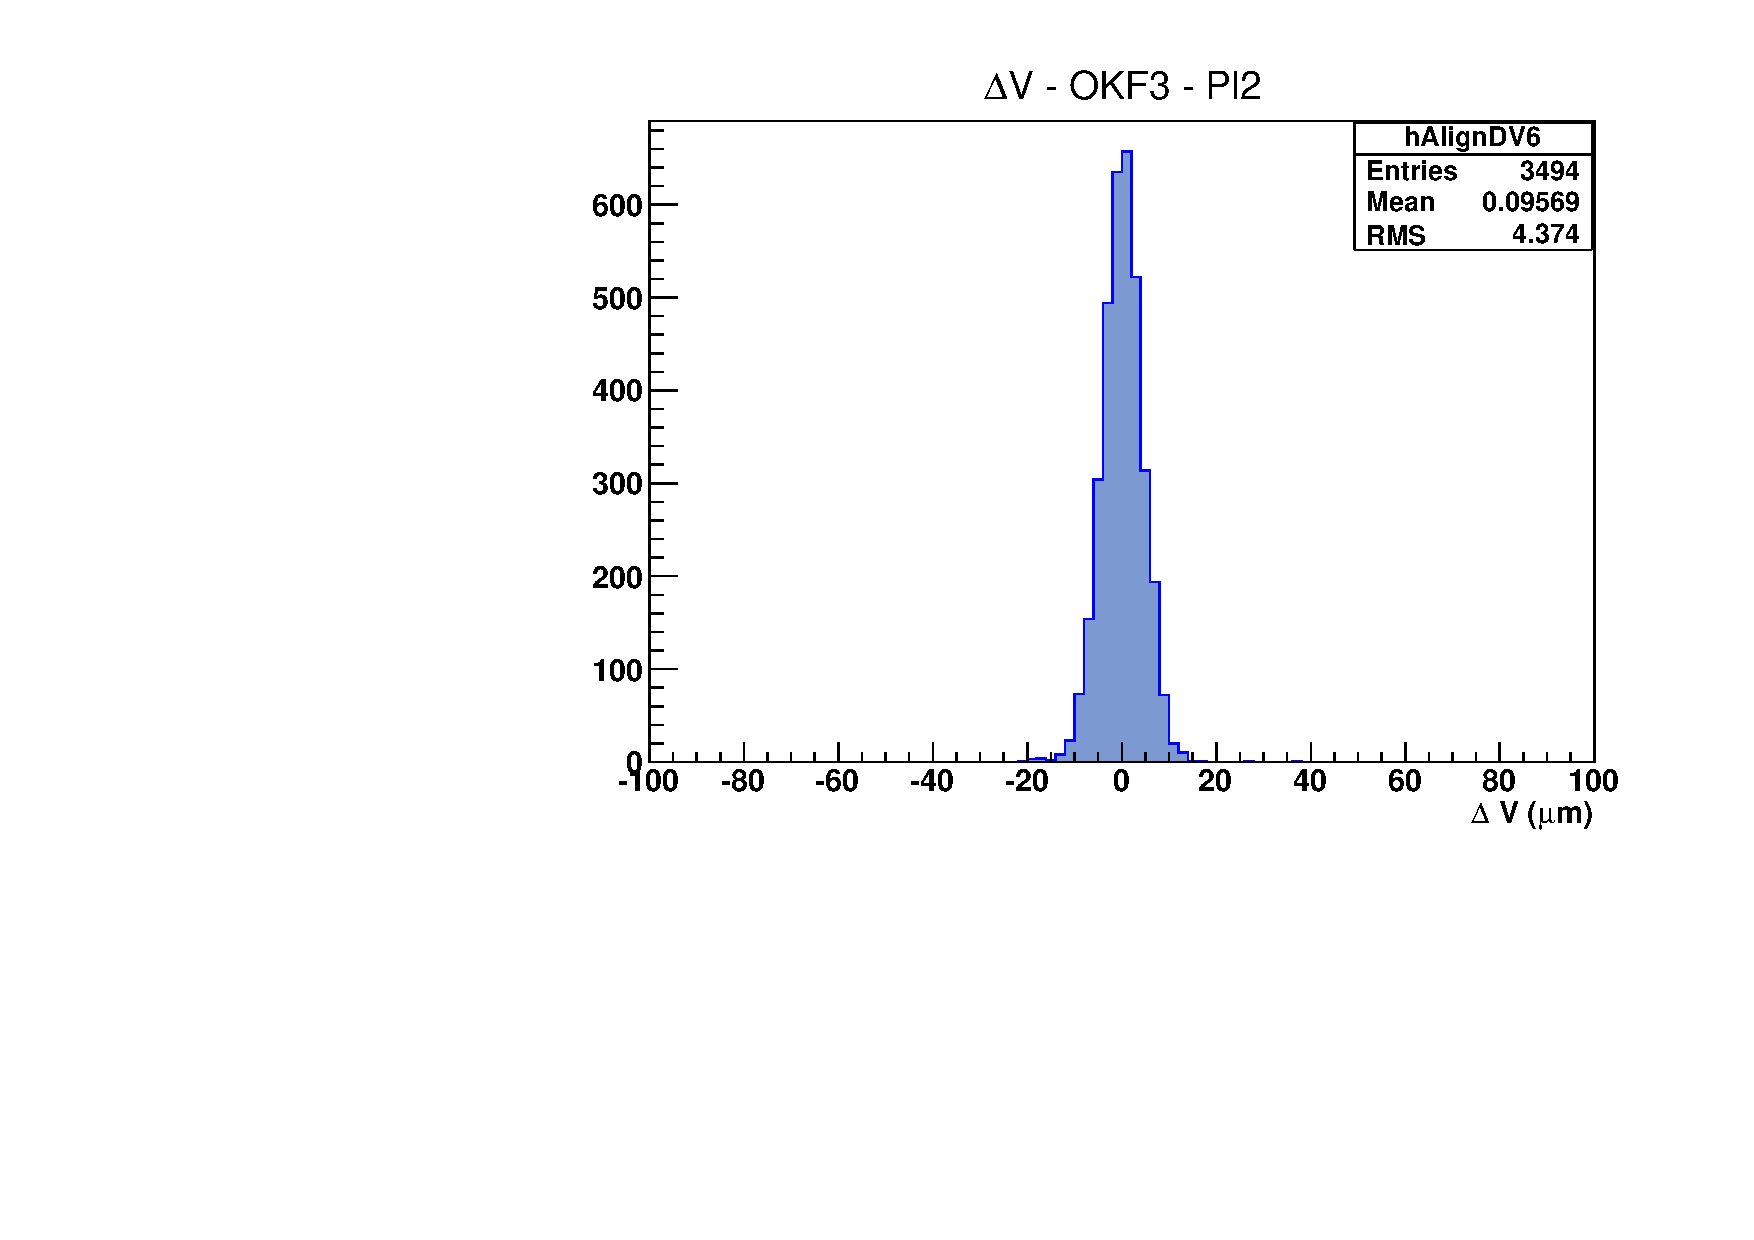
\includegraphics[scale=0.50]{./figures/PLUME_deformations/ResV_OKF3_Pl2.pdf}
%     \caption{Distribution des r\'esidus selon l'axe horizontal V.}
%     \label{fig:ResDefU}
%    \end{center}
%   \end{figure}
%   
  L'\'etude de l'alignement des capteurs de l'\'echelle PLUME inclin\'ee a permis, lors de cette th\`ese, de mettre en \'evidence des d\'eformations de la distribution des r\'esidus. Ces d\'eformations ont \'et\'e \'etudi\'ees par \textit{Robert Maria}. La suite de cette section se veut illustrative et d\'ecrit l'effet des d\'eformations des capteurs sur les r\'esidus. Les figures utilis\'ees dans la suite de cette section montrant les r\'esidus associ\'es aux d\'eformations des capteurs proviennent du travail de \textit{Robert Maria}.
  
  \medskip
  
  \begin{figure}[htb!]
     \begin{center}
        \subfigure[Distribution des r\'esidus selon l'axe horizontal U.]{
            \label{fig:ResU_Pl2_Tilted}
            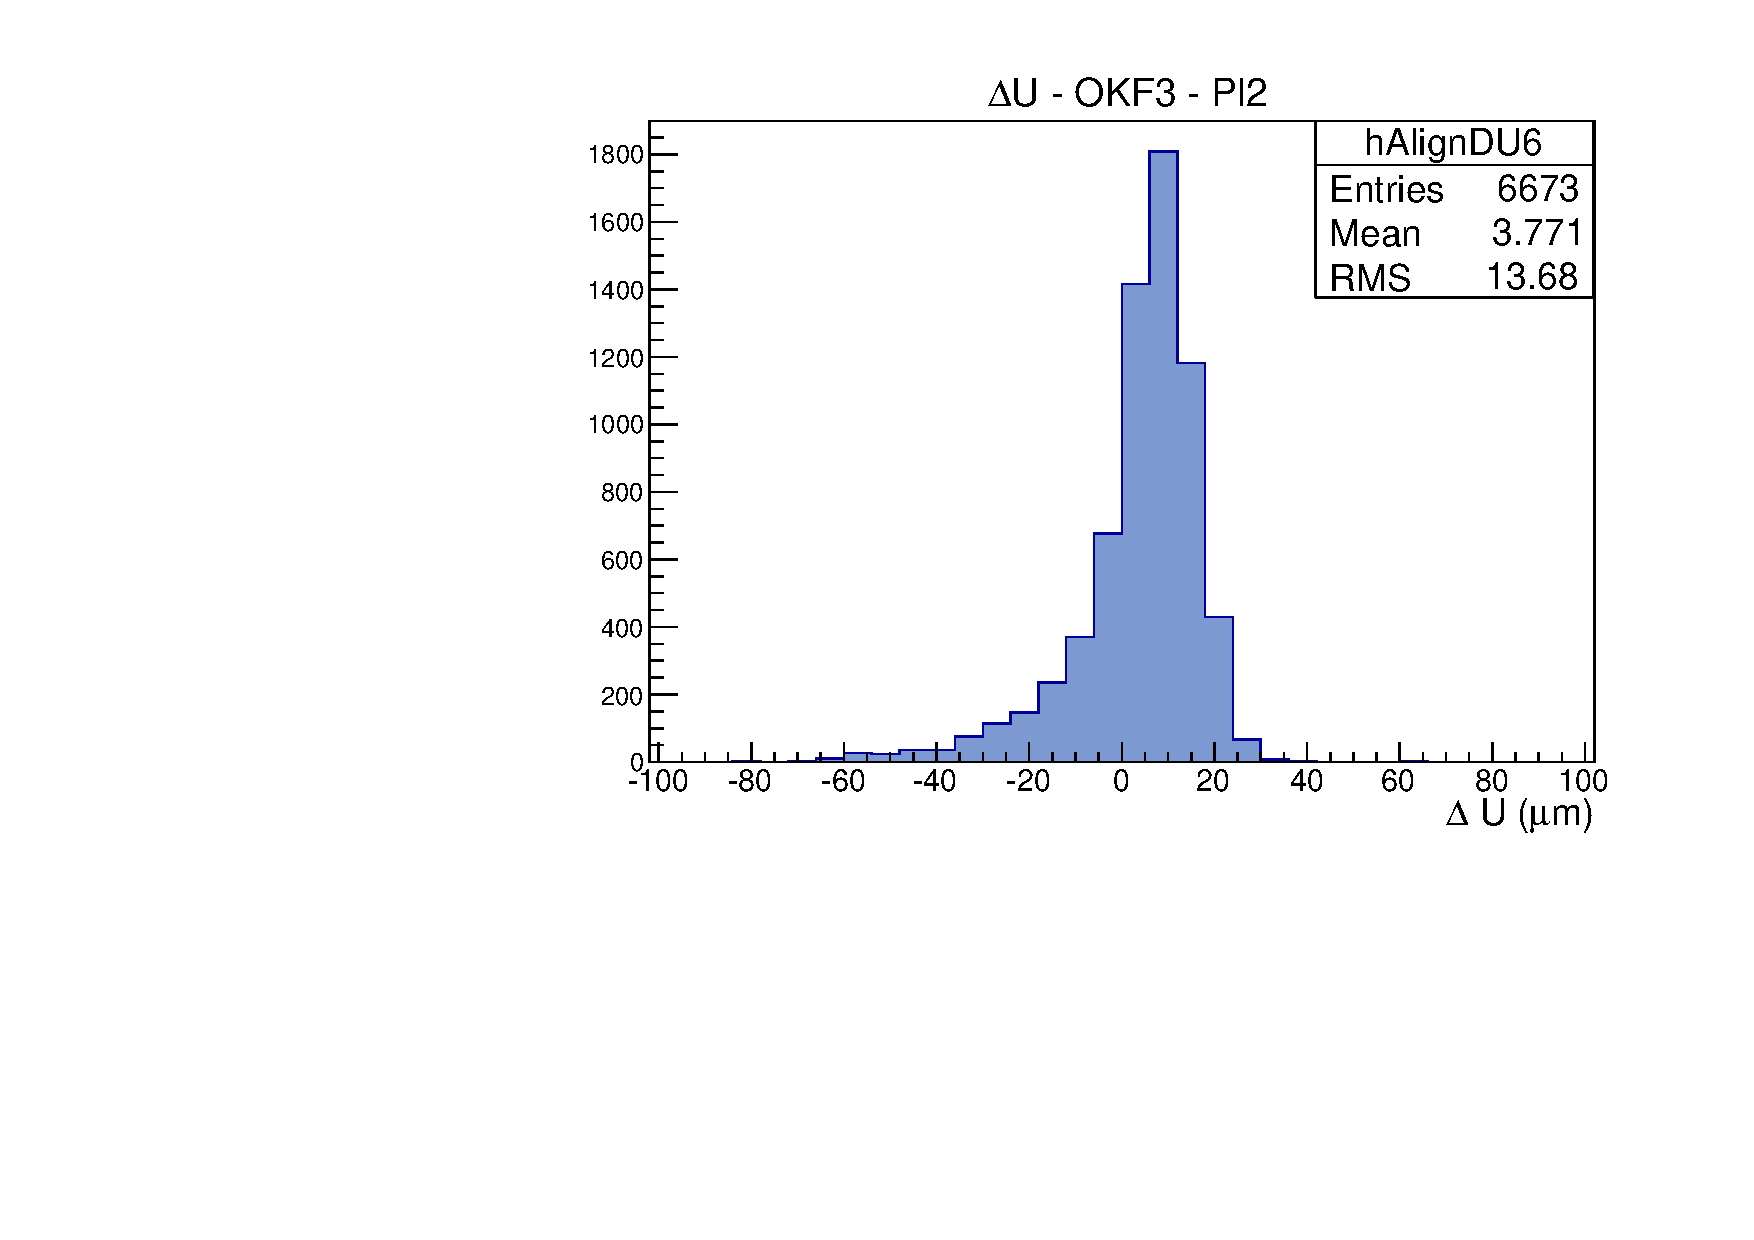
\includegraphics[width=0.45\textwidth]{./figures/PLUME_deformations/DeltaU_Pl2_OKF3_Loic.pdf}
        }
        \subfigure[Distribution des r\'esidus selon l'axe horizontal V.]{
            \label{fig:ResV_Pl2_Tilted}
            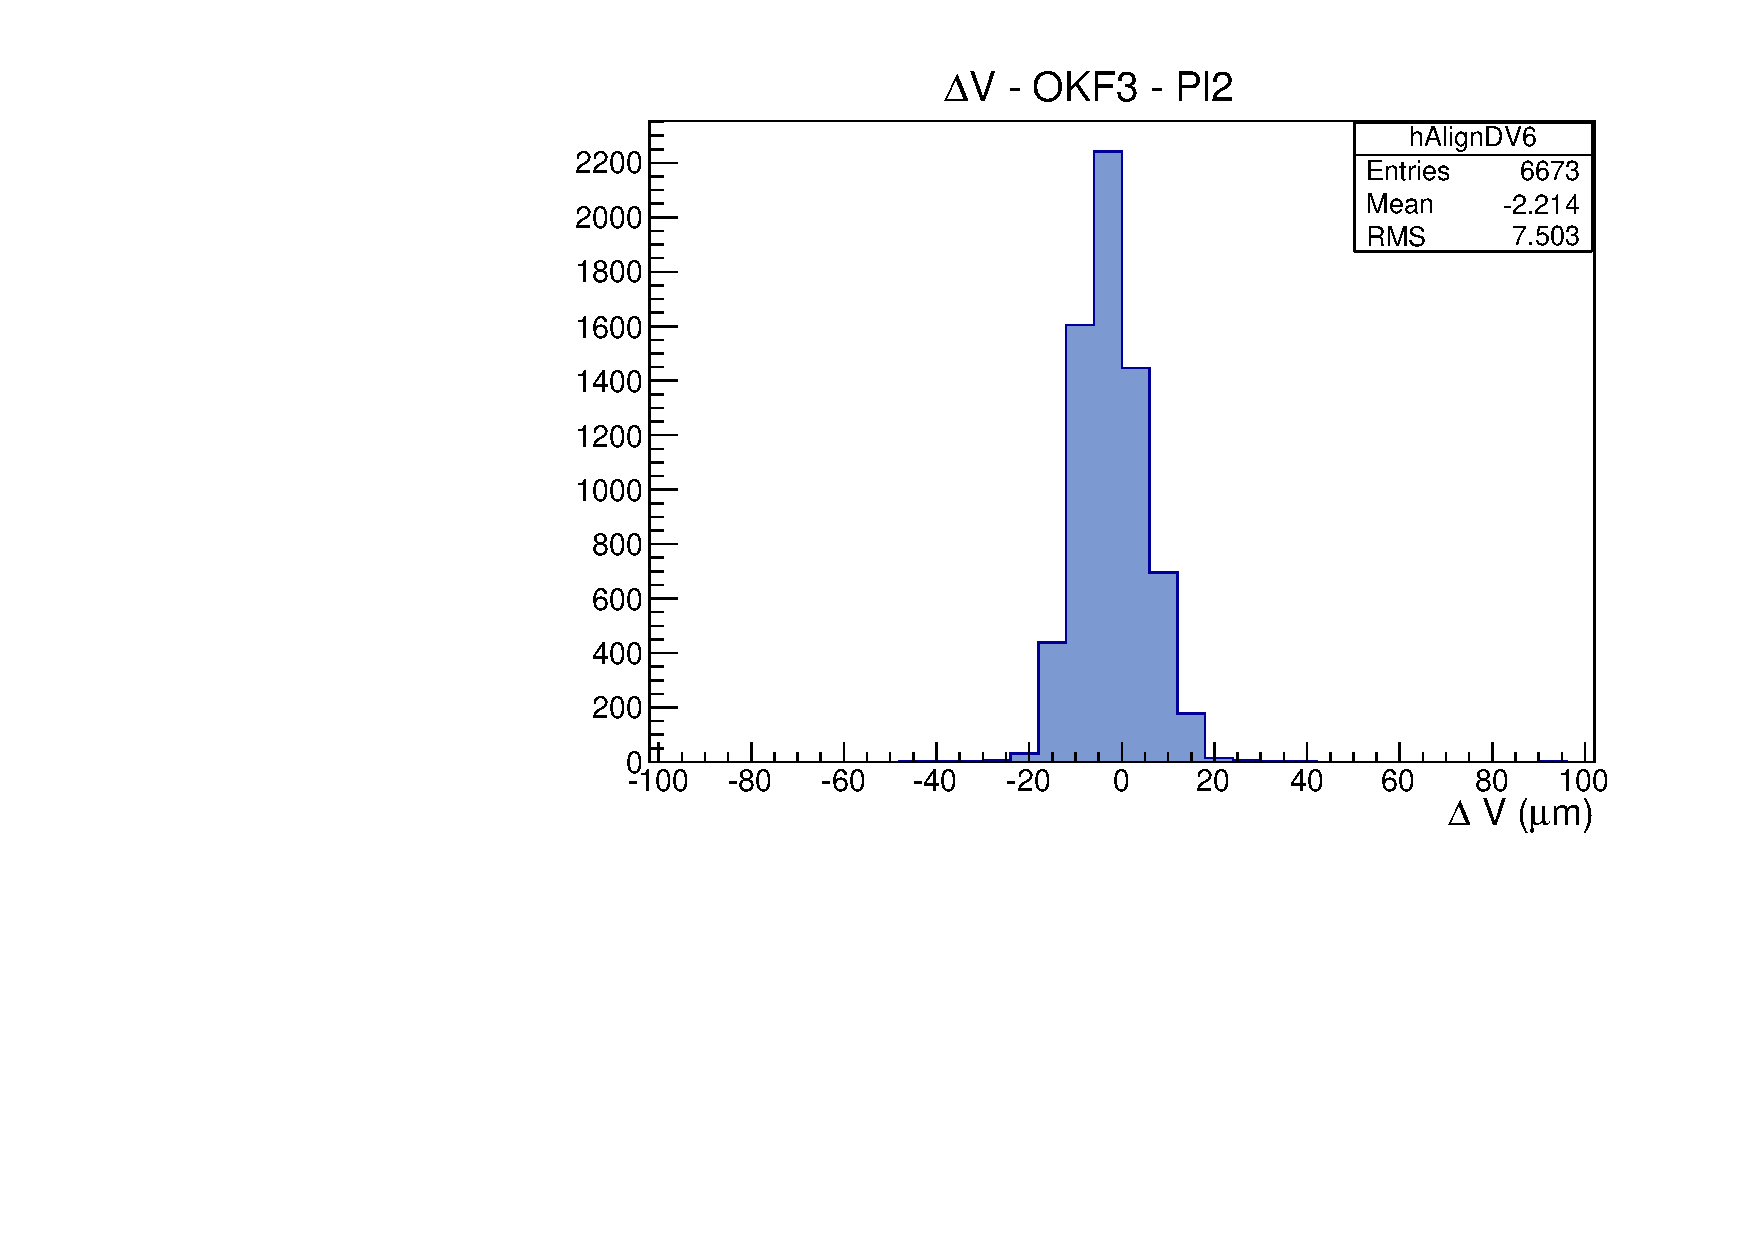
\includegraphics[width=0.45\textwidth]{./figures/PLUME_deformations/DeltaV_Pl2_OKF3_Loic.pdf}
        }
     \end{center}
     \caption{Distribution des r\'esidus pour le capteur 2 de la face \textit{OKF3} inclinée \`a 36 degr\'es.}
     \label{fig:Pl2Tilted}
  \end{figure}
  
  Lorsque l'\'echelle PLUME est inclin\'ee, la distribution des r\'esidus n'est plus Gaussienne. Les figures \ref{fig:ResU_Pl2_Tilted} et \ref{fig:ResV_Pl2_Tilted} illustrent les distributions des r\'esidus pour le capteur 2 de la face \textit{OKF3} inclin\'ee \`a 36 degr\'es. On observe que la distribution des r\'esidus selon l'axe horizontal $U$ du capteur n'est plus Gaussienne. La distribution poss\`ede des r\'esidus n\'egatifs plus grands que ceux que l'on obtiendrait avec une distribution Gaussienne. La distribution des r\'esidus par rapport \`a l'axe vertical $V$ reste quant \`a elle Gaussienne.
  
  \medskip
  
  \begin{figure}[!htb]
   \begin{center}
    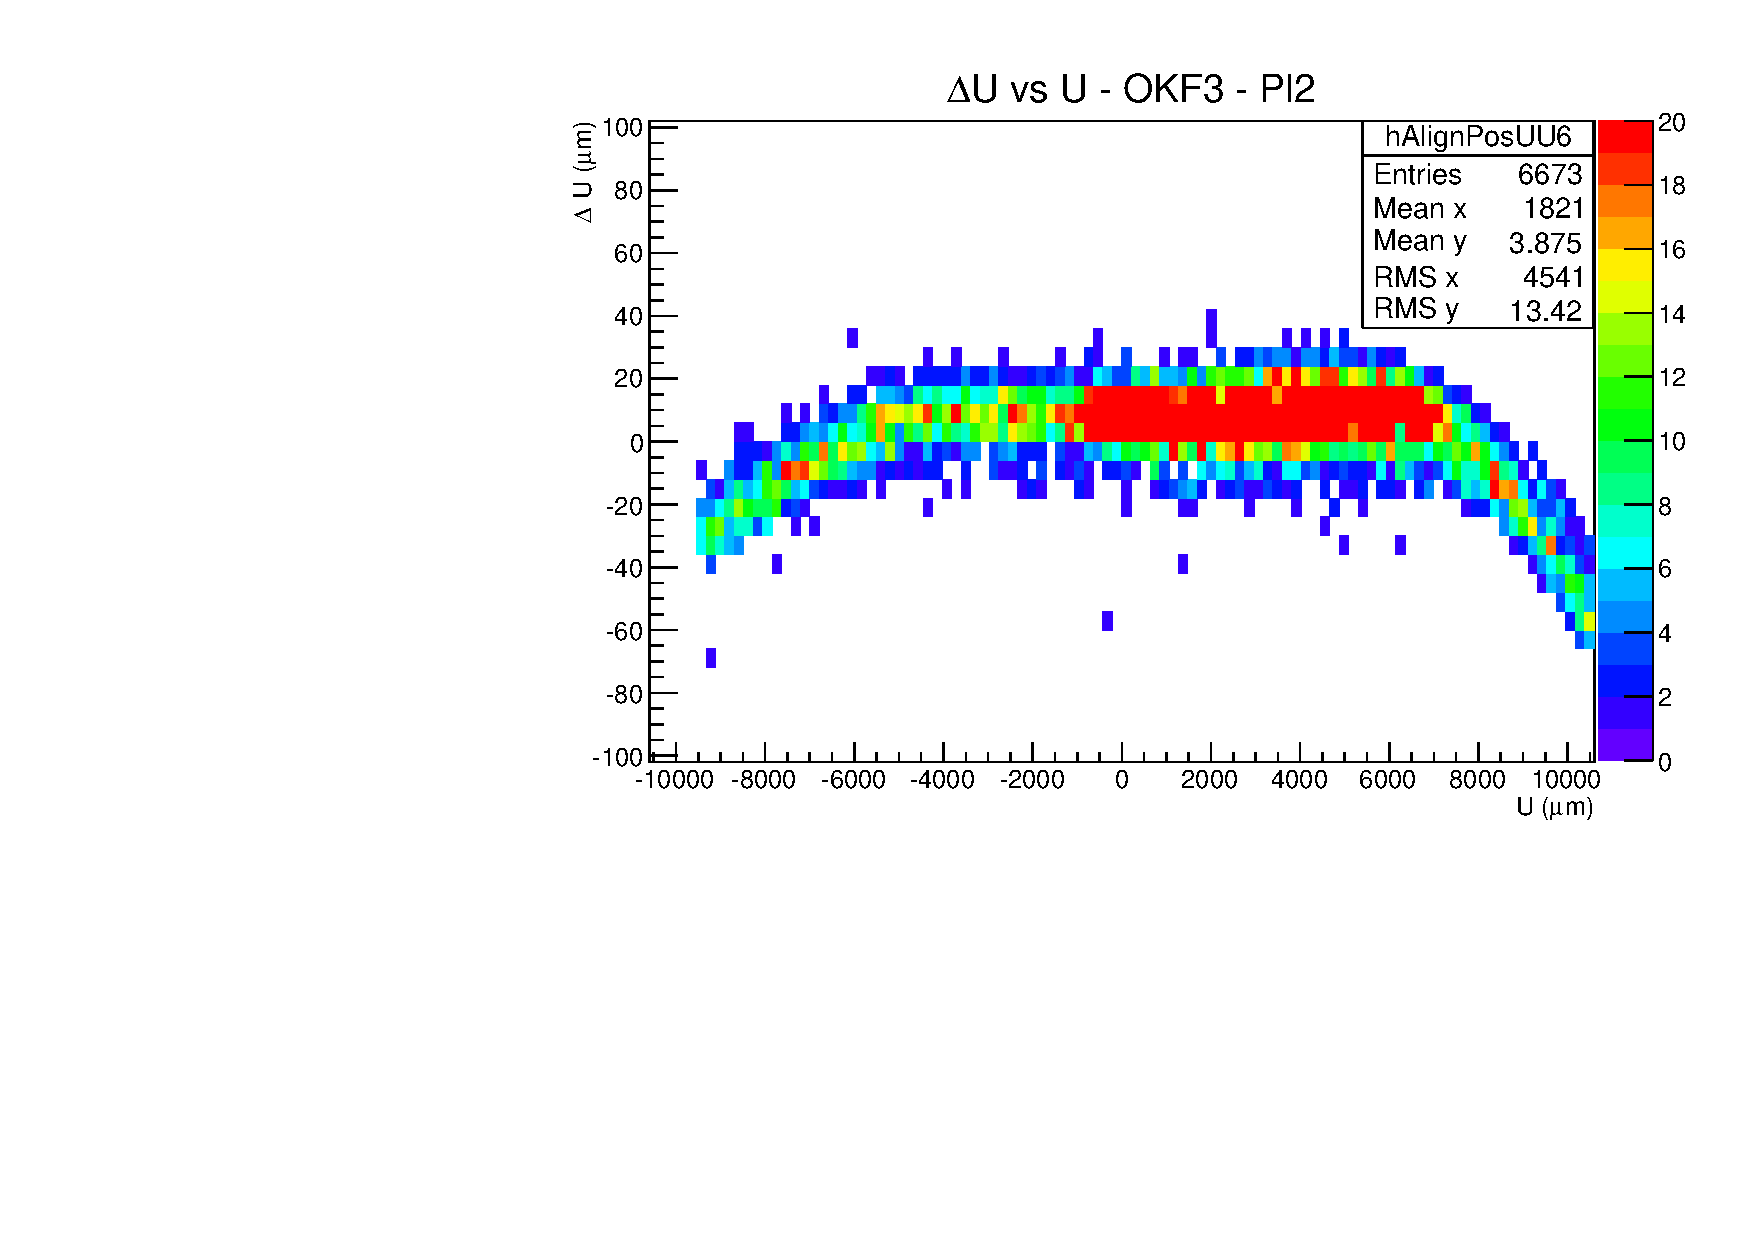
\includegraphics[scale=0.50]{./figures/PLUME_deformations/Du_v_U_Pl2_OKF3_Loic.pdf}
    \caption{Valeurs des r\'esidus en fonction de la position selon l'axe $U$ du capteur 2 de la face \textit{OKF3} inclin\'ee \`a 36 degr\'es.}
    \label{fig:Res_vs_U_banana}
   \end{center}
  \end{figure}
  
  Afin de visualiser les r\'esidus en fonction de la position sur le capteur, on peut par exemple r\'ealiser deux graphiques montrant les r\'esidus en fonction de la position de l'extrapolation de la trace sur l'axe horizontal $U$ et sur l'axe vertical $V$ du capteur consid\'er\'e. Lorsque l'\'echelle n'est pas inclin\'ee, on observe sur ces deux types de graphiques une bande horizontale et uniforme. La largeur de cette bande correspond \`a l'\'etendue de la distribution des r\'esidus. Cependant, lorsque l'\'echelle est inclin\'ee, les distributions des r\'esidus en fonction de la position l'axe $U$ des capteurs se transforment. On observe alors des motifs diff\'erents sur le graphique montrant les r\'esidus en fonction de la position selon l'axe $U$ du capteur consid\'er\'e. Les bandes homog\`enes obtenues \`a incidence normale sont d\'eform\'ees. On peut par exemple observer un motif incurv\'e vers le haut ou vers le bas. La figure \ref{fig:Res_vs_U_banana} illustre ce ph\'enom\`ene. On observe sur cette figure une forme incurv\'ee vers le bas. Les r\'esidus entre les postions $-10000 \, \mu m$ et $-6000 \, \mu m$ et $+7000 \, \mu m$ et $+11000 \, \mu m$ ont des valeurs jusqu'\`a quatre fois inf\'erieures par rapport \`a la bande centrale entre $-5000 \, \mu m$ et $+7000 \, \mu m$.
  
  \medskip
  
  On observe donc que les r\'esidus varient en fonction de la position $U$ sur le capteur. Cette variation des r\'esidus s'explique par la d\'eformation du capteur lors de la prise des donn\'ees. Voyons comment on peut mod\'eliser la variation des r\'esidus en fonction de la d\'eformation du capteur. La figure \ref{fig:DeformCMOS} sch\'ematise la d\'eformation d'un capteur pour des traces inclin\'ees selon l'axe vertical $V$ du capteur.

  \begin{figure}[!htb]
   \begin{center} 
    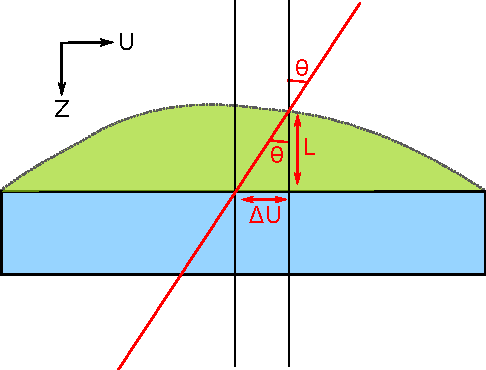
\includegraphics[scale=0.75]{./figures/deformations.pdf}
    \caption{Sch\'ema d'une d\'eformation d'un capteur CMOS. Le capteur sans d\'eformation est indiqu\'e en bleu. La surface du capteur d\'eform\'e suit l'extr\'emité sup\'erieure du volume vert.}
    \label{fig:DeformCMOS}
   \end{center}
  \end{figure}
  
  \medskip
  
  On peut alors exprimer la variation $dU$ d'un r\'esidu selon la direction $U$ du capteur en fonction du d\'ecalage $L$ selon l'axe $Oz$ du capteur et inversement.
   
  \begin{equation}
   dU = L \tan(\theta) \quad\quad L = \cfrac{dU}{\tan(\theta)}
  \label{eq:residusDeform}
  \end{equation}

  Le r\'esidu selon la direction $U$ calcul\'e pour chaque trace s'\'ecrit alors de la fa\c{c}on suivante :
  
  \begin{equation}
   \Delta U_{Deform} = \Delta U_{Non Deform} + dU
  \end{equation}
  
  On notera que comme les traces ne sont inclin\'ees que selon l'axe vertical $V$ du capteur, on n'observe une augmentation de la valeur des r\'esidus que selon l'axe horizontal $U$ du capteur. Les r\'esidus selon l'axe $V$ sont inchang\'es. Si les traces \'etaient inclin\'ees selon l'axe $U$ du capteur on aurait mesur\'e une augmentation de l'amplitude des r\'esidus uniquement selon l'axe vertical $V$ du capteur. 

  \begin{figure}[!htb]
   \begin{center} 
    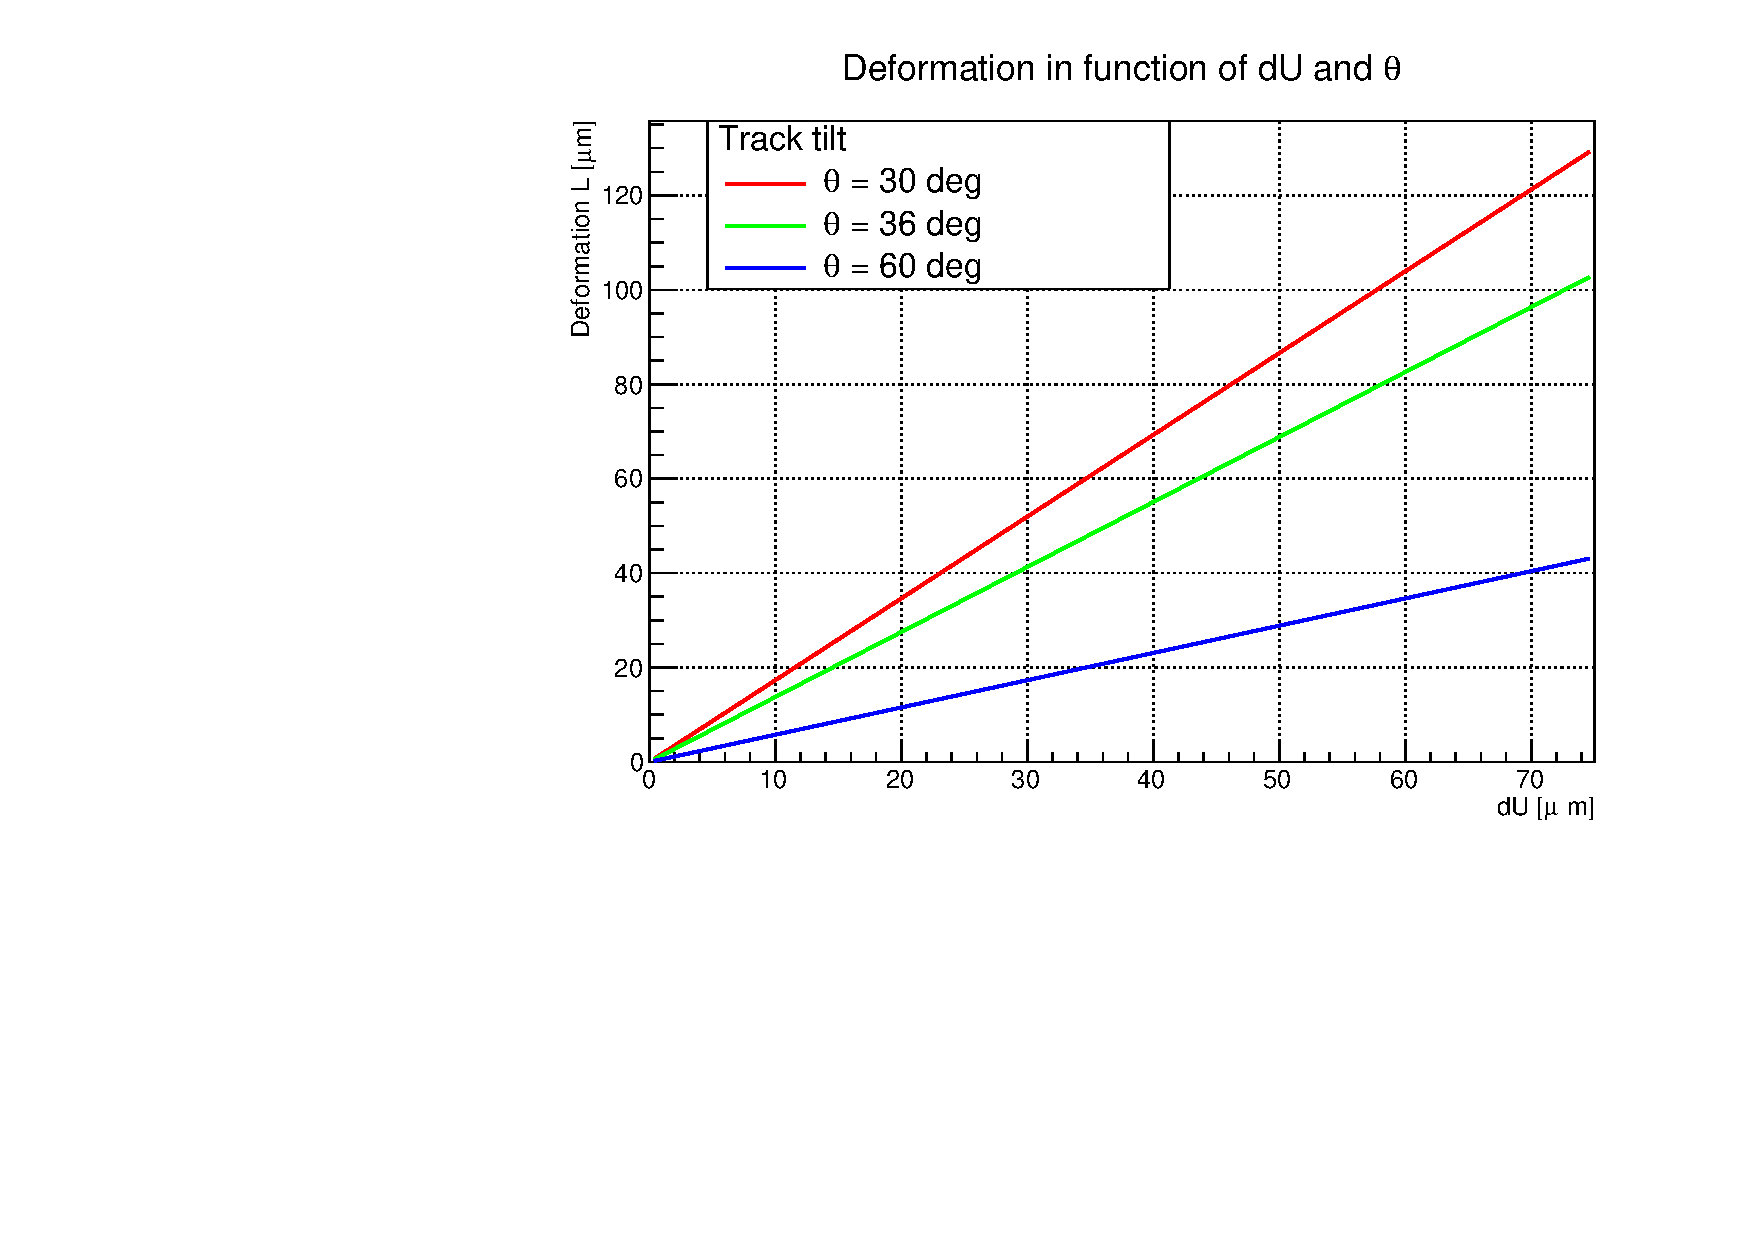
\includegraphics[scale=0.50]{./figures/PLUME_deformations/Deformations_theta.pdf}
    \caption{D\'eformation $L$ du capteur selon l'axe $Oz$ en fonction de l'augmentation du r\'esidu $dU$ et de l'angle d'incidence $\theta$ de la trace.}
    \label{fig:DeformationsTheta}
   \end{center}
  \end{figure}
  
  \medskip
  
  \`A partir de la relation \ref{eq:residusDeform}, on constate que plus la trace est inclin\'ee, plus l'augmentation des r\'esidus en fonction de la position $U$ sur le capteur est importante. On peut de plus remonter \`a la d\'eformation moyenne $L$ en fonction de la coordonn\'ee $U$ du capteur. La figure \ref{fig:DeformationsTheta} indique la d\'eformation $L$ du capteur selon l'axe $Oz$ en fonction de l'augmentation de l'amplitude du r\'esidu $dU$ et de l'angle d'incidence $\theta$ de la trace.
  
  \medskip
  
  Ainsi, lorsque qu'on se r\'ef\`ere \`a la figure \ref{fig:Res_vs_U_banana} on observe une augmentation de l'amplitude des r\'esidus maximale d'environ $dU_{max} = 50 \, \mu m$ en $U=10000 \, \mu m$. L'angle d'incidence des traces \'etant de 36 degr\'es, on remonte \`a un d\'ecalage maximal selon l'axe $Oz$ d'environ $L_{max} = 70 \, \mu m$. On peut supposer que ce d\'ecalage est provoqu\'e par une \'epaisseur de colle non uniforme qui incurverait le capteur \`a ces extr\'emit\'es.
  
  \medskip
  
  Pour conclure, les d\'eformations du capteur peuvent \^etre analys\'ees gr\^ace \`a une m\'ethode bas\'ee sur les traces \`a incidence non normale. La d\'eformation de la distribution des r\'esidus lorsque le capteur est d\'eform\'e induit un alignement d\'egrad\'e. Pour r\'esoudre cette difficult\'e, l'\'etude de l'alignement avec des capteurs d\'eform\'es et \`a incidence non normale, sur l'\'echelle \textit{PLUME}, est actuellement men\'ee par \textit{Benjamin Boitrelle}, doctorant \`a \textit{DESY} et travaillant en collaboration avec le groupe \textit{PICSEL}. L'alignement est alors r\'ealis\'e en ajoutant des degr\'es de libert\'e suppl\'ementaires repr\'esentant les d\'eformations du capteur.
  
%   \medskip
%   La figure repr\'esentant les distributions des r\'esidus selon l'axe horizontal $U$ et l'axe vertical $V$ des capteurs de l'\'echelle  arbore une allure diff\'erente lorsque l'\'echelle est inclin\'ee. Afin de visualiser les d\'eformations de la distribution des r\'esidus
%   
%   Les différents points ainsi repr\'esent\'es ne forment plus une bande et peuvent par exemple prendre la forme d'une banane. L'\'etude de ces d\'eformations est encore en cours. 
%   pour chaque coup en fonction des coordonn\'ees du coup dans le capteur
  
  \FloatBarrier
  
  \subsubsection{Mini-vecteurs}
  
  Nous allons \`a pr\'esent tester l'analyse de donn\'ees avec des mini-vecteurs. Les mini-vecteurs sont reconstruits de la mani\`ere suivante : apr\`es alignement, pour chaque trace reconstruite avec le t\'elescope, on recherche le coup le plus proche de la trace sur un des capteurs de la face OKF3. Puis, le coup le plus proche sur un des capteurs de la face OFK6 est à son tour s\'electionné. Le mini-vecteur est form\'e par ces deux coups. Le centre de chaque mini-vecteur, et les r\'esidus angulaires (angle du mini-vecteur moins angle de la trace) sont alors calcul\'es. La figure \ref{fig:resMiniVect} illustre les distributions des r\'esidus calcul\'ees sur chaque face de l'\'echelle, et avec le centre des mini-vecteurs. Ces distributions sont calcul\'ees selon l'axe vertical $V$ du capteur.
  
  \medskip
  
  \begin{figure}[!htb]
   \begin{center} 
    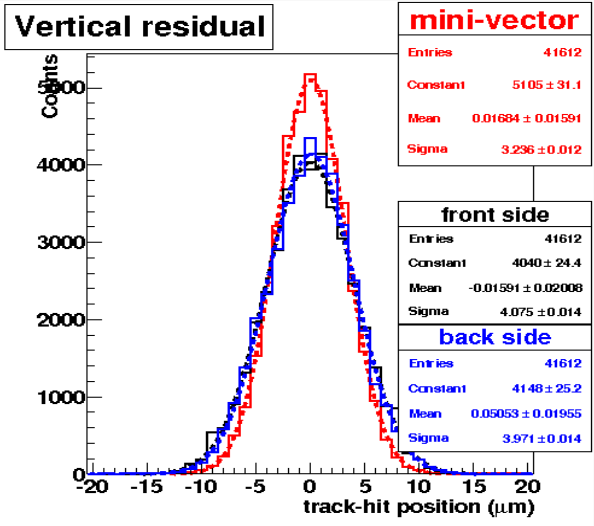
\includegraphics[scale=0.42]{./figures/PLUME_mini-vecteurs.png}
    \caption{Distribution des r\'esidus sur l'axe vertical (V) sur chaque face de l'\'echelle PLUME, (OKF3 en noir et OKF6 en bleu) et avec le centre des mini-vecteurs (en rouge)}
    \label{fig:resMiniVect}
   \end{center}
  \end{figure}
  
  Selon l'\'equation \ref{eq:propag_erreurs}, un facteur th\'eorique sur la r\'esolution spatiale valant $1/\sqrt{2}$ doit \^etre obtenu entre la r\'esolution sur une face et la r\'esolution sur le centre des mini-vecteurs. Pour v\'erifier ces assertions nous allons calculer les r\'esolutions pour chaque face de l'échelle, et pour le centre des mini-vecteurs. Le tableau \ref{tab:resol} r\'esume les valeurs trouv\'ees gr\^ace aux équations \ref{eq:propag_erreurs} et \ref{eq:resolution}.
  
  \begin{figure}[!htb]
   \begin{center} 
    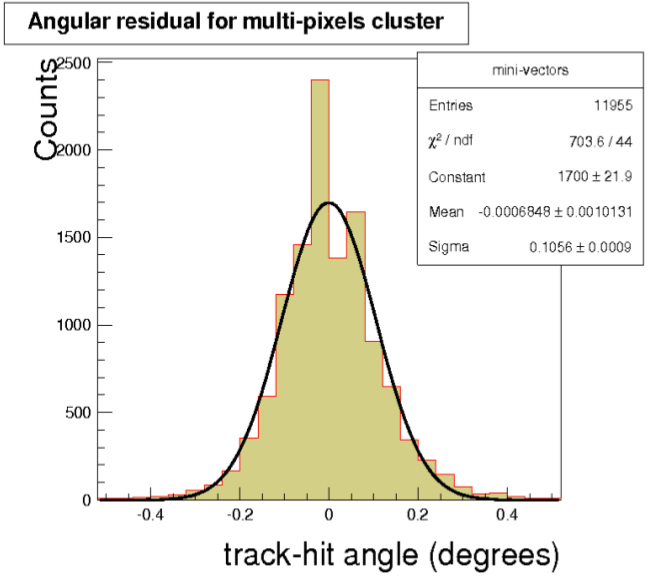
\includegraphics[scale=0.42]{./figures/PLUME_res_angulaire.png}
    \caption{Distribution des r\'esidus angulaires des mini-vecteurs}
    \label{fig:reso_ang}
   \end{center}
  \end{figure}
  
  \begin{table}[h]
  \begin{center}
  \small
  \begin{tabular}{|l|l|l|l|} \hline
                       & Largeur r\'esidus ($\mu m$) & R\'eso. tel. ($\mu m$) & R\'eso. DUT ($\mu m$) \\ \hline
  OKF3                 &   4.1                 &   1.8                       &        3.7       \\ \hline
  OKF6                 &   4.0                 &   1.8                       &        3.6       \\ \hline
  centre mini-vecteurs &   3.2                 &   1.8                       &        2.6       \\ \hline
  \end{tabular}
  \caption{Largeurs des distributions des r\'esidus et calculs des r\'esolutions en fonction de chaque couche de l'\'echelle PLUME et en fonction du centre des mini-vecteurs.}
  \label{tab:resol}
  \end{center}
  \end{table}
  
  Le rapport entre la r\'esolution au centre des mini-vecteurs et la r\'esolution sur la face OKF3 vaut $2.6/3.7 \approx 0.70 \approx 1/\sqrt{2} $ et le rapport entre la r\'esolution au centre des mini-vecteurs et la r\'esolution sur la face OKF6 vaut $2.6/3.6 \approx 0.72 \approx 1/\sqrt{2}$. L'am\'elioration attendue correspond bien aux rapports observ\'es.
  
  \medskip
  
  La figure \ref{fig:reso_ang} illustre la distribution des r\'esidus angulaires. L'\'ecart type de cette distribution vaut $0.11 \pm  0.01$ degr\'es. Nous exploiterons ce r\'esultat au chapitre \ref{chap:alignement} traitant de l'alignement d'\'echelles PLUME simul\'ees avec mini-vecteurs.

  \FloatBarrier
  
  \subsubsection{Conclusion}
  
  Afin de conclure l'\'etude de ce test en faisceau de l'\'echelle PLUME, nous allons en d\'egager les principaux enseignements. Premi\`erement, l'ensemble des capteurs de l'\'echelle r\'epondent de façon similaire. Les r\'esultats ainsi obtenus sont comparables avec le capteur de r\'ef\'erence MIMOSA 26 epi standard. Toutefois quelques \'ecarts sont visibles. Ils sont encore \`a l'\'etude. Du fait des faibles variations des param\`etres des capteurs mont\'es sur l'\'echelle observ\'ee, le refroidissement passif de l'\'echelle est valid\'e.
  
  \medskip
  
  Dans un second temps, l'\'etude des mini-vecteurs a permis de v\'erifier leurs comportements th\'eoriques. La r\'esolution attendue au milieu du mini-vecteur correspond bien \`a un facteur $1/\sqrt{2}$ de la r\'esolution sur les deux faces de l'\'echelle lui donnant naissance. De plus la r\'esolution angulaire des mini-vecteurs a \'et\'e \'etablie \`a $0.1$ degr\'e.

  \medskip
  
  A ce jour, l'\'etude de ce test en faisceau reste incompl\`ete. Les propri\'et\'es des capteurs de l'\'echelle inclin\'ee sont pr\'eliminaires et doivent \^etre confirm\'ees. De plus, des d\'eformations des capteurs mont\'es sur l'\'echelle ont \'et\'e mises en \'evidence. L'\'etude de ces d\'eformations est encore en cours lors de la r\'edaction de ce m\'emoire. 
  
  \medskip
  
  Une version am\'elior\'ee des échelles PLUME pr\'esent\'ees dans ce chapitre est en cours de conception. Les tests de ces nouvelles \'echelles sont pr\'evus pour mi-2015. Ces nouvelles \'echelles seront dot\'ees d'un budget de mati\`ere plus faible, de l'ordre de 0.30 $\% \, X0$ grâce \`a un support en carbure de silicium moins dense. Nous allons \`a pr\'esent traiter des tests en faisceau des super-plans SALAT.

  %   De plus la hauteur (direction $V$) de l'\'echelle a \'et\'e r\'eduite.
  
\section{SALAT}
  
  \subsection{Motivations}
  
  Comme nous l'avons vu au chapitre pr\'ec\'edent, le t\'elescope en faisceau de grande surface et de grande pr\'ecision, SALAT, sera un des constituants du t\'elescope en faisceau AIDA. Les prototypes des super-plans du t\'elescope SALAT, ont \'et\'e test\'es afin d'en mesurer leurs performances et de connaître leurs caract\'eristiques. Deux super-plans SALAT ont \'et\'e test\'es lors de la campagne de tests en faisceau de f\'evrier 2014 au \textit{Deutsch Synchrotron} (DESY) \`a Hambourg. Deux configurations ont \'et\'e mises en test. Une premi\`ere configuration constitu\'ee d'un t\'elescope de 4 capteurs MIMOSA-28 (alias ULTIMATE) et d'un super-plan SALAT et une seconde configuration compos\'ee de deux super-plans SALAT ont \'et\'e test\'ees.
  
  \medskip
  
  L'objectif principal de cette campagne de tests en faisceau \'etait de d\'emontrer le bon fonctionnement des super-plans SALAT. Pour cela l'homog\'en\'eit\'e de la r\'eponse de chaque capteur contenu dans un super-plan a \'et\'e \'etudi\'ee. Les param\`etres cl\'es de chacun de ces capteurs ont ainsi \'et\'e analys\'es en fonction du seuil de leurs discriminateurs. De plus, des \'etudes avec le super-plan inclin\'e ont \'et\'e r\'ealis\'ees. Elles permettront de conna\^itre, les variations des param\`etres cl\'es des capteurs composant le super-plan SALAT test\'e en fonction de son inclinaison. Et elles permettront aussi d'analyser les d\'eformations de la surface du super-plan \'etudi\'e.
  
  \subsection{Configuration exp\'erimentale : SALAT}

  Deux configurations ont \'et\'e mises en faisceau, l'une compos\'ee d'un t\'elescope \'equipé de quatre capteurs MIMOSA-28 et d'un super-plan SALAT et l'autre compos\'e de deux super-plans SALAT.
  
  \subsubsection{Super-plan SALAT}

   \begin{figure}[!htb]
    \begin{center} 
      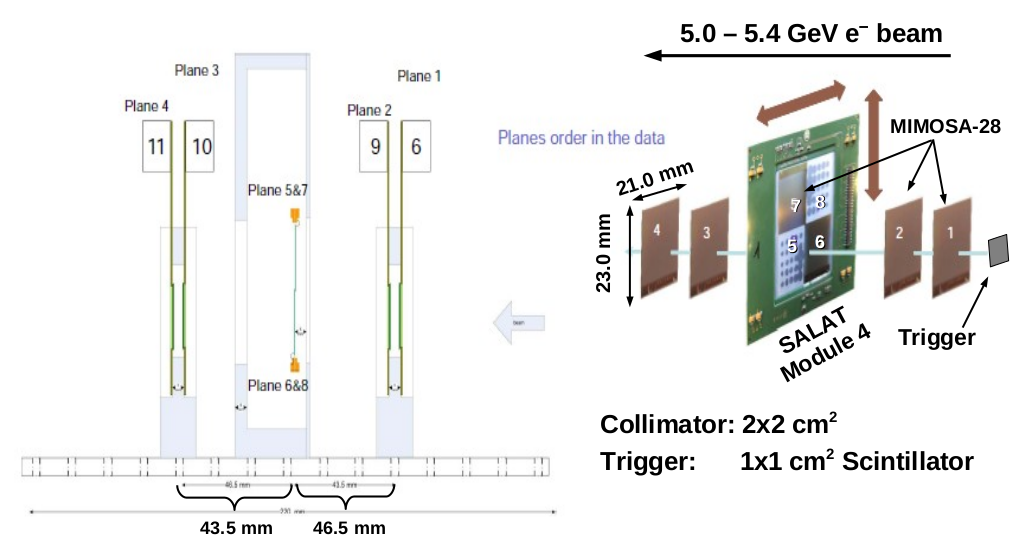
\includegraphics[scale=0.39]{./figures/SALAT_beam_test/SALAT_config.png}
      \caption{Configuration du t\'elescope pour l'\'etude d'un super-plan SALAT. Les distances inter-plans ainsi que la direction du faisceau sont indiqu\'ees.}
      \label{fig:config_SALAT_1}
    \end{center}
   \end{figure}
  
  Nous allons ici d\'ecrire la premi\`ere configuration test\'ee. Elle est compos\'ee d'un super-plan SALAT plac\'e \`a l'int\'erieur d'un télescope.
  
  \medskip

  Cette configuration est illustr\'ee en figure \ref{fig:config_SALAT_1}. Elle se compose d'un t\'elescope form\'e de quatre capteurs MIMOSA-28, r\'epartis en 2 bras. Le super-plan SALAT est lui dispos\'e entre ces deux bras. Son milieu d\'efinit la position de l'origine $O$ de l'axe Oz. Le premier bras  de t\'elescope croise le faisceau en premier et est plac\'e \`a -46.5 $mm$ du milieu du super-plan SALAT. Le capteur 1 croisant le faisceau en premier est ainsi dispos\'e \`a -47 $mm$ alors que le capteur 2, croisant le faisceau en second, est positionn\'e \`a -46 $mm$ sur l'axe Oz. Le second bras termine le t\'elescope et est plac\'e \`a +43.5 $mm$ du super-plan SALAT. Il est lui aussi compos\'e de 2 capteurs MIMOSA-28. Nous nommerons ces capteurs, capteur 3 et capteur 4. Le  capteurs 3 est positionn\'e \`a +43 $mm$ du centre du super-plan et le capteur 4 se situe \`a +44 $mm$. Chaque module est plac\'e perpendiculairement au faisceau. Les axes $Ox$ et $Oy$ sont respectivement parall\`eles aux  axes U et V des modules utilis\'es et leur origine est prise au point $O(0,0,0)$. Ainsi, l'origine du rep\`ere du t\'elescope correspond au point $O$. Un scintillateur de $1 \times 1$ $cm^2$ est plac\'e \`a l'avant du t\'elescope. Il est utilis\'e comme d\'eclencheur.
  
   \begin{figure}[!htb]
    \begin{center} 
      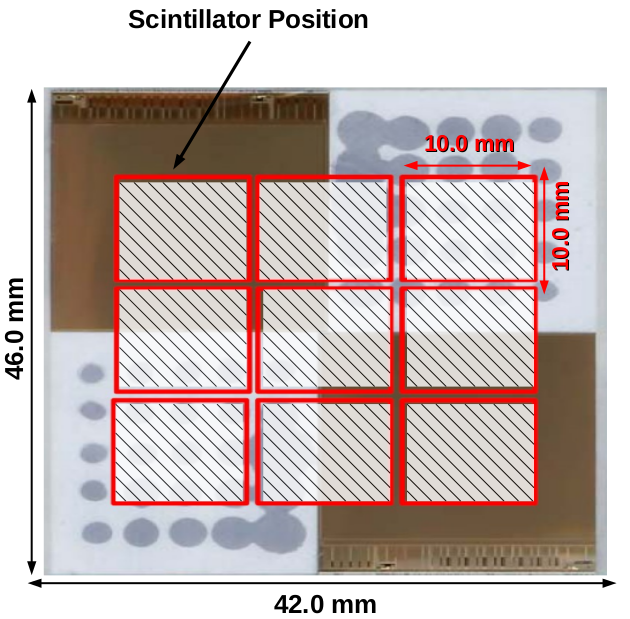
\includegraphics[scale=0.40]{./figures/SALAT_beam_test/beam_positions.png}
      \caption{Positions du faisceau utilis\'ees sur le super-plan SALAT lors des tests.}
      \label{fig:SALAT_zones}
    \end{center}
   \end{figure}

  Le faisceau de particules utilis\'e est un faisceau d'\'electrons dot\'es d'une impulsion comprise entre 5.0 et 5.4 $GeV$. Un collimateur de $2 \times 2$ $cm^2$ est utilis\'e. La r\'esolution du t\'elescope avec des particules d'impulsion infinie est estim\'ee \`a 1.8 $\mu m$. L'impulsion des \'electrons utilis\'es \'etant d'environ 5.0 $GeV$, la diffusion multiple n'est plus n\'egligeable. La r\'esolution du t\'elescope estim\'ee avec diffusion multiple est d'environ 2.2 $\mu m$ au niveau du super-plan SALAT.
  
  \medskip
  
  Les quatre capteurs constituant le super-plan utilis\'e sont num\'erot\'es de la façon suivante. En regardant le super-plan selon la direction du faisceau, le capteur 5 se trouve en bas \`a gauche sur la face arri\`ere du super-plan, le capteur 6 est localis\'e en bas \`a droite sur la face avant du super-plan, le capteur 7 se situe en haut \`a gauche sur la face avant du super-plan, et le capteur 8 est positionn\'e en haut \`a droite, sur la face arri\`ere du super-plan.
  
  \medskip
  
  Les capteurs formant le t\'elescope \'etant de surface inf\'erieure au super-plan SALAT, diff\'erentes positions du super-plan ont \'et\'e utilis\'ees afin de parcourir toute sa surface. La figure \ref{fig:SALAT_zones} illustre les 9 positions du faisceau utilis\'ees sur le super-plan SALAT. Pour chacune de ces r\'egions un balayage en seuil des discriminateurs des capteurs du super-plan SALAT a \'et\'e r\'ealis\'e. Les seuils utilis\'es sont de 5, 6, 8 et 10 fois le bruit moyen de chaque capteur. Toutefois, faute de temps, l'ensemble des seuils n'a pas \'et\'e test\'es. Seuls les seuils jug\'es les plus int\'eressants et repr\'esentatifs ont \'et\'e test\'es.
  
  \subsubsection{Proto-t\'elescope SALAT}
  
  Nous allons \`a pr\'esent d\'ecrire la seconde configuration test\'ee lors de cette campagne de tests en faisceau. Cette configuration est compos\'ee de deux super-plans SALAT formant un proto-t\'elescope. Rappelons que le t\'elescope SALAT sera compos\'e de 3 super-plans. Pour des raisons d'acquisition et de nombres de super-plans produits et fonctionnels seuls deux super-plans ont \'et\'e mis en test.

   \begin{figure}[!htb]
    \begin{center} 
      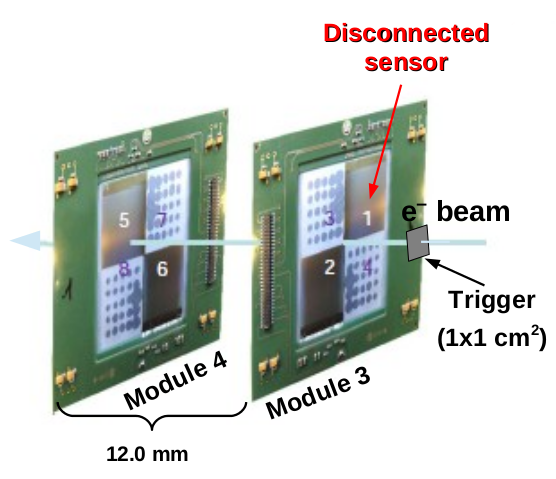
\includegraphics[scale=0.50]{./figures/SALAT_beam_test/config_proto_tel.png}
      \caption{Configuration du proto-t\'elescope. La distance inter-super-plan ainsi que la direction du faisceau et le d\'eclencheur sont indiqu\'es.}
      \label{fig:SALAT_proto_tel}
    \end{center}
   \end{figure}    
  
  \medskip
  
  La figure \ref{fig:SALAT_proto_tel} d\'ecrit la configuration du proto-t\'elescope mis en faisceau. Le t\'elescope est compos\'e de 2 super-plans SALAT, appel\'es module 3 et module 4, distants de 12.0 $mm$ selon l'axe Oz du faisceau. Le point $O$ de cet axe est d\'efini par l'endroit ou le faisceau traverse le premier super-plan (le module 3). Chaque module est plac\'e perpendiculairement au faisceau. Les axes $Ox$ et $Oy$ sont respectivement d\'efinis par les axes horizontaux U et verticaux V des modules utilis\'es et par le point $O(0,0,0)$. Un scintillateur utilis\'e comme d\'eclencheur, est plac\'e \`a l'avant du module 3. Le module 3 poss\`ede un de ses 4 capteurs endommag\'e. Bien que ce capteur soit en partie fonctionnel, celui-ci a \'et\'e d\'esactiv\'e lors des tests du proto-t\'elescope.
  
  \medskip
  
  Le faisceau de particules utilis\'e est un faisceau d'\'electrons d'une impulsion comprise entre 3 et 6 $GeV$. Les tests ont \'et\'e effectu\'es avec et sans le collimateur afin de maximiser (sans collimateur) la surface touch\'ee par le faisceau. Seulement deux super-plans sont utilis\'es pour le proto-t\'elescope ce qui r\'eduit les \'etudes possibles de trajectom\'etries. Nous nous int\'eresserons ainsi qu'aux seules associations entre les impacts sur le module 3 et les impacts sur le module 4 dans le but d'identifier des traces.
  
%   \subsection{DAQ}
  
  \subsection{R\'esultats}
  
  Les r\'esultats pr\'esent\'es ici ont principalement \'et\'e r\'ealis\'es par d'autres membres du groupe. On notera que pour l'acquisition, les quatre capteurs constituant chaque super-plan SALAT sont synchronis\'es.
  
  \subsubsection{Super-plan SALAT non inclin\'e}

  Nous commencerons l'\'enonc\'e des r\'esultats de cette campagne de tests en faisceau par les analyses du super-plan SALAT seul et ne poss\'edant aucune inclinaison. Nous d\'ecrirons l'alignement du t\'elescope utilis\'e et nous commenterons les r\'esultats obtenus pour les param\`etres cl\'es des capteurs composants le super-plan. Nous analyserons les donn\'ees obtenues puis nous examinerons l'homog\'en\'eit\'e de la r\'eponse de chacun des capteurs. Enfin, nous comparerons ces r\'esultats avec les donn\'ees extraites du test en faisceau du capteur de r\'ef\'erence MIMOSA-28 (epi standard) r\'ealis\'ees au SPS.
  
  \paragraph{Alignement du t\'elescope et du super-plan}
  
   \begin{figure}[!htb]
    \begin{center} 
      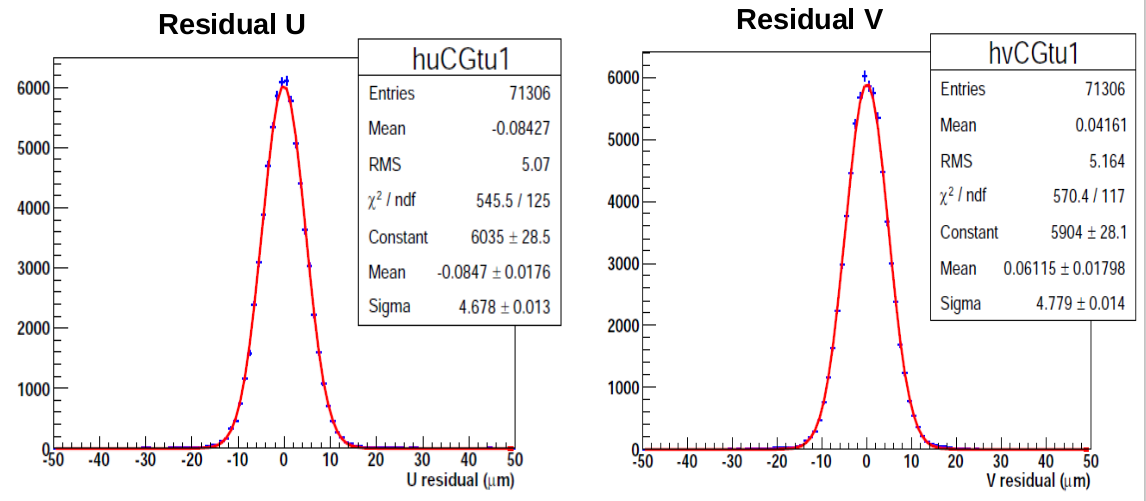
\includegraphics[scale=0.375]{./figures/SALAT_beam_test/residus_thr6xNoise_sensor5.png}
      \caption{R\'esidus sur le capteur 5, selon ses axes U et V, apr\`es alignement. Le capteur 5 est ici plac\'e dans le faisceau.}
      \label{fig:SALAT_residus_sensor_5}
    \end{center}
   \end{figure}
  
  Lors de l'\'etape d'alignement, le t\'elescope a tout d'abord \'et\'e align\'e sans prendre en compte le super-plan SALAT test\'e. Une fois le t\'elescope align\'e, chacun des quatre capteurs composant le super-plan SALAT test\'e \`a \'et\'e align\'e s\'epar\'ement. La figure \ref{fig:SALAT_residus_sensor_5} illustre la distribution des r\'esidus obtenue apr\`es alignement du capteur 5. L'alignement effectu\'e ici est r\'ealis\'e en supposant des traces rectilignes suivant la direction du faisceau. La diffusion multiple \'etant importante avec le faisceau de particules utilis\'e, les traces r\'eelles ne sont pas v\'eritablement rectilignes. Le $\chi^2$ des traces s'en voit ainsi affect\'e et l'alignement n'est plus aussi pr\'ecis qu'avec des traces v\'eritablement rectilignes (c'est-à-dire sans diffusion multiple). Les largeurs pour les distributions des r\'esidus sont compatibles avec la somme quadratiques de la r\'esolution du t\'elescope, corrig\'ee avec un terme de diffusion multiple estim\'ee, et de la r\'esolution spatiale du super-plan.
  
  \paragraph{Homog\'en\'eit\'e de la r\'eponse}
  
  \medskip
  
  Afin de tester l'homog\'en\'eit\'e de la r\'eponse des quatre capteurs composant le super-plan SALAT, chacun de ces capteurs a \'et\'e analys\'e s\'epar\'ement. L'efficacit\'e de d\'etection, le taux d'impacts fant\^omes, la multiplicit\'e des amas de pixels et la r\'esolution spatiale ont \'et\'e extraits sur chacun des 4 capteurs en fonction du seuil des discriminateurs appliqu\'e. Les r\'esultats de ces \'etudes sont pr\'esent\'es dans ce paragraphe.
  
  %   \begin{landscape}
   
     \begin{figure}[htb!]
     \begin{center}
        \subfigure[Efficacit\'es de d\'etection extraites en fonction de la zone test\'ee sur le super-plan SALAT (Module 4).]{
            \label{fig:SALAT_eff_pos}
            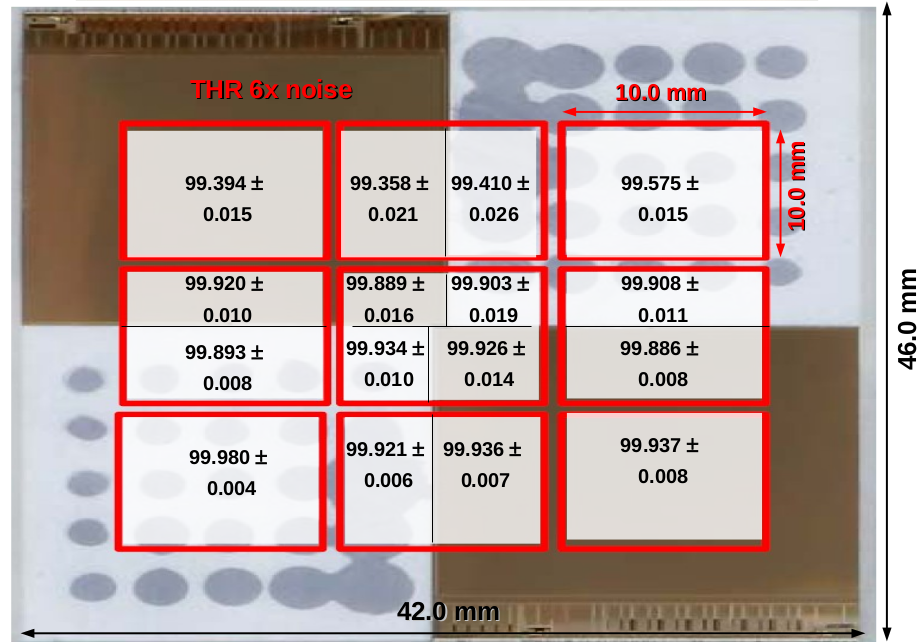
\includegraphics[width=0.68\textwidth]{./figures/SALAT_beam_test/effi_vs_position_thr6xnoise.png}
        }
        \subfigure[Largeurs des r\'esidus obtenues sur le super-plan SALAT (module 4) en fonction de la zone test\'ee.]{
           \label{fig:SALAT_res_6x_noise}
           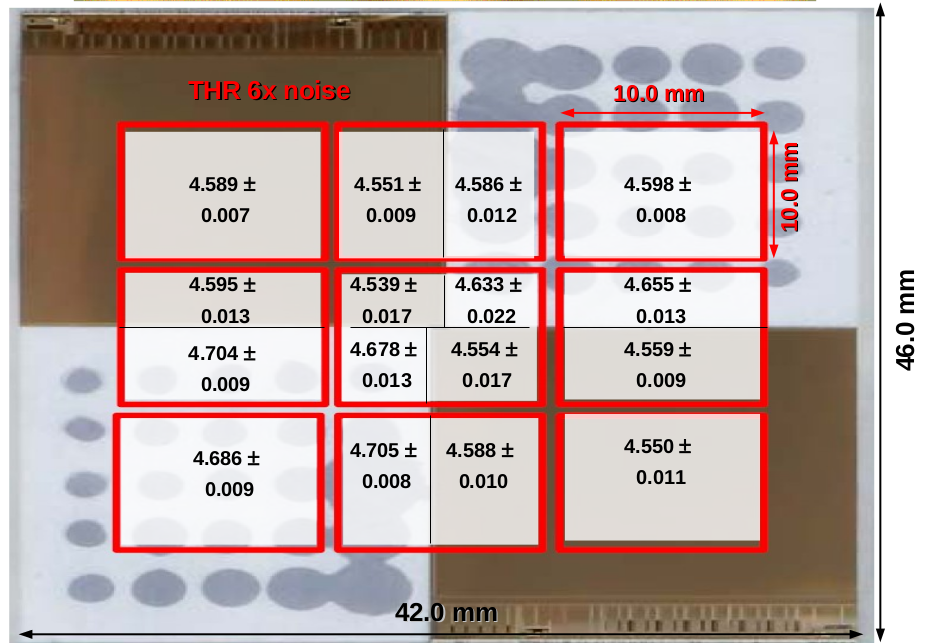
\includegraphics[width=0.68\textwidth]{./figures/SALAT_beam_test/Res_thr_6x_noise_position.png}
        }
     \end{center}
     \caption{Efficacit\'es de d\'etection et largeurs des distributions des r\'esidus en fonction de la zone du super-plan \'etudi\'ee. (Module 4)}
     \label{fig:zonesSALAT}
     \end{figure}
   
%   \end{landscape}
  
  \medskip

  La figure \ref{fig:SALAT_eff_pos} repr\'esente l'efficacit\'e de d\'etection obtenue en fonction des zones \'etudi\'ees sur le super-plan SALAT. Les efficacit\'es affich\'ees sur cette figure ont \'et\'e extraites \`a partir d'un seuil fix\'e \`a six fois le bruit moyen de chacun des capteurs. Globalement, la valeur de l'efficacit\'e sur l'ensemble du capteur est homog\`ene et vaut environ 99.9 $\%$. Toutefois, certaines zone du super-plan, ont une efficacit\'e inf\'erieure. Il s'agit des trois zones en haut du capteur (voir figure \ref{fig:SALAT_eff_pos}). Pour ces trois zones les efficacit\'es valent en lisant de gauche \`a droite la figure : 99.4, 99.4 et 99.6 $\%$. Ceci pourrait \^etre expliqu\'e par une erreur dans la valeur du seuil appliqu\'e aux discriminateurs de chaque capteur.
   
   \medskip
   
   La figure \ref{fig:SALAT_res_6x_noise} illustre la largeur de la distribution des r\'esidus obtenue sur chacune des zones indiqu\'ees. Le seuil des discriminateurs est r\'egl\'e \`a six fois le bruit moyen du capteur consid\'er\'e. Les valeurs obtenues pour les largeurs des distributions des r\'esidus sont similaires et appartiennent \`a un intervalle de 4.5 \`a 4.7 $\mu m$.
   
%    
%   \begin{figure}[!htb]
%     \begin{center} 
%       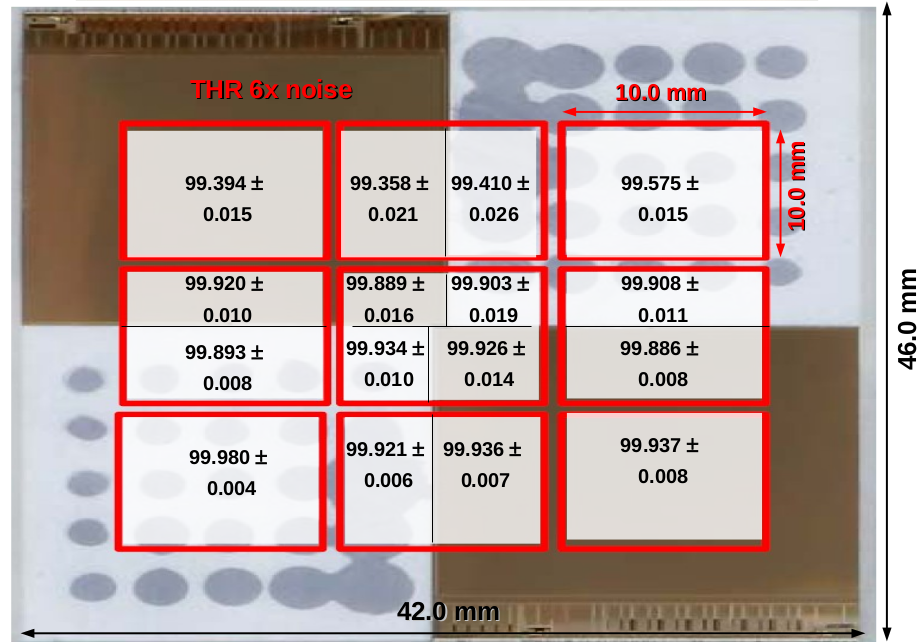
\includegraphics[scale=0.38]{./figures/SALAT_beam_test/effi_vs_position_thr6xnoise.png}
%       \caption{Efficacit\'es de d\'etection extraites en fonction de la zone test\'ee sur le super-plan SALAT (Module 3).}
%       \label{fig:SALAT_eff_pos}
%     \end{center}
%    \end{figure} 
%    
%    \begin{figure}[!htb]
%     \begin{center} 
%       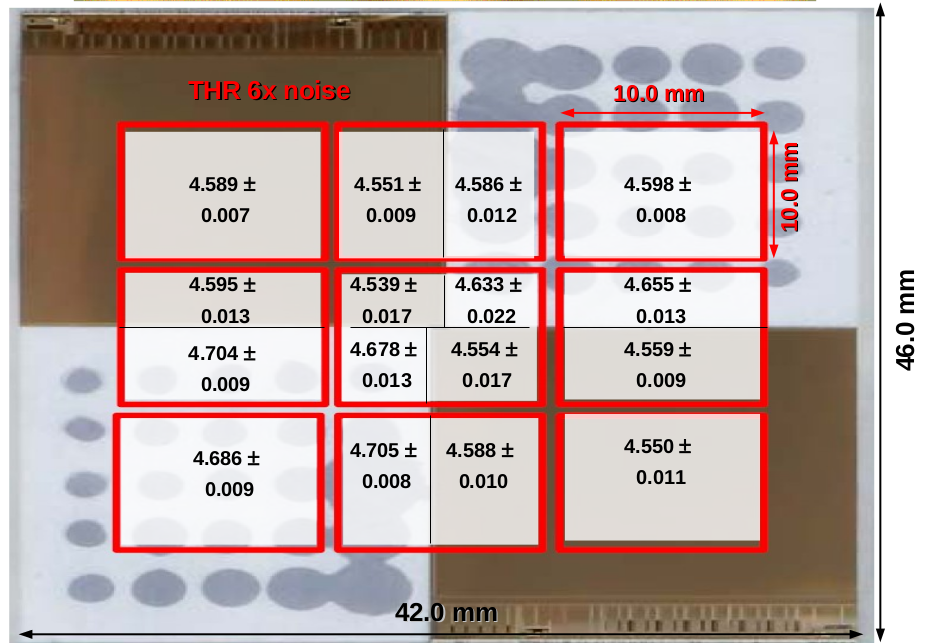
\includegraphics[scale=0.38]{./figures/SALAT_beam_test/Res_thr_6x_noise_position.png}
%       \caption{Largeurs des r\'esidus obtenues sur le super-plan SALAT (module 4) en fonction de la zone test\'ee.}
%       \label{fig:SALAT_res_6x_noise}
%     \end{center}
%    \end{figure}
  
  Les analyses ci-dessus ont \'et\'e r\'ealis\'ees avec tous les seuils et pour chaque param\`etre cl\'e des capteurs CMOS. Par la suite, les r\'esolutions spatiales de chaque capteur du super-plan seront extraites en fonction des largeurs des r\'esidus obtenues sur chaque capteur.

   \begin{landscape}
   
     \begin{figure}[htb!]
     \begin{center}
        \subfigure[Efficacit\'e de d\'etection pour chacun des quatre capteurs composant le super-plan SALAT test\'e (Module 4) en fonction du seuil des discriminateurs, compar\'ee au capteur de r\'ef\'erence MIMOSA-28.]{
            \label{fig:SALAT_eff}
            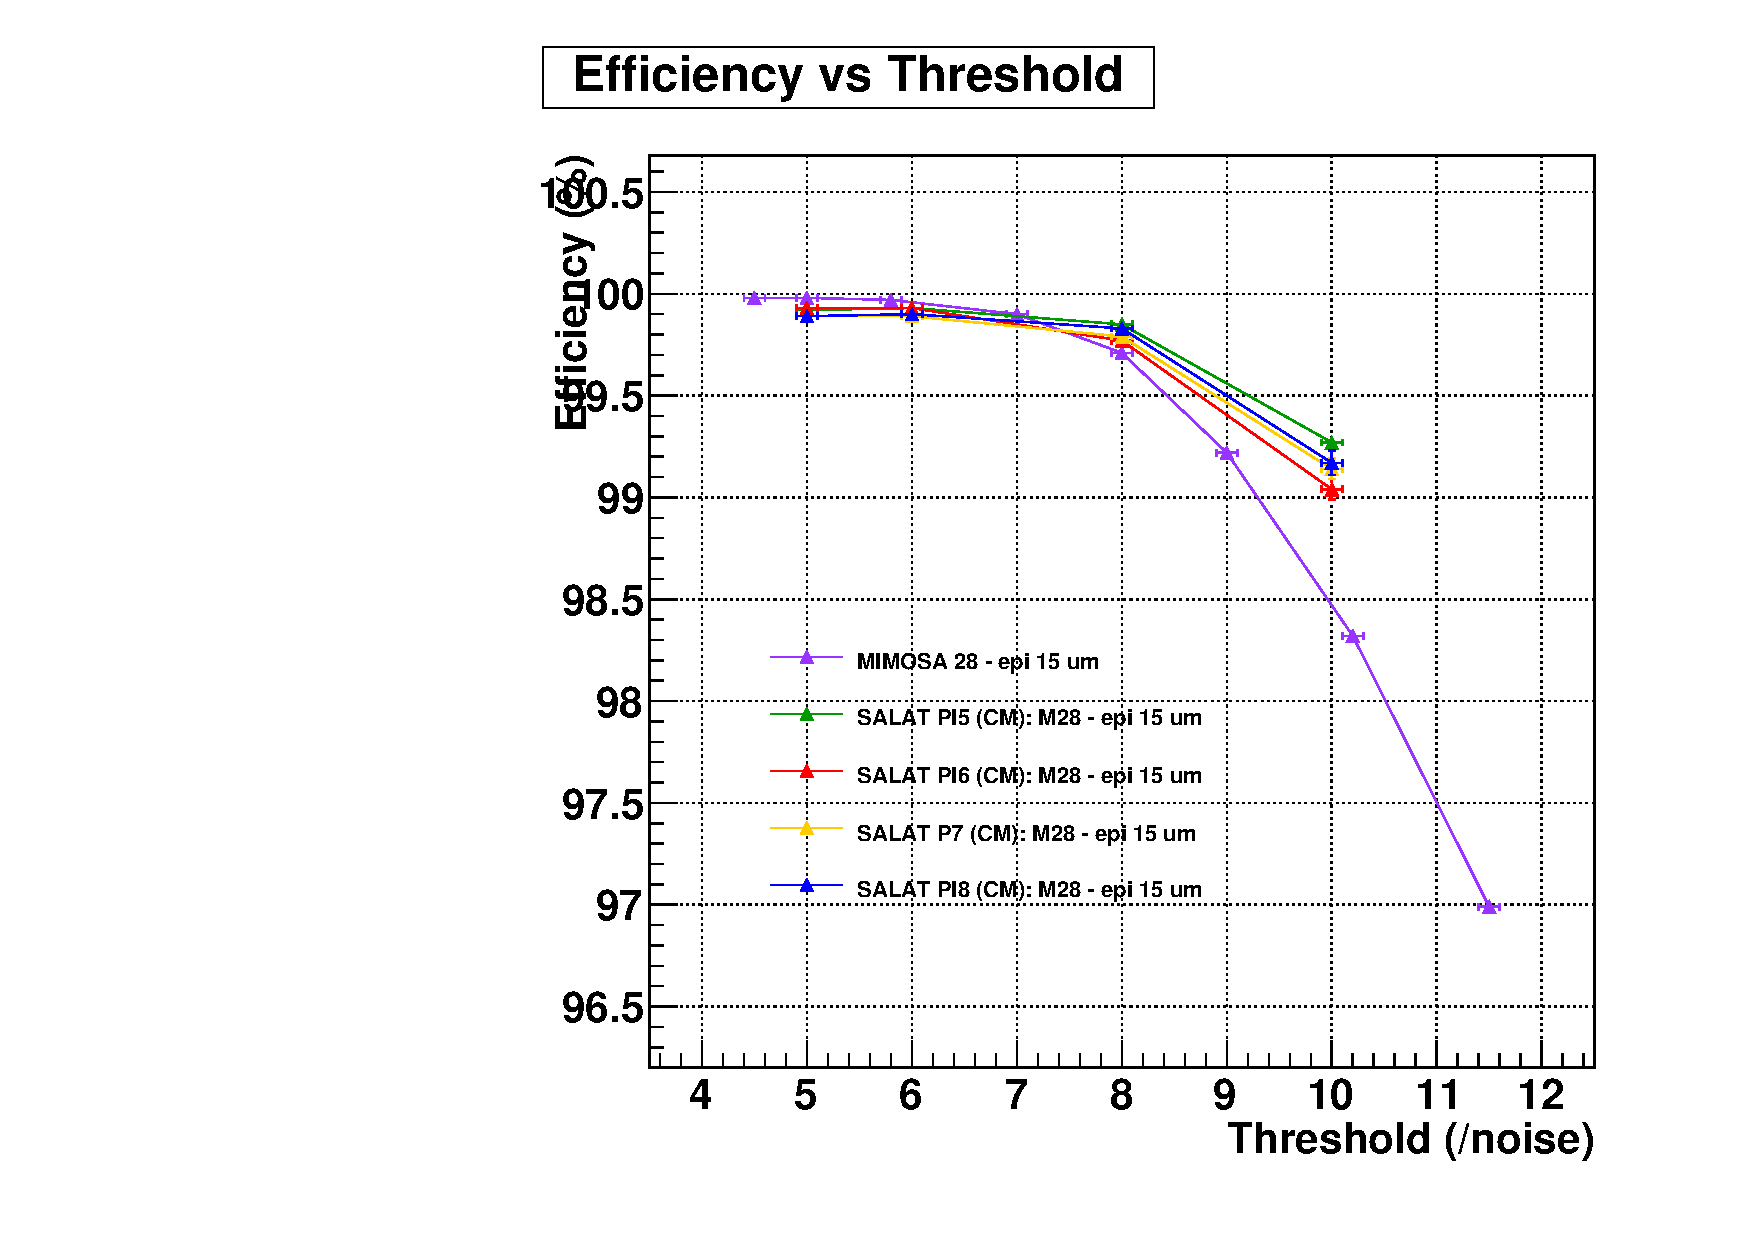
\includegraphics[width=0.67\textwidth]{./figures/SALAT_beam_test/Resultats/eff_vs_noise.pdf}
        }
        \subfigure[Taux d'impacts fant\^omes relev\'e pour chacun des quatre capteurs composant le super-plan SALAT test\'e (Module 4) en fonction du seuil des discriminateurs, compar\'ee au capteur de r\'ef\'erence MIMOSA-28.]{
           \label{fig:SALAT_fake}
           \includegraphics[width=0.67\textwidth]{./figures/SALAT_beam_test/Resultats/fake_hit_rate_vs_noise.pdf}
        }
     \end{center}
     \caption{Efficacit\'es et taux d'impacts fant\^omes pour les quatre capteurs composant le super-plan SALAT test\'e (module 4).}
     \label{fig:SALAT_EffFake}
     \end{figure}

   \end{landscape}

  \medskip
   
  La figure \ref{fig:SALAT_eff} repr\'esente l'efficacit\'e de d\'etection en fonction du seuil en multiple du bruit moyen pour chaque capteur composant le super-plan SALAT. Ces valeurs sont ensuite compar\'ees au capteur de r\'ef\'erence MIMOSA-28. Le module SALAT num\'ero 4 est ici utilis\'e. L'efficacit\'e obtenue pour chaque capteur est similaire \`a celle du capteur de r\'ef\'erence pour un seuil de discriminateurs compris entre 5 et 8 fois le bruit moyen. \`A plus haut seuil, l'efficacit\'e obtenue est sup\'erieure \`a celle de capteur de r\'ef\'erence. Ainsi, avec un seuil de dix fois le bruit moyen, l'efficacit\'e obtenue est d'environ 99.25 $\%$ alors que celle du capteur de r\'ef\'erence, r\'egl\'e au m\^eme seuil vaut 98.5 $\%$. On insistera sur le fait que le type de faisceau n'\'etait pas le m\^eme pour le capteur de r\'ef\'erence et pour le super-plan \'etudi\'e ici. Le capteur de r\'ef\'erence MIMOSA-28 a \'et\'e caract\'eris\'e avec un faisceau de pions charg\'es d'environ 100 $GeV/c$ au SPS alors que le super-plan SALAT test\'e ici a \'et\'e caract\'eris\'e avec un faisceau \'electrons d'environ 5 $GeV/c$ \`a DESY. Ainsi, une diff\'erence dans le d\'epôt de charges dans la couche \'epitaxi\'ee des capteurs peut \^etre observ\'ee. Or un plus fort d\'epôt de charges  induit un signal plus fort au niveau des pixels. Une augmentation du signal se traduit alors par une hausse de l'efficacit\'e et de la multiplicit\'e. C'est tr\`es certainement ce que nous observons ici. On notera que cet effet peut \^etre combin\'e avec de l\'eg\`eres variations induites par la calibration des capteurs. 
  
  \medskip
   
  La figure \ref{fig:SALAT_fake} indique le taux d'impacts fant\^omes en fonction du seuil en multiple du bruit moyen appliqu\'e aux discriminateurs des quatre capteurs du super-plan SALAT. Ces valeurs sont compar\'ees avec le capteur de r\'ef\'erence, MIMOSA-28. Les valeurs des taux d'impacts fant\^omes varient en fonction du capteur \'etudi\'e. Cependant, la dispersion du taux d'impacts fant\^omes en fonction du capteur \'etudi\'e ne d\'epasse pas un ordre de grandeur. De plus, la comparaison au capteur de r\'ef\'erence montre que le taux d'impacts fant\^omes des capteurs composant le super-plan SALAT, est sup\'erieur de maximum un ordre de grandeur. Ainsi au seuil de cinq fois la largeur moyenne du bruit, tous les capteurs poss\`edent un taux d'impacts fant\^omes en dessous de $3 \times 10^{-5}$ Ces valeurs \'elev\'ees du taux d'impacts fant\^omes sont tr\`es certainement le r\'esultat du non masquage des pixels chauds sur les quatre capteurs \'etudi\'es. En effet le taux d'impacts fant\^omes est domin\'e par un faible nombre de pixels ($<1\%$) appel\'es pixel chauds. Une analyse avec une coupure sur les pixels chauds devrait permettre de reproduire les bonnes valeurs pour le taux d'impacts fant\^omes. Faute de temps, cette \'etude n'a pas encore \'et\'e r\'ealis\'ee.
  
%    \begin{figure}[!htb]
%     \begin{center} 
%       \includegraphics[scale=0.60]{./figures/SALAT_beam_test/Resultats/eff_vs_noise.pdf}
%       \caption{Efficacit\'e de d\'etection pour chacun des quatre capteurs composant le super-plan SALAT test\'e (Module 4) en fonction du seuil des discriminateurs, compar\'ee au capteur de r\'ef\'erence MIMOSA-28.}
%       \label{fig:SALAT_eff}
%     \end{center}
%    \end{figure}
  
%    \begin{figure}[!htb]
%     \begin{center} 
%       \includegraphics[scale=0.60]{./figures/SALAT_beam_test/Resultats/fake_hit_rate_vs_noise.pdf}
%       \caption{Taux d'impacts fant\^omes relev\'e pour chacun des quatre capteurs composant le super-plan SALAT test\'e (Module 4) en fonction du seuil des discriminateurs, compar\'ee au capteur de r\'ef\'erence MIMOSA-28.}
%       \label{fig:SALAT_fake}
%     \end{center}
%    \end{figure}
   
   \begin{landscape}
   
     \begin{figure}[htb!]
     \begin{center}
        \subfigure[R\'esolution spatiale pour chacun des quatre capteurs composant le super-plan SALAT test\'e (Module 4) compar\'ee au capteur de r\'ef\'erence MIMOSA-28.]{
            \label{fig:SALAT_reso}
            \includegraphics[width=0.67\textwidth]{./figures/SALAT_beam_test/Resultats/res_vs_noise.pdf}
        }
        \subfigure[Multiplicit\'e des amas de pixels pour chacun des quatre capteurs composant le super-plan SALAT test\'e (Module 4) compar\'ee au capteur de r\'ef\'erence MIMOSA-28.]{
           \label{fig:SALAT_mult}
           \includegraphics[width=0.67\textwidth]{./figures/SALAT_beam_test/Resultats/mult_vs_noise.pdf}
        }
     \end{center}
     \caption{R\'esolutions spatiales et multiplicit\'e des amas de pixels pour les quatre capteurs composant le super-plan SALAT test\'e (module 4).}
     \label{fig:SALAT_ResMult}
     \end{figure}
   
   \end{landscape}
   
%    \begin{figure}[!htb]
%     \begin{center} 
%       \includegraphics[scale=0.60]{./figures/SALAT_beam_test/Resultats/res_vs_noise.pdf}
%       \caption{R\'esolution spatiale pour chacun des quatre capteurs composant le super-plan SALAT test\'e (Module 4) compar\'ee au capteur de r\'ef\'erence MIMOSA-28.}
%       \label{fig:SALAT_reso}
%     \end{center}
%    \end{figure}

%    \begin{figure}[!htb]
%     \begin{center} 
%       \includegraphics[scale=0.60]{./figures/SALAT_beam_test/Resultats/mult_vs_noise.pdf}
%       \caption{Multiplicit\'e des amas de pixels pour chacun des quatre capteurs composant le super-plan SALAT test\'e (Module 3
%       4) compar\'ee au capteur de r\'ef\'erence MIMOSA-28.}
%       \label{fig:SALAT_mult}
%     \end{center}
%    \end{figure}
  
  \medskip
   
  la figure \ref{fig:SALAT_reso} illustre la r\'esolution spatiale en fonction du seuil en multiple du bruit moyen appliqu\'e aux discriminateurs des quatre capteurs composant le super-plan SALAT. Les r\'esolutions obtenues sont compar\'ees \`a celles du capteur de r\'ef\'erence MIMOSA-28. Les r\'esolutions obtenues pour les quatre capteurs sont homog\`enes. Elles sont cependant plus hautes que celles du capteur de r\'ef\'erences, mais restent compatibles aux erreurs pr\`es. Ainsi au seuil de 8 fois le bruit moyen appliqu\'e aux discriminateurs, la r\'esolution spatiale vaut environ 3.7 $\mu m$. Cette valeur est \`a comparer au 3.5 $\mu m$ obtenue avec le m\^eme seuil, lors de l'analyse du capteur de r\'ef\'erence. On notera que la valeur de cette r\'esolution d\'epend de la valeur de la r\'esolution du t\'elescope \`a l'endroit de la mesure (voir \'equation \ref{eq:resolution}). A cause de la diffusion multiple lors des tests \`a DESY, cette valeur n'est pas connue avec pr\'ecision. On peut donc supposer que l'\'el\'evation de la r\'esolution des capteurs du super-plan SALAT, compar\'ee \`a celle du capteur de r\'ef\'erence est le r\'esultat d'une sous-estimation de la r\'esolution du t\'elescope (diffusion multiple sous-estim\'ee).
  
   \medskip
   
   La figure \ref{fig:SALAT_mult} donne les multiplicit\'es des amas de pixels en fonction du seuil en multiple du bruit moyen appliqu\'e aux discriminateurs de chacun des quatre capteurs du super-plan SALAT. Ces multiplicit\'es sont compar\'ees \`a celles du capteurs de r\'ef\'erence MIMOSA-28. Les multiplicit\'es obtenues pour chacun des quatre capteurs en fonction du seuil sont similaires. La multiplicit\'e moyenne varie ainsi d'environ 4.75 pixels par amas au seuil de 5 fois le bruit moyen, \`a 2.5 pixels par amas pour un seuil de 10 fois le bruit moyen. Ces valeurs sont plus \'elev\'ees de respectivement 1.25 et 0.3 pixels par amas pour les seuils de 5 et 10 fois le bruit moyen compar\'e au capteur de r\'ef\'erence. Cela correspond \`a une augmentation d'environ respectivement 35 $\%$ et 15 $\%$. Comme nous l'avons expliqu\'e pour l'efficacit\'e, une diff\'erence dans le d\'epôt de charge entre des pions d'environ 100 $GeV/c$ et des \'electrons de 5 $GeV/c$ pourrait expliquer ces diff\'erences. De plus, une anomalie dans la mise en amas des pixels touch\'es a r\'ecemment \'et\'e d\'ecouverte. Cette anomalie touche essentiellement les amas de haute multiplicit\'e. Une nouvelle m\'ethode de mise en amas a alors \'et\'e cr\'eée. Cette nouvelle m\'ethode sera utilis\'ee prochainement sur les donn\'ees de ce test en faisceau afin de v\'erifier si les multiplicit\'es extraites lors de cette campagne de test seront plus faibles \`a bas seuil.
   
   \FloatBarrier
   
  \paragraph{Super-plan SALAT inclin\'e}
  
  Afin, de d\'eterminer les propri\'et\'es du super-plan SALAT inclin\'e, celui-ci a \'et\'e test\'e avec une rotation selon son axe vertical V \`a partir d'un point sur l'axe horizontal U correspondant au milieu du super-plan. Des angles de 20 et 40 degr\'es ont \'et\'e utilis\'es. Une telle configuration permet de tester la variation des param\`etres cl\'es des capteurs composant le super-plan en fonction de l'angle utilis\'e mais aussi d'estimer les d\'eformations du super-plan. Ces deux \'etudes sont \`a l'heure de l'\'ecriture de cette th\`ese toujours en cours.
  
  \subsubsection{Proto-t\'elescope SALAT}
  
  Nous allons \`a pr\'esent \'etudier les r\'esultats de la seconde partie de la campagne de tests en faisceau des super-plans SALAT, o\`u deux super-plans SALAT forment un proto-t\'elescope. Nous d\'ecrierons dans un premier temps l'alignement du proto-t\'elescope puis nous r\'ealiserons une \'etude sur la trajectom\'etrie, bas\'ee sur les deux super-plans.
  
  \paragraph{Alignement du proto-t\'elescope}
  
  Pour aligner le proto-t\'elescope, le module 4 (contenant le super-plan SALAT test\'e seul) est utilis\'e comme plan de r\'ef\'erence. Les positions de chacun des quatre capteurs le composant sont fix\'ees en reprenant l'alignement effectu\'e lors de l'\'etude pr\'ec\'edente. Chacun des trois capteurs actifs (1 capteur d\'esactiv\'e) du super-plan contenu dans le module 3 sont alors align\'es individuellement. Pour chaque impact d\'etect\'e sur les capteurs du module 4, une trace est cr\'e\'ee. Pour cet alignement, on suppose les traces rectilignes et perpendiculaires aux capteurs du module 4. On utilise une m\'ethode bas\'ee sur la minimisation de l'ensemble des $\chi^2$ reconstruits sur chacun des 3 capteurs  du module 3 (pour plus de d\'etail sur l'alignement, voir la sous-section \ref{sect:alignement}). Les r\'esidus obtenus sur l'un des capteurs du module 3 sont visibles en figure \ref{fig:Align_proto_tel}
  
   \begin{figure}[!htb]
    \begin{center} 
      \includegraphics[scale=0.50]{./figures/SALAT_beam_test/residus_super-plan-3_proto_tel.png}
      \caption{R\'esidus sur un des capteurs du super-plan contenu dans le module num\'ero 3.}
      \label{fig:Align_proto_tel}
    \end{center}
   \end{figure}
  
  \paragraph{R\'esultats}

  Les \'etudes men\'ees avec le proto-t\'elescope SALAT mis en faisceau concernent la trajectom\'etrie. Comme le t\'elescope SALAT \'etudi\'e est constitu\'e de seulement 2 super-plans, les études possibles concernant la trajectom\'etrie sont restreintes. Aussi, on se limitera \`a l'\'etude des associations entre l'extrapolation des traces, cr\'e\'ees \`a partir du premier super-plan (module 4) sur le second super-plan (module 3), avec les impacts d\'etect\'es sur le second super-plan.
  
  \medskip

  Pour cette \'etude, les traces sont reconstruites \`a partir d'un impact initial sur l'un des quatre capteurs du module 4. \`A chaque impact sur les capteurs du module 3 est associ\'e une trace. La position de l'impact correspond au centre de gravit\'e de l'amas consid\'er\'e. La pente et la direction de chacune des traces sont d\'efinies comme parall\`eles au faisceau et de m\^eme direction que celui-ci. (Les traces ont donc un vecteur directeur valant (0,0,1) dans le rep\`ere du t\'elescope).
  
  \medskip

  Pour rappel, la trajectom\'etrie utilis\'ee dans le logiciel d'analyse TAF, associe l'impact le plus proche de l'extrapolation de la trace sur le capteur consid\'er\'e (dans une certaine fen\^etre de recherche). Puis la trace est ajust\'ee avec le nouvel impact. Dans notre cas la trace est d\'efinie \`a l'aide d'un seul impact et d'une direction. L'\'etude consiste alors \`a \'etudier les associations entre l'intersection des traces avec les capteurs du module et les impacts  r\'eels sur les capteurs du module 3.
  
   \begin{figure}[!htb]
    \begin{center} 
      \includegraphics[scale=0.37]{./figures/SALAT_beam_test/correl_zone_trig_no_hot_px.png}
      \caption{Affichage de 50 \'ev\'enements comportant en moyenne 12 traces. Sont repr\'esentés en bleu les intersections des traces avec les capteurs du module 3; et en rouge les impacts sur les capteurs du module 3. La zone couverte par le scintillateur est indiqu\'ee par un rectangle vert. Les pixels chauds ont \'et\'e retir\'es.}
      \label{fig:associations_super_plan_trigger}
    \end{center}
   \end{figure}
   
   \begin{figure}[!htb]
    \begin{center} 
      \includegraphics[scale=0.37]{./figures/SALAT_beam_test/hits_correlations_super_plan.png}
      \caption{Affichage de 50 \'ev\'enements comportant en moyenne 12 traces. Sont repr\'esentés en bleu les intersections des traces avec les capteurs du module 3; et en rouge les impacts sur les capteurs du module 3. La zone couverte par le scintillateur est indiqu\'e par un rectangle vert.}
      \label{fig:associations_super_plan}
    \end{center}
   \end{figure} 
  
  \medskip
  
  La figure \ref{fig:associations_super_plan} repr\'esente les intersections des traces issues des impacts sur les capteurs du module 4 et les impacts d\'etect\'es sur les capteurs du module 3. Sur cette figure, les pixels chauds ne sont pas \^otés. 

  \medskip
  
   La figure \ref{fig:associations_super_plan_trigger} est un agrandissement de la figure \ref{fig:associations_super_plan}. La zone d\'efinie par le scintillateur est alors affich\'ee. Sur cette figure, les pixels chauds ont \'et\'e retir\'es. On observe clairement une bonne association des impacts sur les capteurs du module 3 avec l'extrapolation des traces.
  
  \FloatBarrier
  
  \subsection{Conclusion}
  
  Pour conclure sur cette campagne de tests en faisceau, nous mettrons l'accent sur l'homog\'en\'eit\'e et le bon fonctionnement des super-plans SALAT. En effet, lors de ces tests des super-plans SALAT, nous avons observ\'e une r\'eponse similaire de chaque capteur compar\'e au capteur de r\'ef\'erence MIMOSA-28. Le type de refroidissement, par simple flux d'air, est de surcro\^it valid\'e. Ainsi, les super-plans SALAT sont prêts pour la production. Il pourront ainsi \^etre utilis\'es pour constituer un bras de t\'elescope de grande surface et de grande pr\'ecision. Enfin, des tests en faisceau du t\'elescope SALAT compos\'e de trois super-plans seront r\'ealis\'es fin novembre 2014.
  
\section{Conclusion des tests en faisceau de PLUME et SALAT}

 Dans ce chapitre nous avons \'enum\'er\'e les r\'esultats des campagnes de tests en faisceau des \'echelles PLUME et des super-plans SALAT. Nous en avons expos\'e les diff\'erentes caract\'eristiques. Les capteurs composant ces deux objets ont \'et\'e caract\'eris\'es et compar\'es entre eux. Les prototypes test\'es ont montr\'e une bonne homog\'en\'eit\'e de de leur r\'eponse et leur fonctionnement a \'et\'e valid\'e. De nouvelles \'echelles PLUME sont en d\'eveloppement et devraient être test\'ees mi-2015 et un bras de t\'elescope SALAT devrait bientôt voir le jour. Afin de pouvoir \'etudier les m\'ethodes de trajectom\'etrie possibles avec de tels objets, une simulation num\'erique des \'echelles PLUME et des super-plans SALAT a \'et\'e entreprise. La r\'ealisation et la description de cette simulation constituent le prochain chapitre.